\documentclass[11pt,a4paper]{article}
\usepackage[utf8]{inputenc}
\usepackage[spanish]{babel}
\usepackage{amsmath}
\usepackage{amsfonts}
\usepackage{amssymb}
\usepackage{makeidx}
\usepackage{graphicx}
\usepackage{multicol}
\usepackage{changepage}
\usepackage{float}
\usepackage{cite}
\usepackage{anyfontsize}
\usepackage{lmodern}
\usepackage{kpfonts}
\usepackage{fourier}
\usepackage[left=2cm,right=2cm,top=2cm,bottom=2cm]{geometry}
\author{Rodriguez Lopez Francisco Javier.\\Guzman Vazquez Jaime Alan Yamil.}
\title{Circuitos de Rectificacion no controlados}


\begin{document}
\begin{center}
\textbf{UNIVERSIDAD POLITECNICA DE LA ZONA METROPOLITANA DE GUADALAJARA}\\

\begin{figure}[hbtp]
\centering

\includegraphics[width=10cm]{Escritorio/Practica 1/Upzmg.png}
\caption{Institucion}
\end{figure}\\
\end{center}

Practica: Circuitos de Rectificacion no Controlados.\\
Nombre: Rodriguez Lopez Francisco Javier.\\
                  Guzman Vazquez Jaime Alan Yamil.\\
Fecha: 19 de septiembre del 2019.\\
Curso: Septiembre-Diciembre 2019c.\\
Docente: Moran Garabito Carlos Enrique.\\


\newpage
\section{Introduccion:}
En este reporte se abundara en todas las cuestiones que se refieren a la prac-
tica que se realizo en la semana anterior, la practica consistia en generar las
seales de diferentes partes en diferentes esquematicos , ejemplificando esto
tenemos la seal de un duplicador de tension que como lo dicta su nombre
duplica la tension de la salida de una seal, estos cinco circuitos fueron re-
alizados en el software de diseo de circuitos profesional OrCAD que es un
software de grado industrial diseado para generar cualquier tipo de simula-
cion por medio del simulador llamado PSPICE que te permite controlar y
manipular diferentes seales asi com ampliarlas o minimizarlas para conseguir
los graficos necesarios para la practica.\\
Los diodos conllevados, para hacer el paro de corriente en un cierto punto de cualquie sistema o circuito que este, este manejando, dando alternativas de generacion de transformacion de energia y como el mismo puede ser de mucha aplicacion en rangos de cualquier tipo. Comprobando su estabilidad de paro, y de fluidez a la hora de emplearse en sistemas mas complejos y de mayor alcance, ya sea este local, industrial, o como en este caso, por pura comprobacion puesta en simulaciones.\\
Asi pues explicaremos todo el contexto de estos circuitos y sus diferentes
aspectos asi como el uso que se les da en la industria, esto sera explicado en
el marco teorico en donde abundaremos en estas cuestiones, a continuacion
se explicara el desarrollo de la practica en donde se expliicaran los paso que
se siguieron en esta a continuacion y ya esxplicada la misma se procedera a
dar la conclusiones de cada uno de los colaboradores de forma independiente,
esta sera la manera que se realizara este documento.\\



\section{Objetivo:}
Ver el uso y la aplicacion de la Rectificacion en circuitos monofasico y trifasicos.


\section{Materiales:}
\begin{enumerate}
\item \textbf{Software OrCAD.}
\item \textbf{Computadora.}
\end{enumerate}



\section{Procedimiento:}
De aqui en adelante se estara redactando, cada diagrama esquematico simulado en esta practica, para tener la explicita idea de lo que se hizo en ello.\\
\begin{enumerate}
\item \textbf{Rectificador de media onda con carga inductiva:}
\begin{figure}[hbtp]
\centering
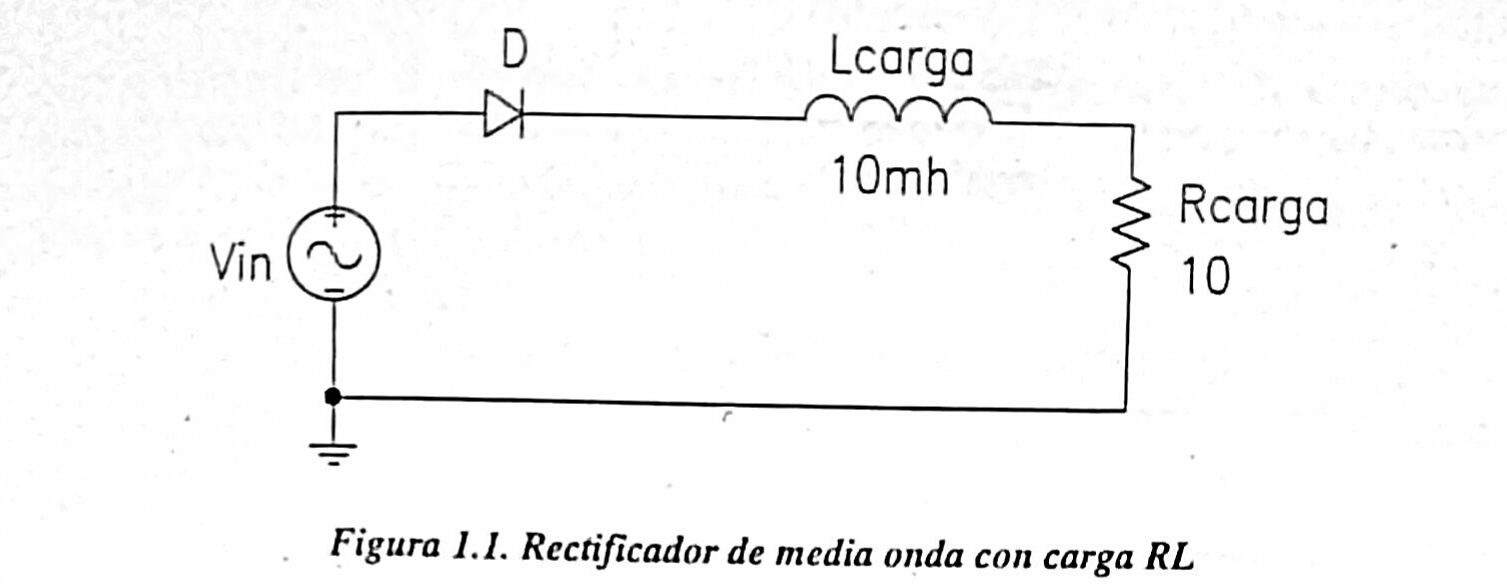
\includegraphics[width=7cm]{Escritorio/Practica 1/f.jpg}
\caption{Rectificador de media onda}
\end{figure}


En este diagrama lo que se trato, es ver de que forma y de que manera los componentes a tratar que sirven, el diodo rectificador y la bobina inductiva, cumplen su funcion. Por una parte el diodo, como ya sabemos hace el paro de corriente en la parte positiva de el inductor, lo que hace que la energia fluya en amplitud completa.\\
 Lo que hace que el inductor cumpla su funcion, cuando este recibe la corriente de la resistencia, genera un campo magnetico, lo que hace que alcance el rango de la onda, cumpliendo con la inductancia.
 
 \item \textbf{Rectificador Monofasico en Fuente:}
 \begin{figure}[hbtp]
 \centering
 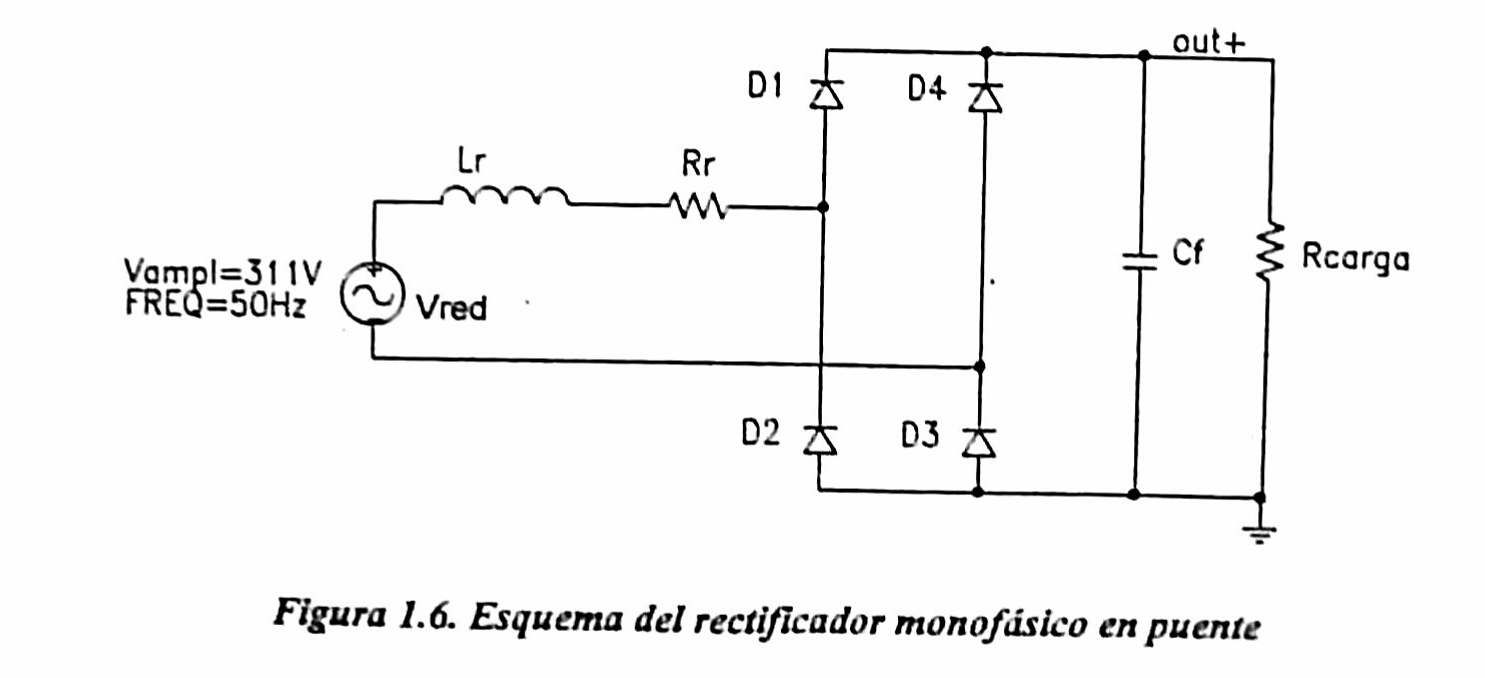
\includegraphics[width=7cm]{Escritorio/Practica 1/g.jpg}
 \caption{Rectificador monofasico en fuente}
 \end{figure}
 
 
 Para este diagrama, lo que se busco es ver nuevamente la rectificacion en marcha, y para hacerlo en una fase monofasica, lo que se puso en condicion al otro diagrama, es la vista y el uso del capacitor, como sabemos el capacitor cumple la funcion de un almacen de energia, lo que hace que las ondas generadas, por la simulacion, sean no totalmente senoidales, sino que en cada onda hay una distorsion, que se nota a la hora de colocar las puntas de prueba en voltaje, lo que pasa es que se aprecia la subida de voltaje en las ondas, y como estas se comportan.\\
 Este diagrama, no solo nos deja ver la influencia que tiene el capacitor en el diagrama, sino que tambien, se puede notar, como las puntas de prueba cuando estas son de voltaje, conectadas directamente a la fuente de poder(alterna), esta no pierde sus ondas senoidales, sino que siguen iguales, es decir, que si la prueba es conectarse a la fuente alterna, de forma directa, este no cambiara sus ondas, caso contrario que si lo conectaramos en otros lados, ya sea el inductor, el diodo, el capacitor, o la resistencia, en donde se puede apreciar desde la parte del puente de los cuatro diodos, como este va perdiendo energia, y recuperandola en partes.\\
 Formula utilizada:\\
 \emph{fourier}
 $$ i_{Lr}(t)= C_o + \sum_{n=1}{\infty} C_n sen(nw*t + o_$$

 
 \begin{figure}[hbtp]
 \centering
 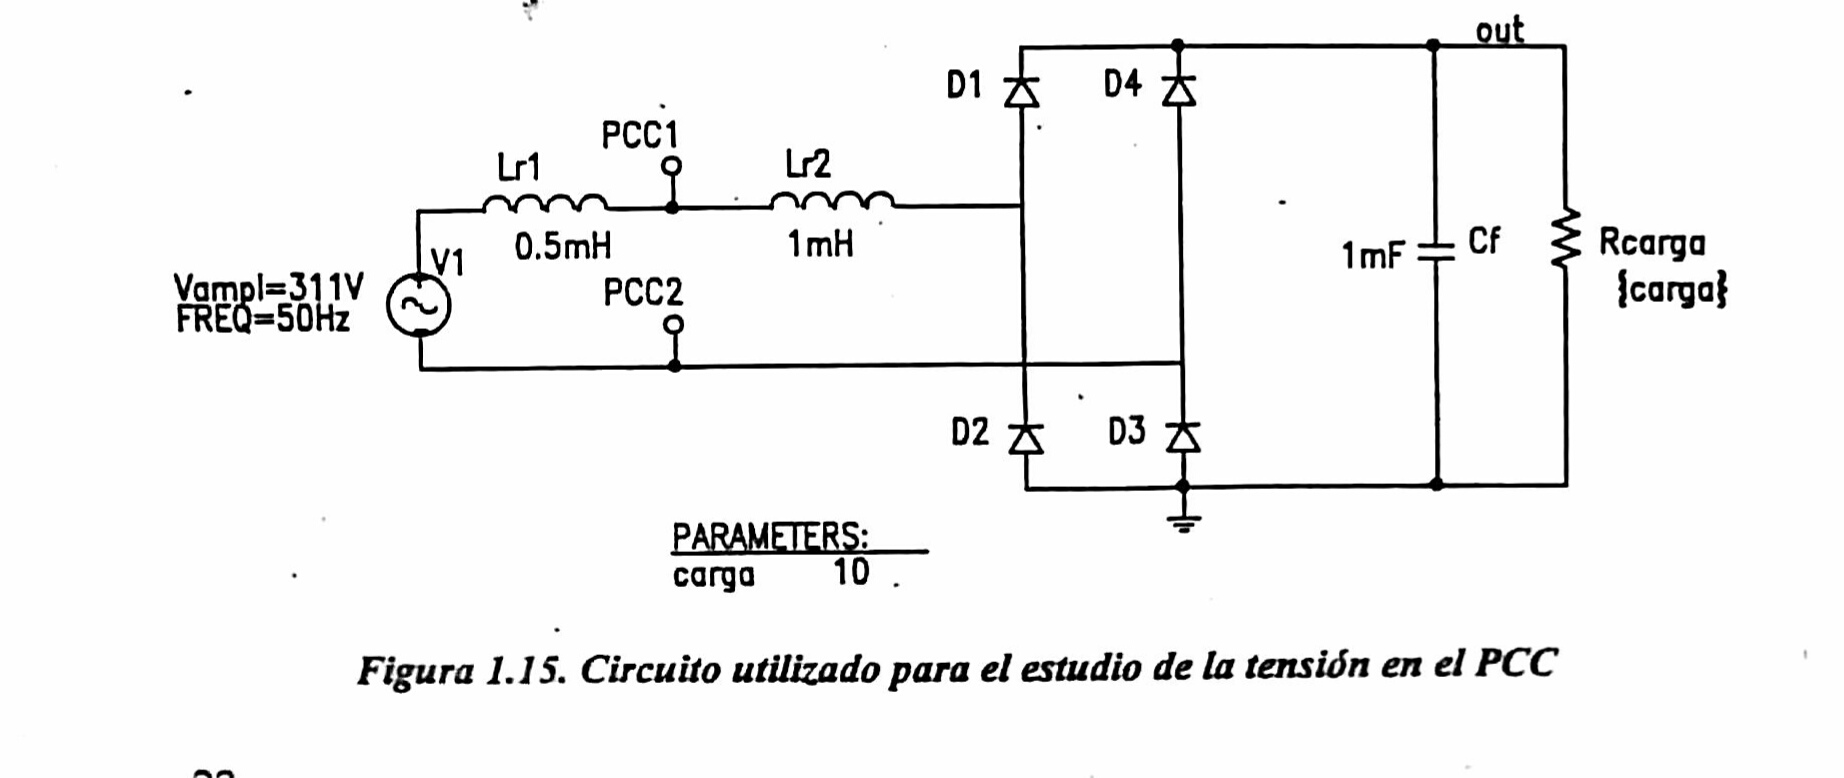
\includegraphics[width=7cm]{Escritorio/Practica 1/h.jpg}
 \caption{Estudio de la tension en PCC}
 \end{figure}
 
 Este circuito, muestra lo mismo que el anterior, solo que este tiene el doble de induccion, esto deja ver como entre esas conexiones hay una distorcion a la hora de generar la onda, conectada la punta de prueba a la primera bobina.
 
 \item \textbf{Rectificador Monofasico Duplicacion de Tension:}
 \begin{figure}[hbtp]
 \centering
 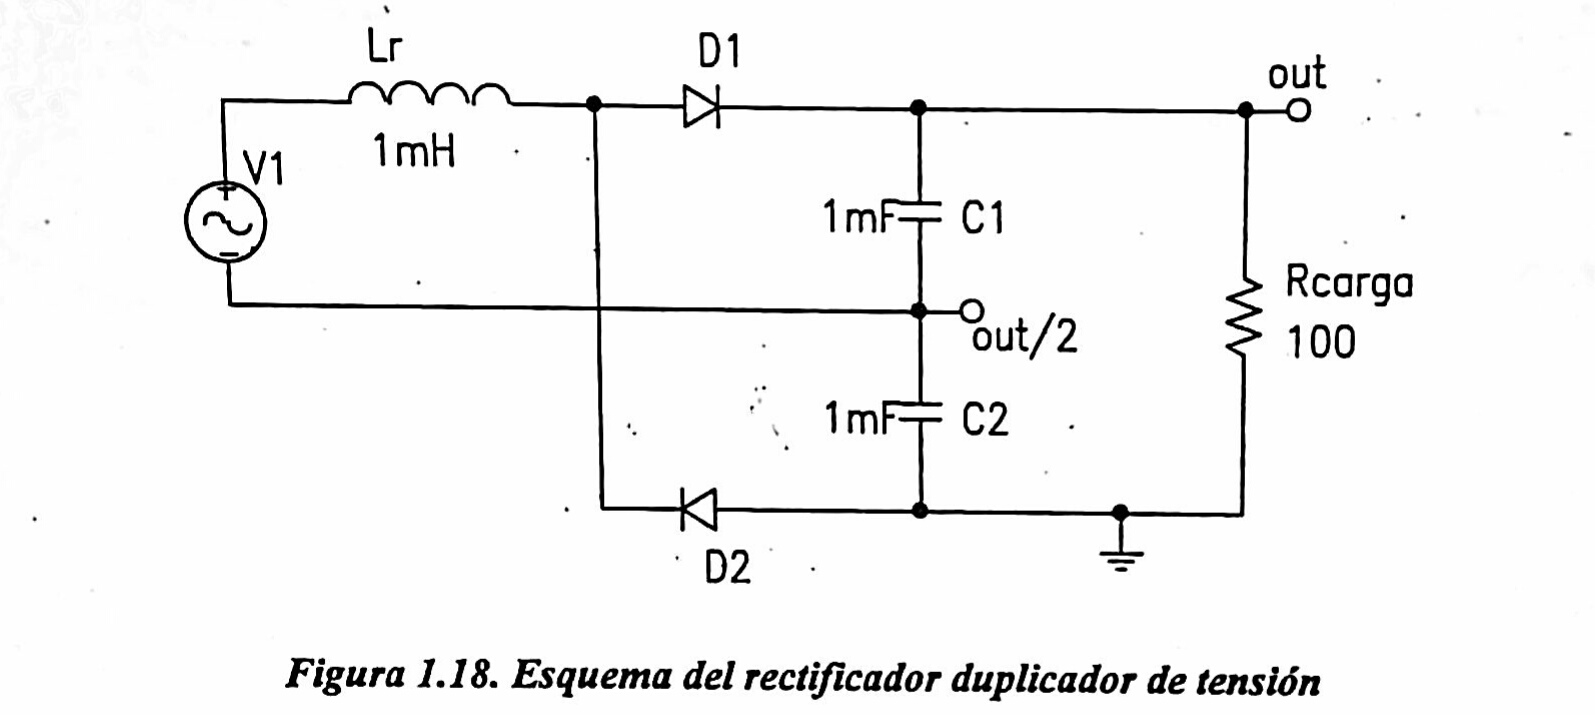
\includegraphics[width=7cm]{Escritorio/Practica 1/i.jpg}
 \caption{Rectificador duplicador de tension}
 \end{figure}
 

 El diagrama de este punto, es sencillo de ver, ya que no tiene ningun componente nuevo, simplemente se agregaron dos capacitores, que como el nombre del sistema o circuito te deja ver, es un duplicador de tension, dada las conexiones que se muestran en el diagrama.\\
 Vemos conectado el primer diodo norrmalmente, lo cual este deja que entre la corriente y este la dirige de forma directa, a la resistencia, la cual cumple su funcion que es la de regular la corriente que hace pasar por el inductor, y el diodo, la otra pata de la resistencia va directo conectado al otro diodo, que hace la misma funcion que el otro diodo, ya que deja entrar y regula la corriente que va conectado al inductor directamente. Al repetir este ciclo, lo que hace es que los capacitores que estan conectados a mitad del circuito, agarren toda la corriente y recaiga toda la tension por esos dos capacitores, ya que tambien se ve que la entrada negativa de la fuente alterna, va conectado de forma directa a la mitad de los dos capacitores, y es lo que hace un bucle, repite dicha tarea cada cierto tiempo que estos dos capacitores se descarguen, y cuando estos se cargan, generan el duplicador de tension, que eso es lo que le da el sentido a las conexion monofasica, de un sistema de distribucion de energia.
 
 \item \textbf{Efectos de los Rectificadores Monofasicos en lineas Trifasicas}
\begin{figure}[hbtp]
\centering
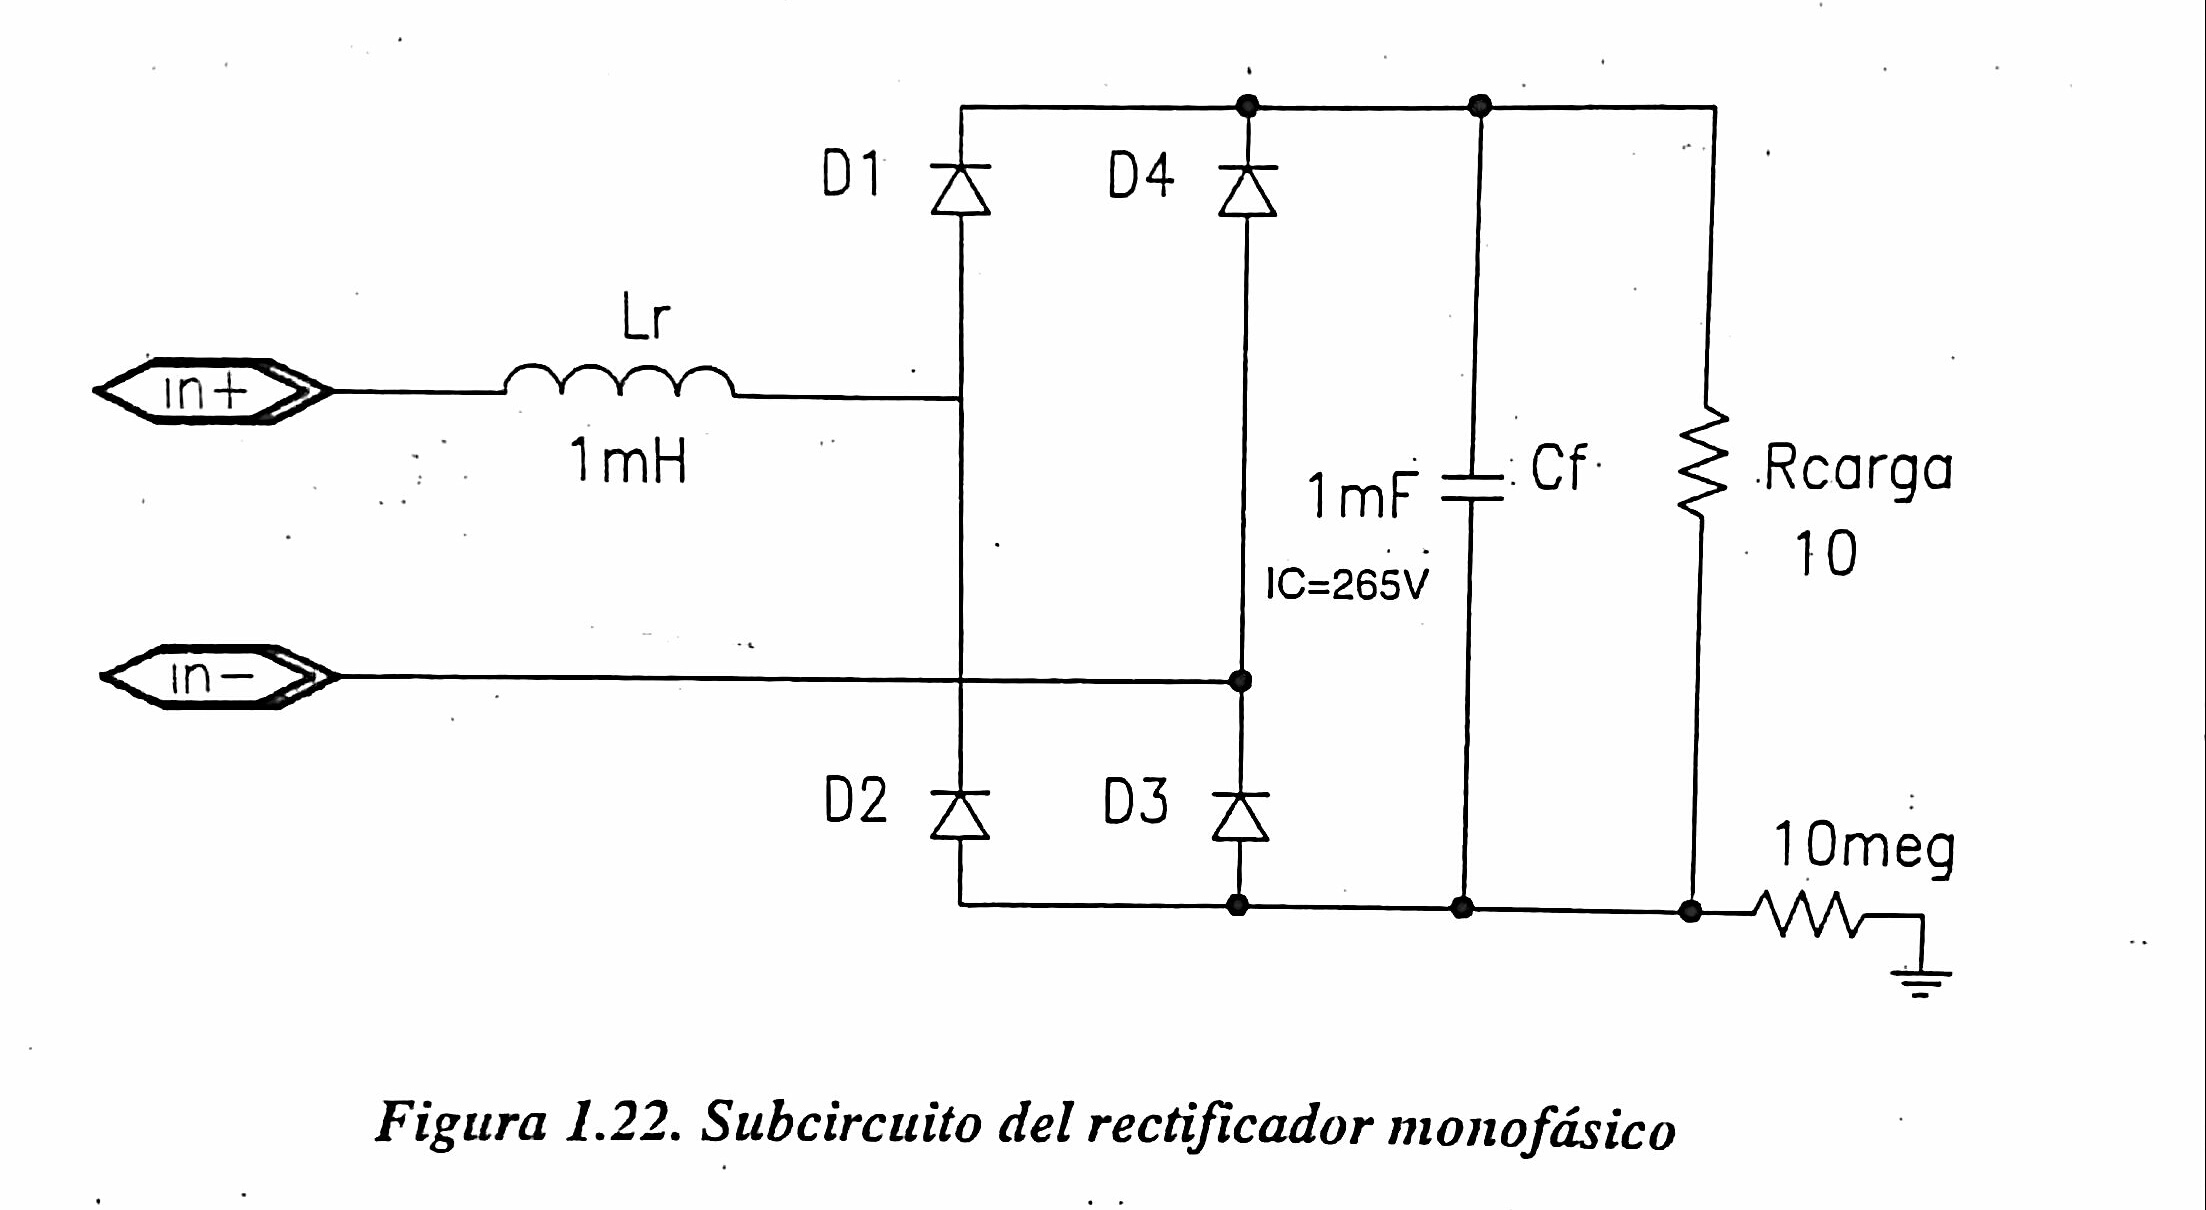
\includegraphics[width=7cm]{Escritorio/Practica 1/j.jpg}
\caption{Rectificadores monofasicos en lineas trifasicas}
\end{figure}

 
 En esta parte, vemos como una sola fuente de poder(alterna), acopla lo que vendria siendo en un puente de 4 diodos, la fuente de poder trifasica, al estar conectada la fuente tanto la parte positiva, a la parte de arriba de los 4 diodos, y la parte negativa al otro cruce de los dos diodos, esto para que los diodos hagan una caida de voltaje, hasta llegar a el capacitor, donde nuevamente, esta cumplira su funcion que la corriente de los diodos, le esten dando y este genera en ondas, que mas adelante se estara viendo en los resultados.\\
 Como se aprecia, la resistencia que esta en paralelo con el capacitor, cumple una funcion eficiente, al ser este el regulador en el paso de corriente despues de que el capacitor se termine de cargar, o en otro caso se descargue, para ver como este se comporta, y este es conectado siempre a tierra, para que las ondas no se estropien, y cumpla lo que estamos viendo, que seria el de tener la fuente alterna, en constante cambio de ondas.\\
 Las puntas de prueba van tanto al OUT, esto  para que se aprecie como en si, aunque este en esa posicion, no esta sin corriente, ni voltaje, sino que ahi mismo sigue trabajando, y de que manera dando ondas senoidales completas, las cuales, se ve en el circuito que todo paso de corriente es para algo, y en este caso para un cambio constante de ondas.\\
 Formula utilizada:\\
 \emph{fourier}
 $$ i_{neutro}(rms)= \sqrt{\sum_{h=3,9,15}} 3* i_{Lh}= 3* i_{L3}$$
 
 \item \textbf{Rectificadores Trifasicos:}
\begin{figure}[hbtp]
\centering
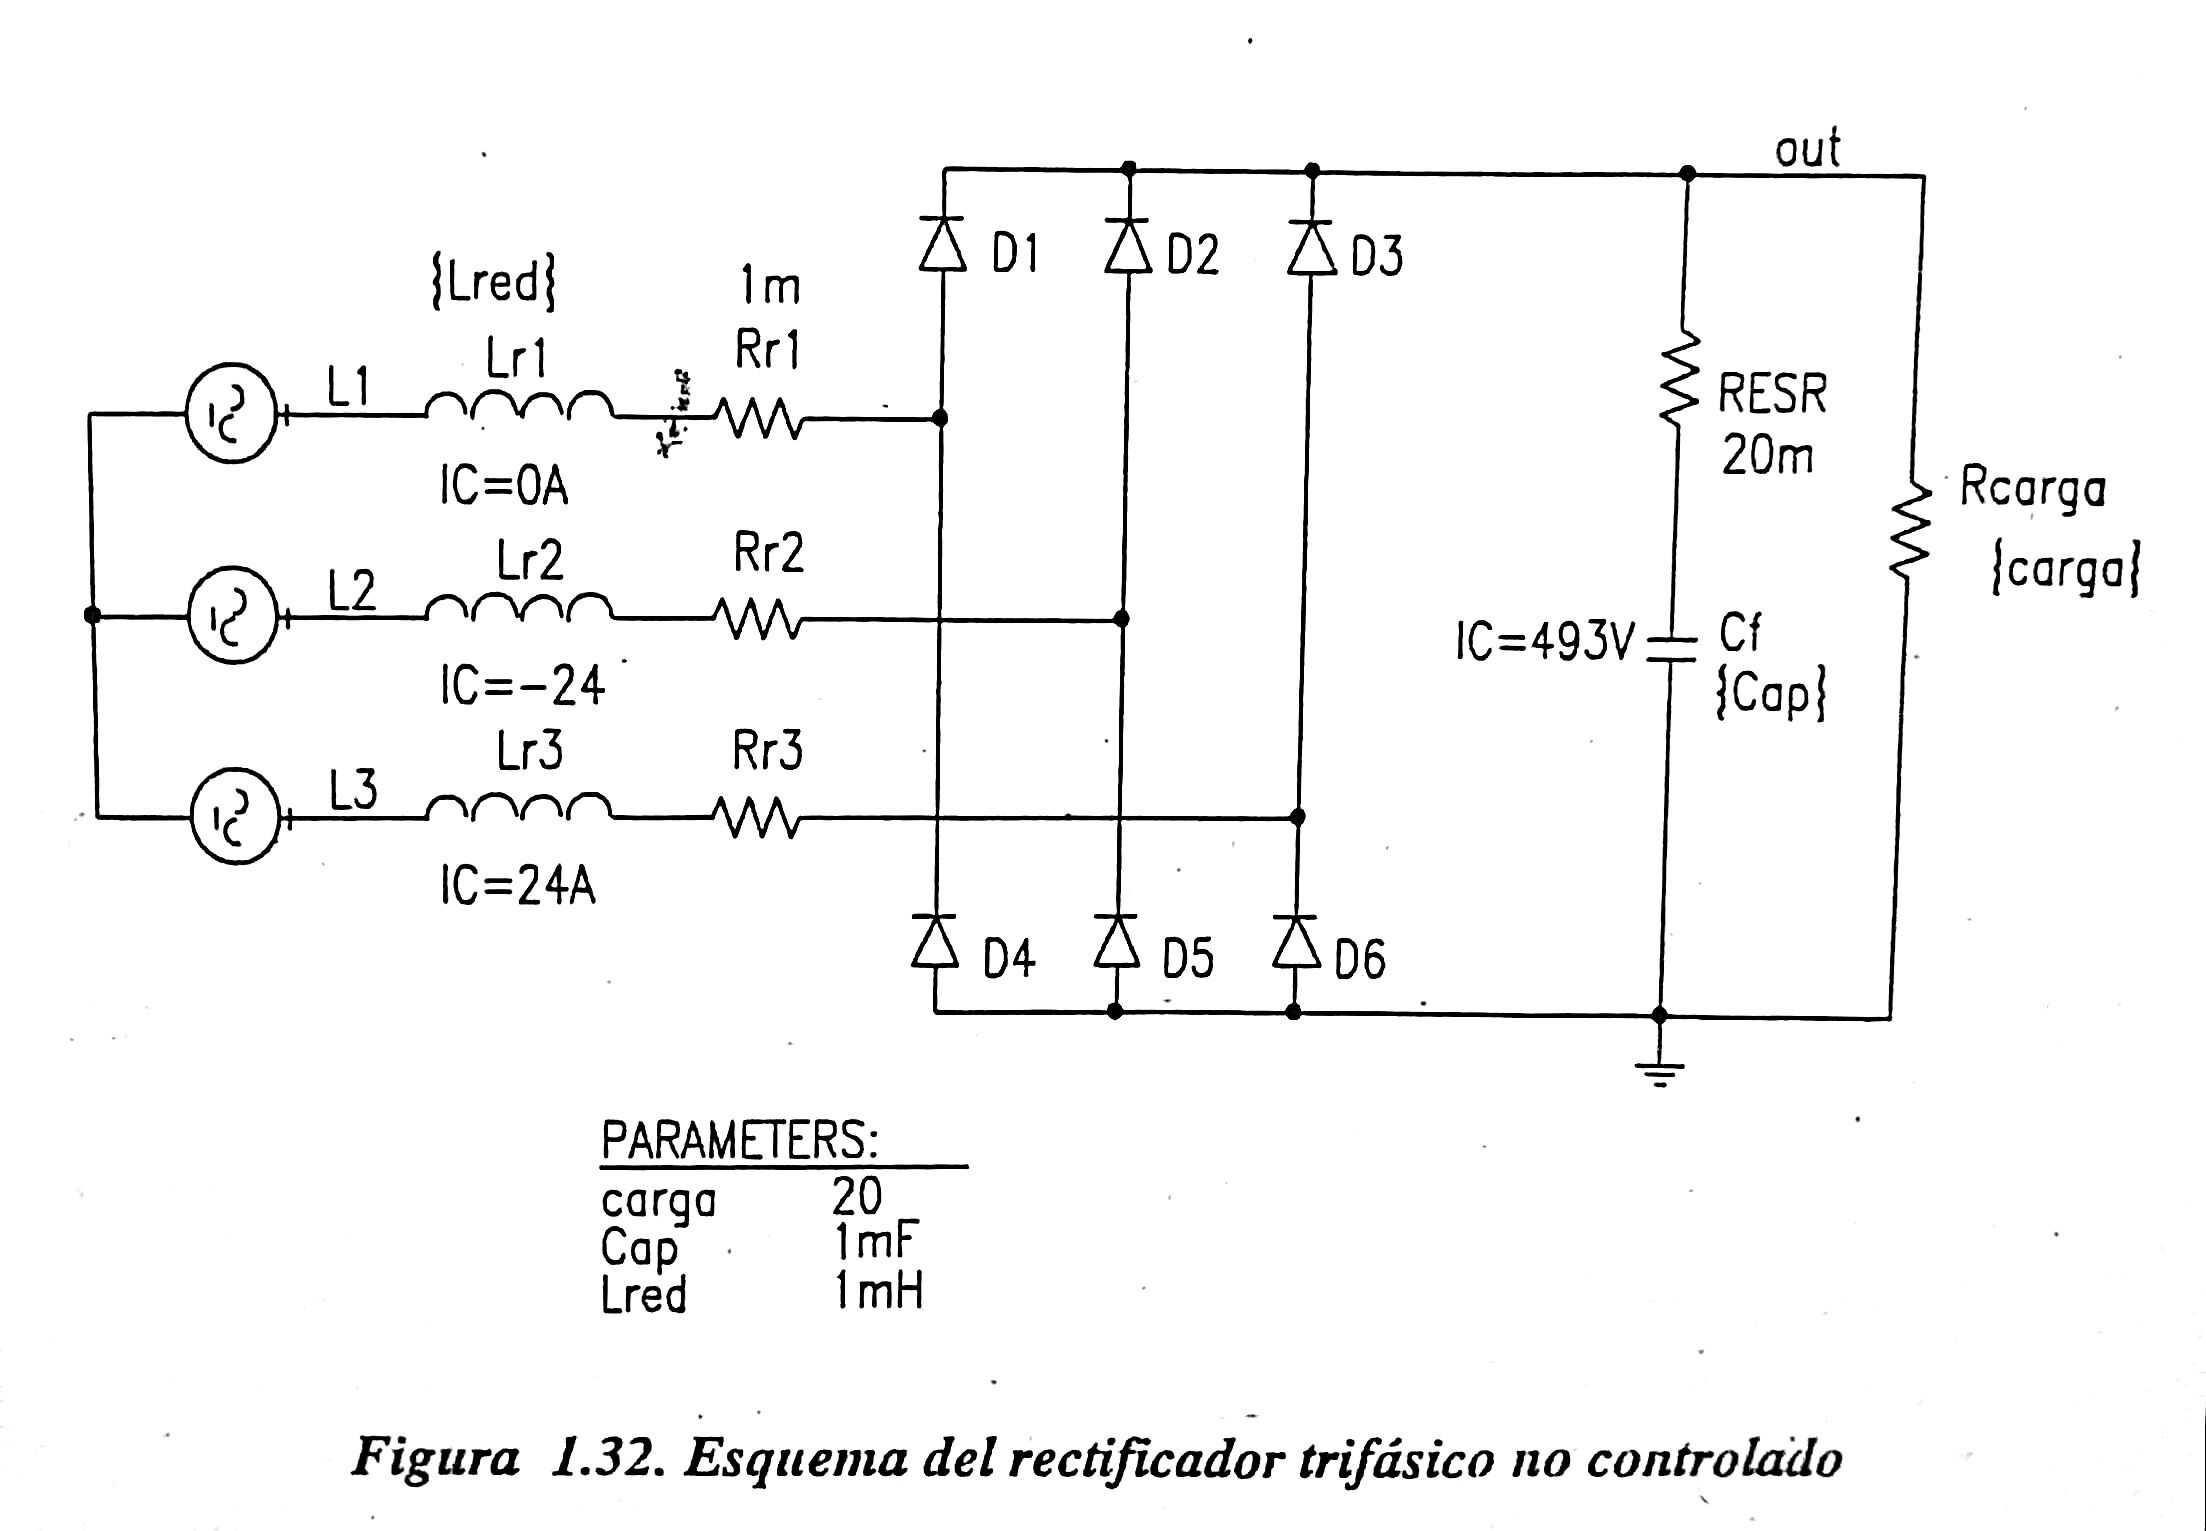
\includegraphics[width=7cm]{Escritorio/Practica 1/a.jpg}
\caption{Rectificador trifasico no controlado}
\end{figure}

  
En este diagrama, lo que se simulo y se armo, es para ver la funcion de tres fuentes de poder, todas alternas, conectadas entre si, como estas van conectadas a cada par de diodos, que se muestran tambien en el diagrama. Para poder ver de que manera se comporta cada fuente, y como entre ellas se juntan, tanto la fuente 1, como la fuente 3, estan conectadas directamente, sus salidas, y la salida del voltaje 2, esta conectada a las dos fuentes anteriores.
Vinedo el mismo sistema que en los otros casos, en donde el capacitor hace su funcion, en este caso sus ondas senoidales, nos dan el visto de como 6 diodos rectificadores trabajan entre si, dirigiendo la corriente por dos puntos, en el anodo y el catodo, siendo este tambien proporcionado por un inductor.\\
El inductor conectado de forma en serie, a la resistencia, es el que crea un campo magnetico sobre el circuito, lo que hace disparar su corriente y darle al circuito, una base extra de corriente, y en si sus funciones dando dnetro, de la rsistencia que va conectada tambien de forma en serie con el capacitor y este en si, regula tanto esa resistencia, la llegada de la corriente al anodo del capacitor, lo que hace la generacion de sus ondas, y el mismo caso que el circuito anterior, donde hay una resistencia en paralelo, tanto con la resistencia y el capacitor. 
  
 \begin{figure}[hbtp]
 \centering
 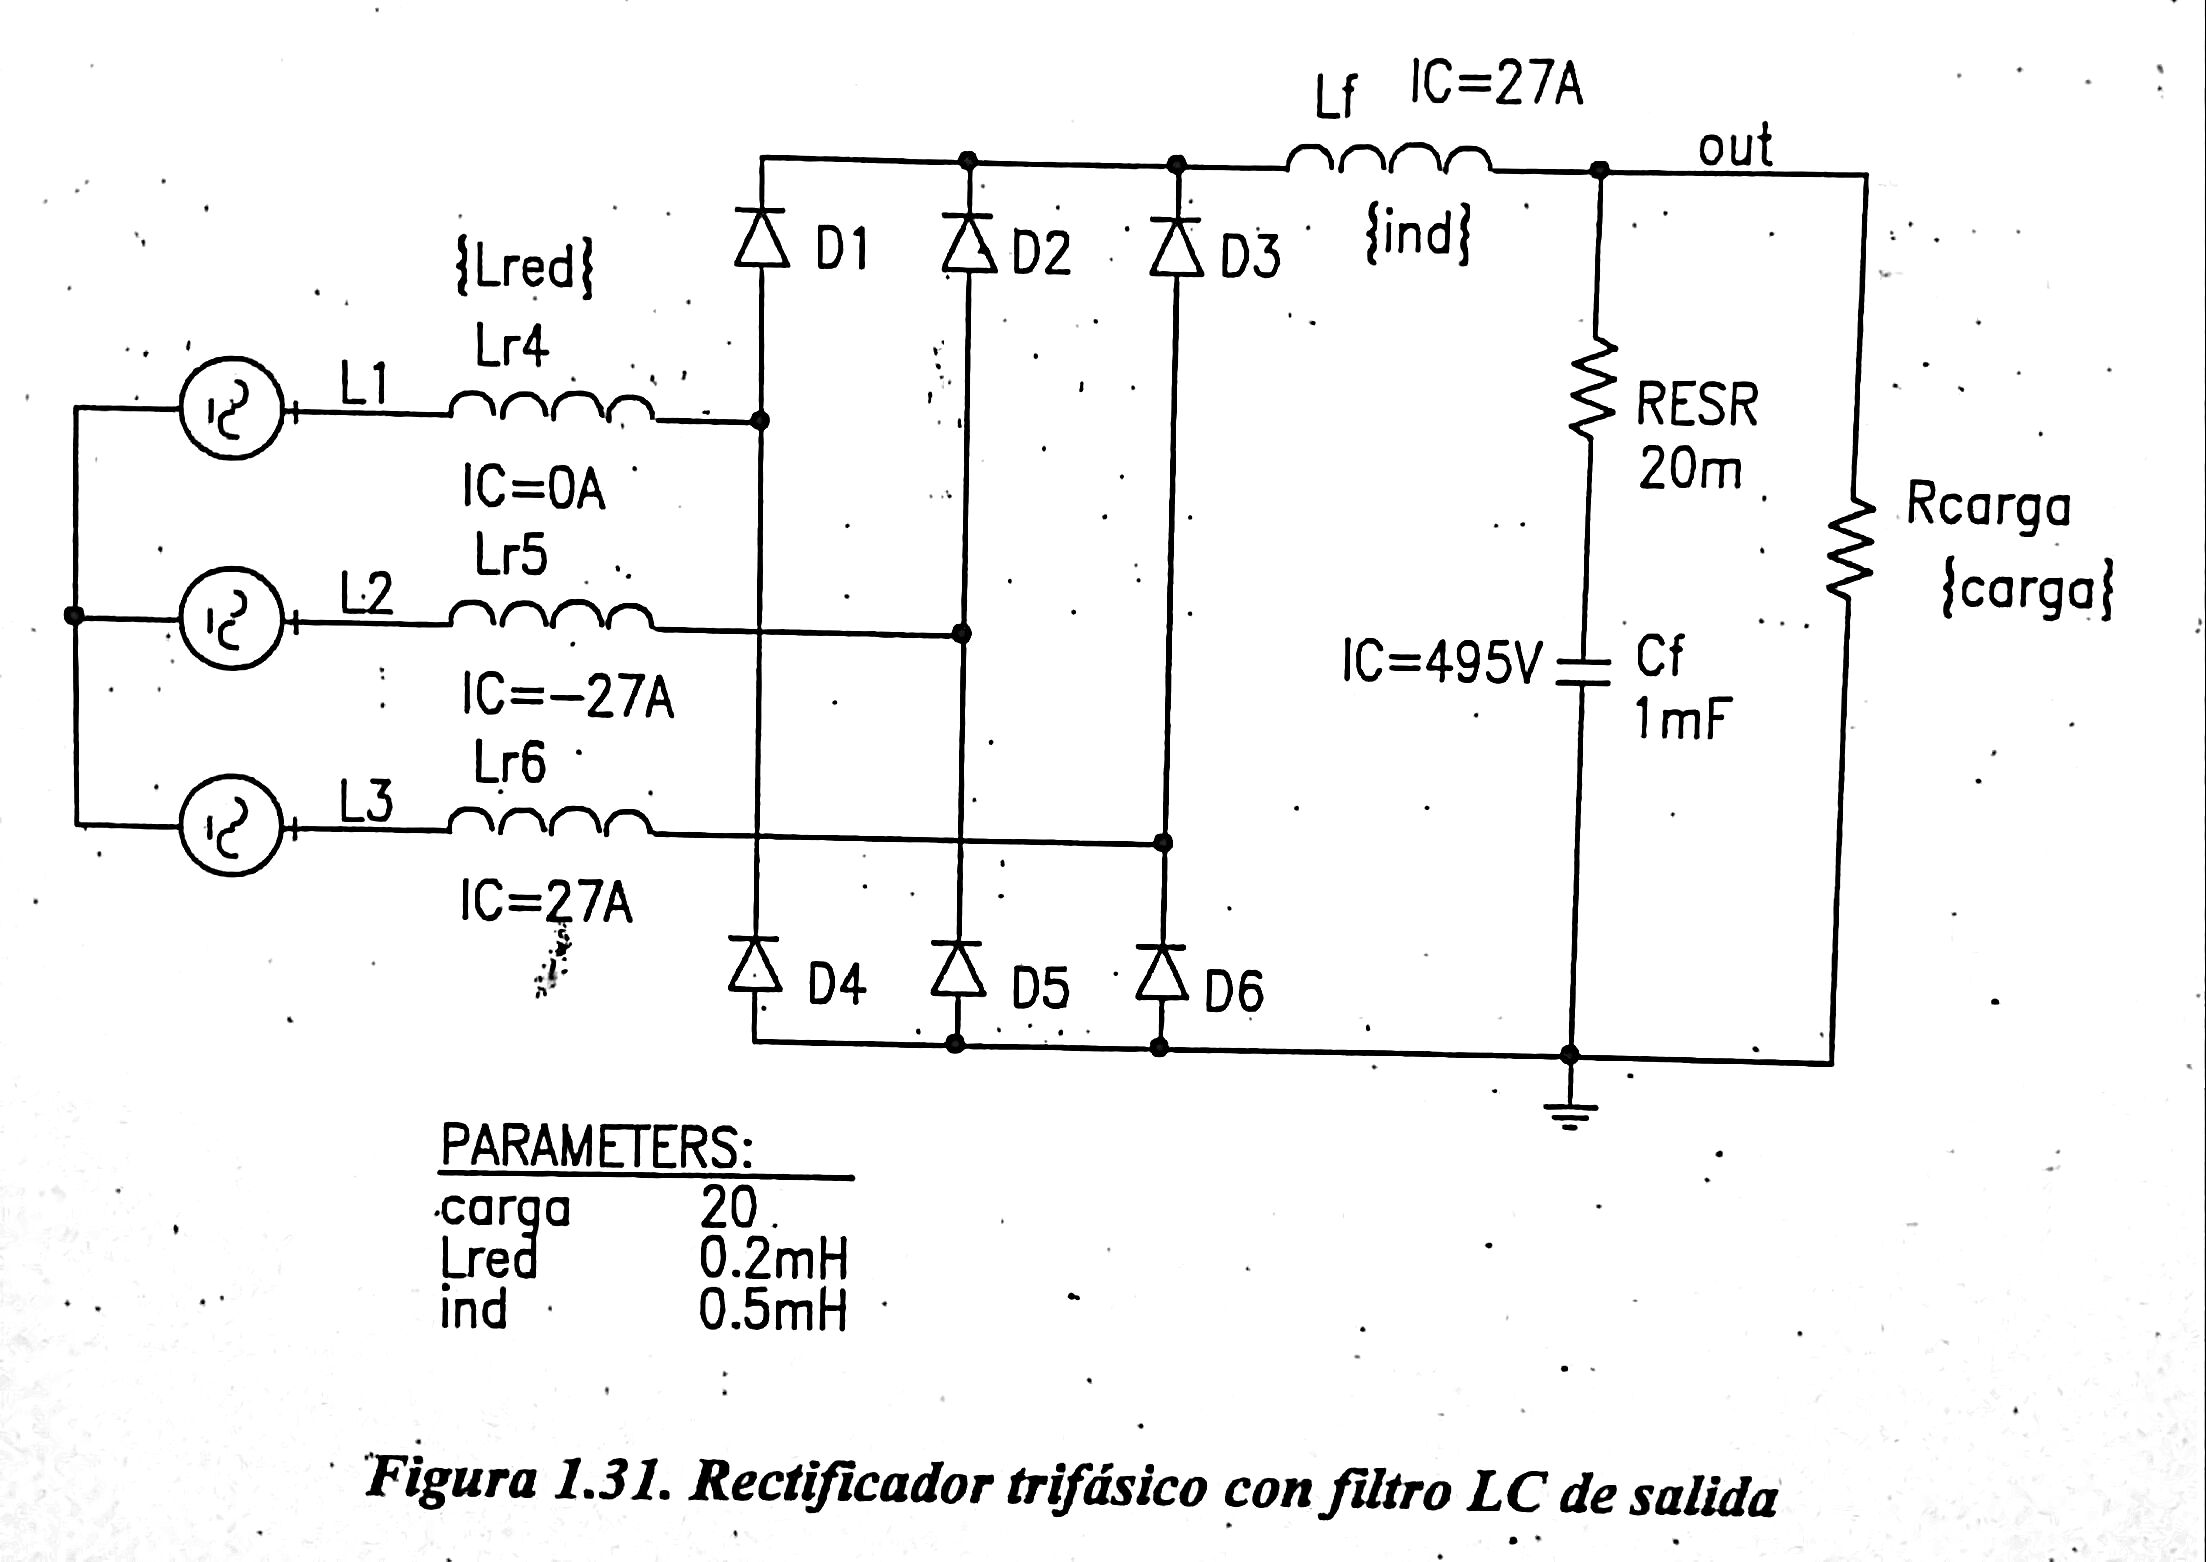
\includegraphics[width=7cm]{Escritorio/Practica 1/b.jpg}
 \caption{Rectificador trifasico con filtro LC de salida}
 \end{figure}
 
  
Ahora en este diagrama, se ve lo mismo que en el caso anterior, con la diferencia de que, hay una bobina entre todos los diodos, y el capacitor, esto hace que la inductancia del componente, se comporte de otra forma, cambiando las ondas del capacitor, y de todo el circuito en si, se declara que el haber puesto en esos puntos interfieriendo entre los diodos, las fuentes y por otra parte el capacitor, y sus respectivas resistencias, hace que el flujo de corriente cambie drasticamente, dando lo ya dicho, generaciones de ondas recortadas.\\
En si, en otra contraparte, se estuvo manejando el voltaje en rms, que nos deja apreciar el valor real que estan manejando cada onda generada, y como de ello se puede ver reflejada la diferencia entre el voltaje de la red, y del voltaje rms, asi como el de los componentes conectados en todo el circuito.
  
  \item \textbf{Efecto de las inductancias de red sobre conmutacion de Corriente:}
 \begin{figure}[hbtp]
 \centering
 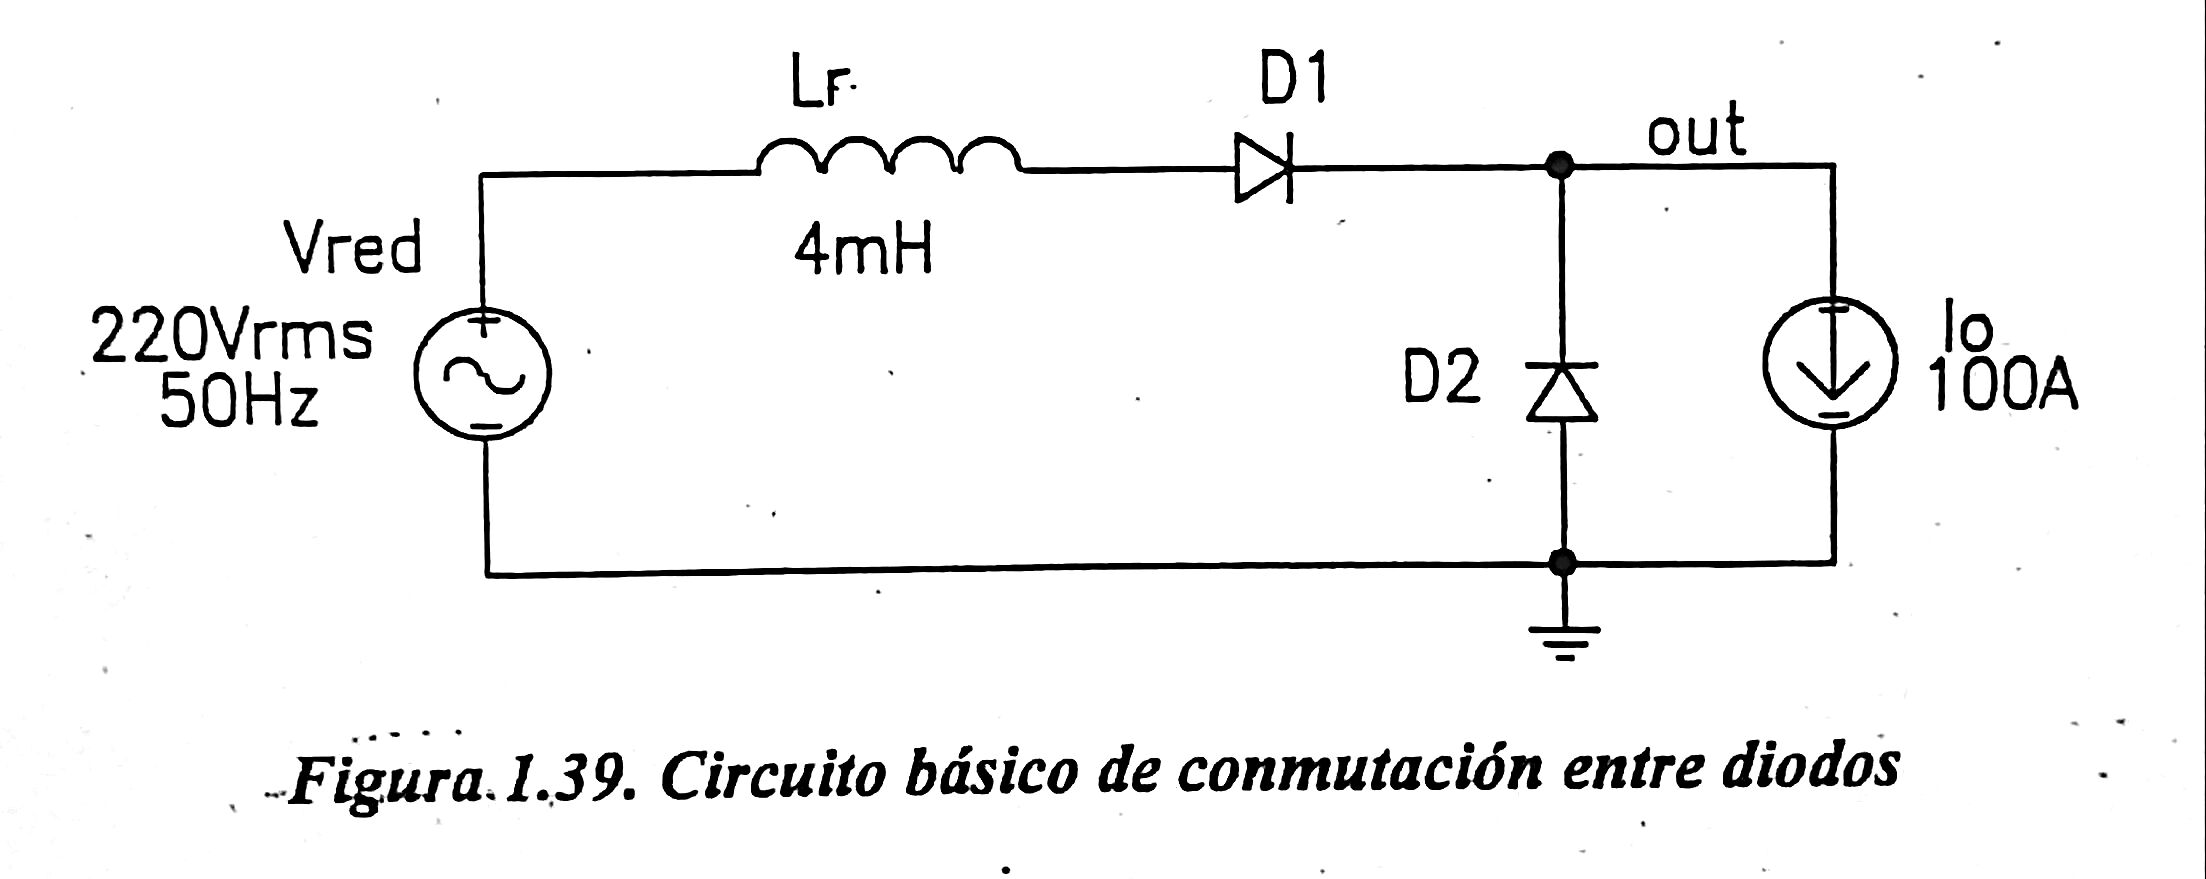
\includegraphics[width=7cm]{Escritorio/Practica 1/c.jpg}
 \caption{Conmutacion basica entre diodos}
 \end{figure}
 
 Formula utilizada:\\
 \emph{fourier}
  $$ P_{condensador}= R{ESR}* I_{c}(RMS)$$
  
Los diagramas del apartado 1.7, son en si enfocados, mas a la inductores, y como de ello se deriva una corriente diferente, dejando en  temas mas relevantes, como este componente.\\
En el primer diagrama se ve una conexion simple y basica, dandonos en el diagrama dos diodos, una bobina y una fuente de corriente, el cual deja ver como entre una fuente de voltaje alterna, y una fuente de corriente, hay diferencias, generando el pause, entre los diodos, y como estos en ciertos puntos bolquean el paso de corriente, generando ondas, con recorte de voltaje, y corriente en un cierto parametro de la simulacion, y como este deja fluir en cierto punto, su voltaje sube y baja, y hay una buena rectificacion entre estos puntos. Demostrando.\\
Formula utilizada:\\
 \emph{fourier}
$$ V_{o}= \frac{2w*L{r}}{pi}* i{o} $$
 
 \begin{figure}[hbtp]
 \centering
 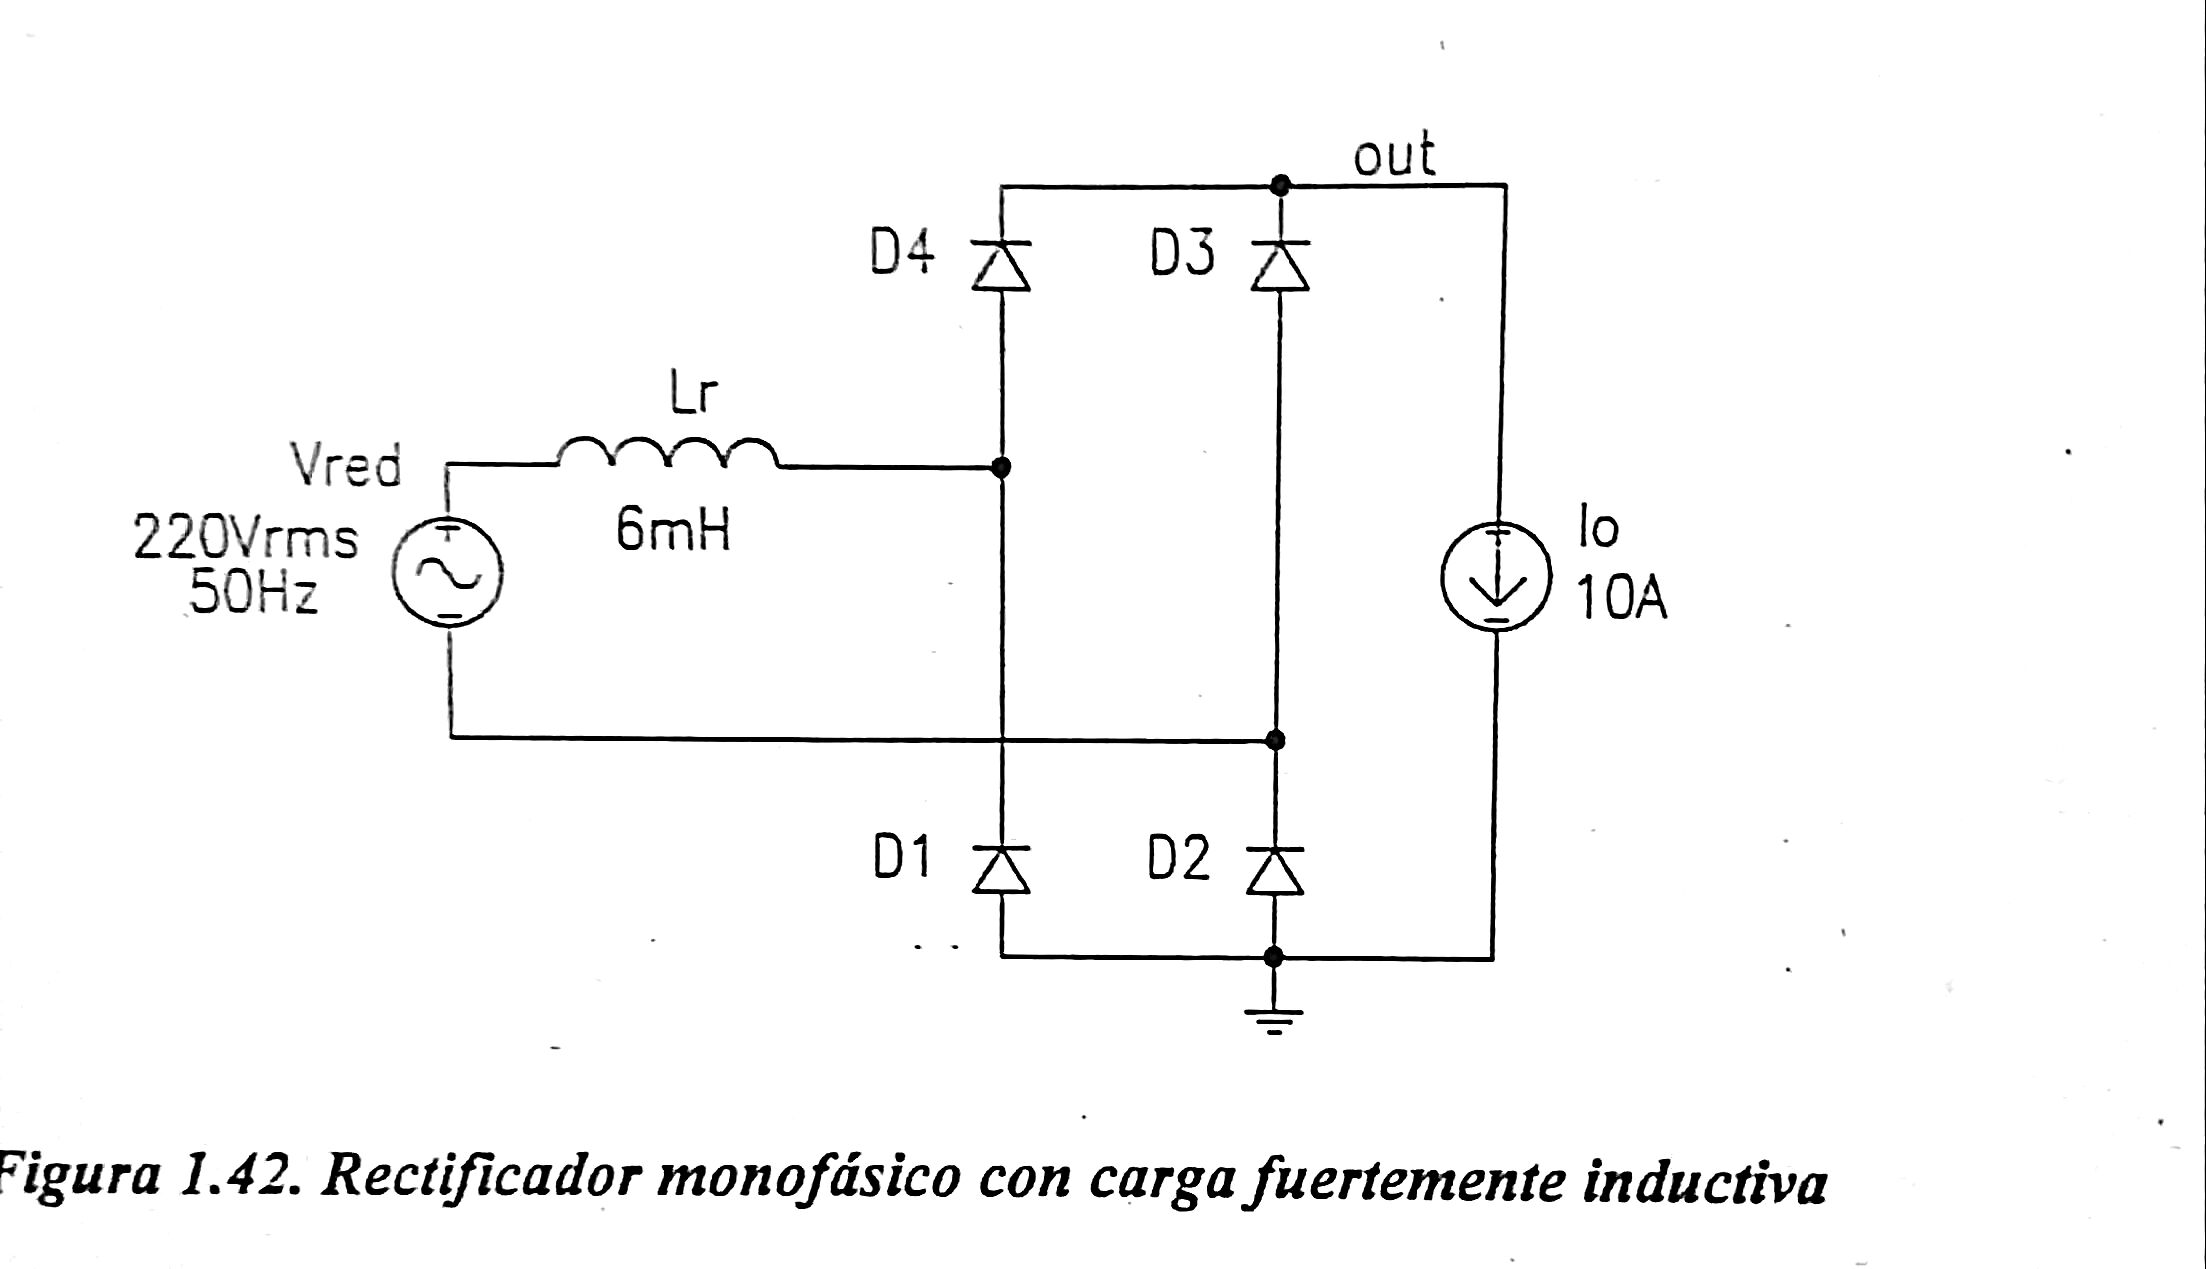
\includegraphics[width=7cm]{Escritorio/Practica 1/d.jpg}
 \caption{Rectificador monofasico con carga inductiva fuerte}
 \end{figure}
 
 
Se puede apreciar, el valor de inductancia que hay en este circuito, lo que hace en si, sean mas bruscas las ondas, pero en si no hay mucho cambio solo que el campo magnetico que genera este inductor es mas amplio, lo que hace que los diodos reciban mas corriente y esto se ve en la generacion de ondas.
 
\begin{figure}[hbtp]
\centering
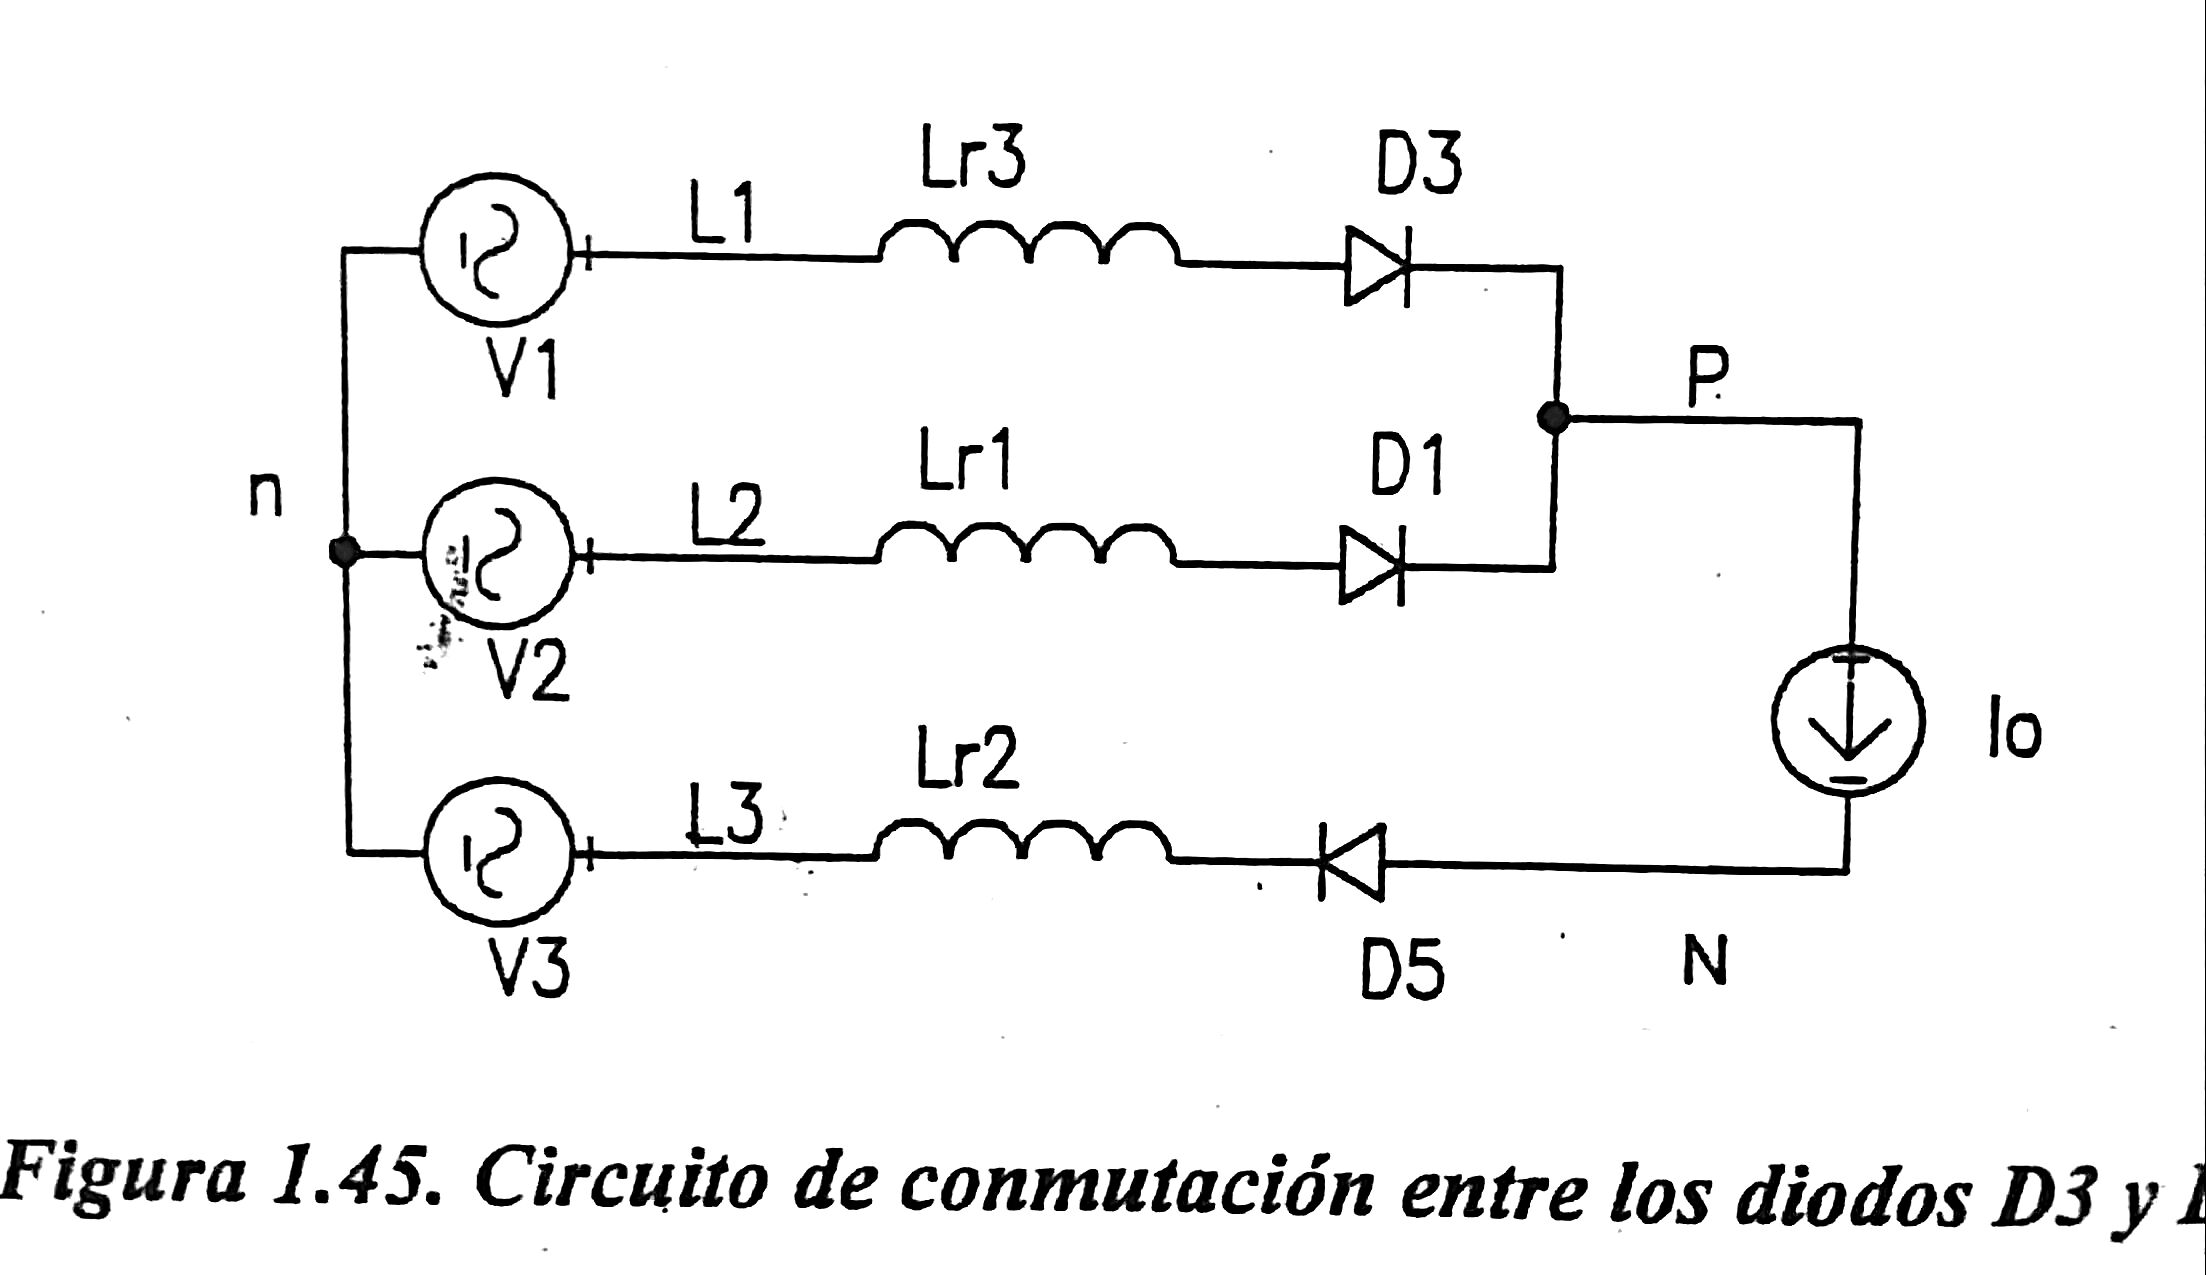
\includegraphics[width=7cm]{Escritorio/Practica 1/e.jpg}
\caption{Circuito de conmutacion entre diodos}
\end{figure}

 
En este ultimo diagrama, se ve la comprobacion de como entre diodos se comunica la corriente, que circula por todo el circuito, hay en si tres fuentes de voltaje alteno, como entre ellos hay dos que estan conectados de forma igual, y otro que esta conectado de forma inversa, que seria el de la fuente 3, la cual hace que la circulacion de corriente, por los dos primeros puntos, se tope con el diodo 3, en el cual tambien se ve un paro de onda, y una subida, parecido al circuito anterior, con la diferencia que este tiene mas fuentes de por medio entre si.\\

Formula utilizada:\\
 \emph{fourier}
 $$ V_{PN}= V_{pn}- V_{Nn} $$
 $$ V_{o}= \frac{3}{pi}* w* L_{r}* I_{o} $$

Nota: En todos los casos, de este punto, se utilizo una fuente de corriente, que hace mas facil el flujo de corriente.

\end{enumerate}

\section{Resultados:}

\begin{figure}[hbtp]
\centering
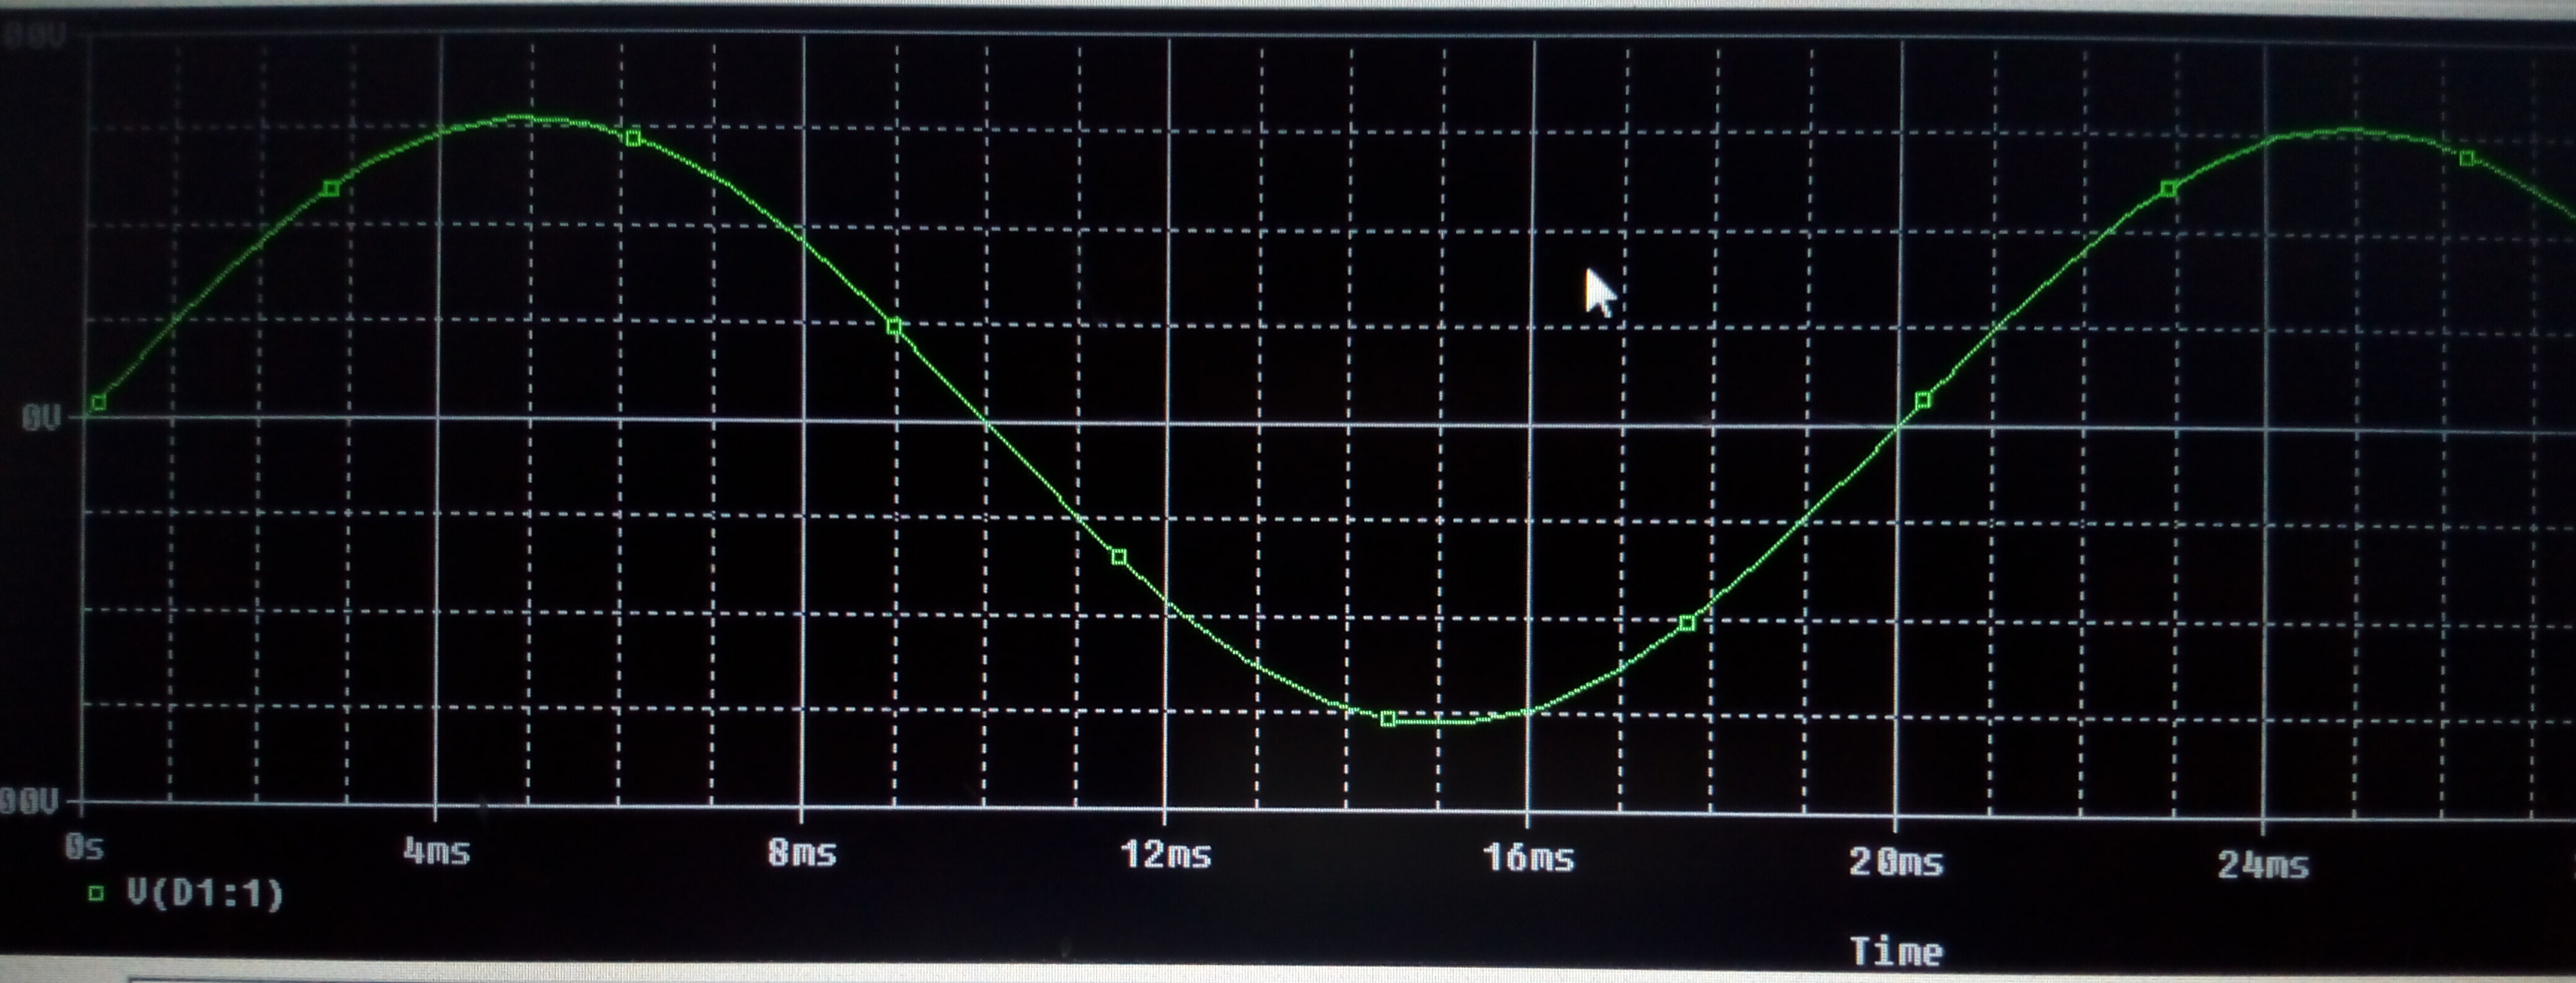
\includegraphics[width=8cm]{Escritorio/Practica 1/1.jpg}
\caption{V(D1), Rectificacion de media onda con carga RL}
\end{figure}


\begin{figure}[hbtp]
\centering
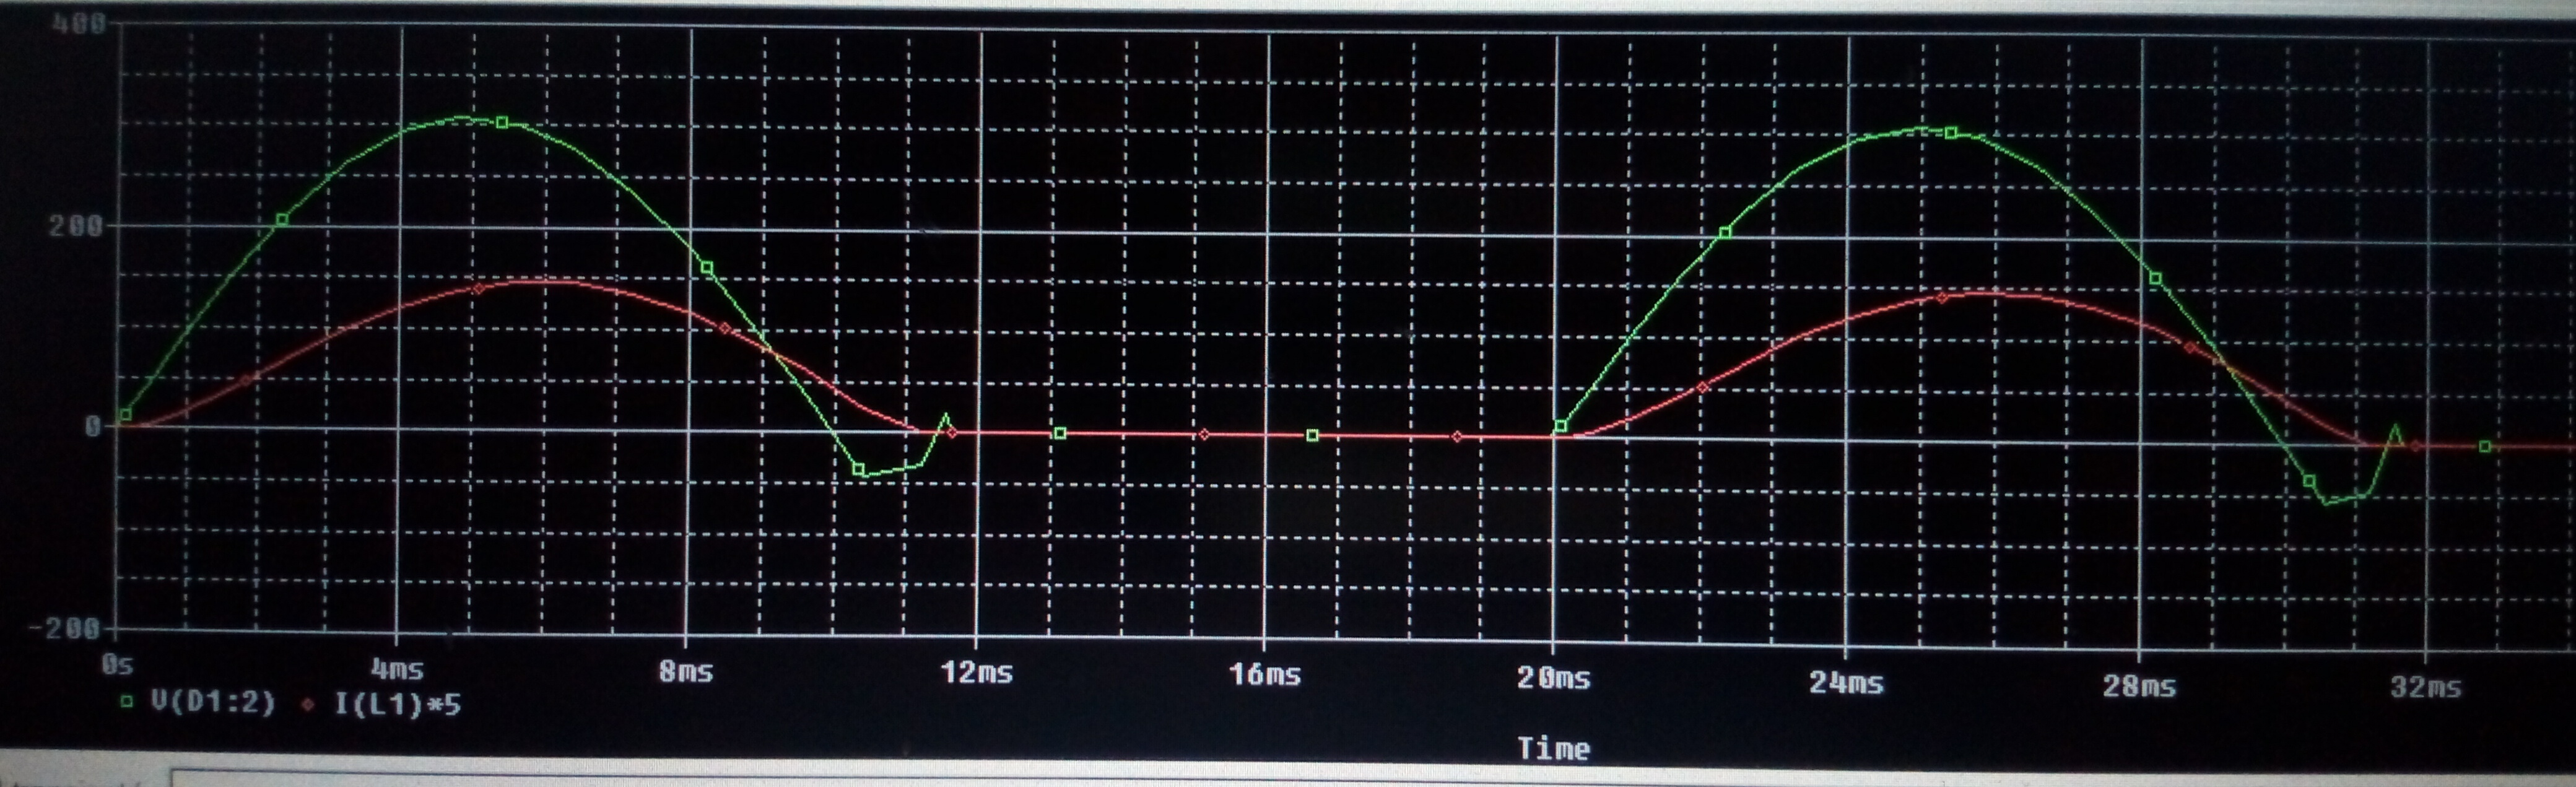
\includegraphics[width=8cm]{Escritorio/Practica 1/2.jpg}
\caption{V(D2, Rectificador de media onda.), I(L1)*5}
\end{figure}


\begin{figure}[hbtp]
\centering
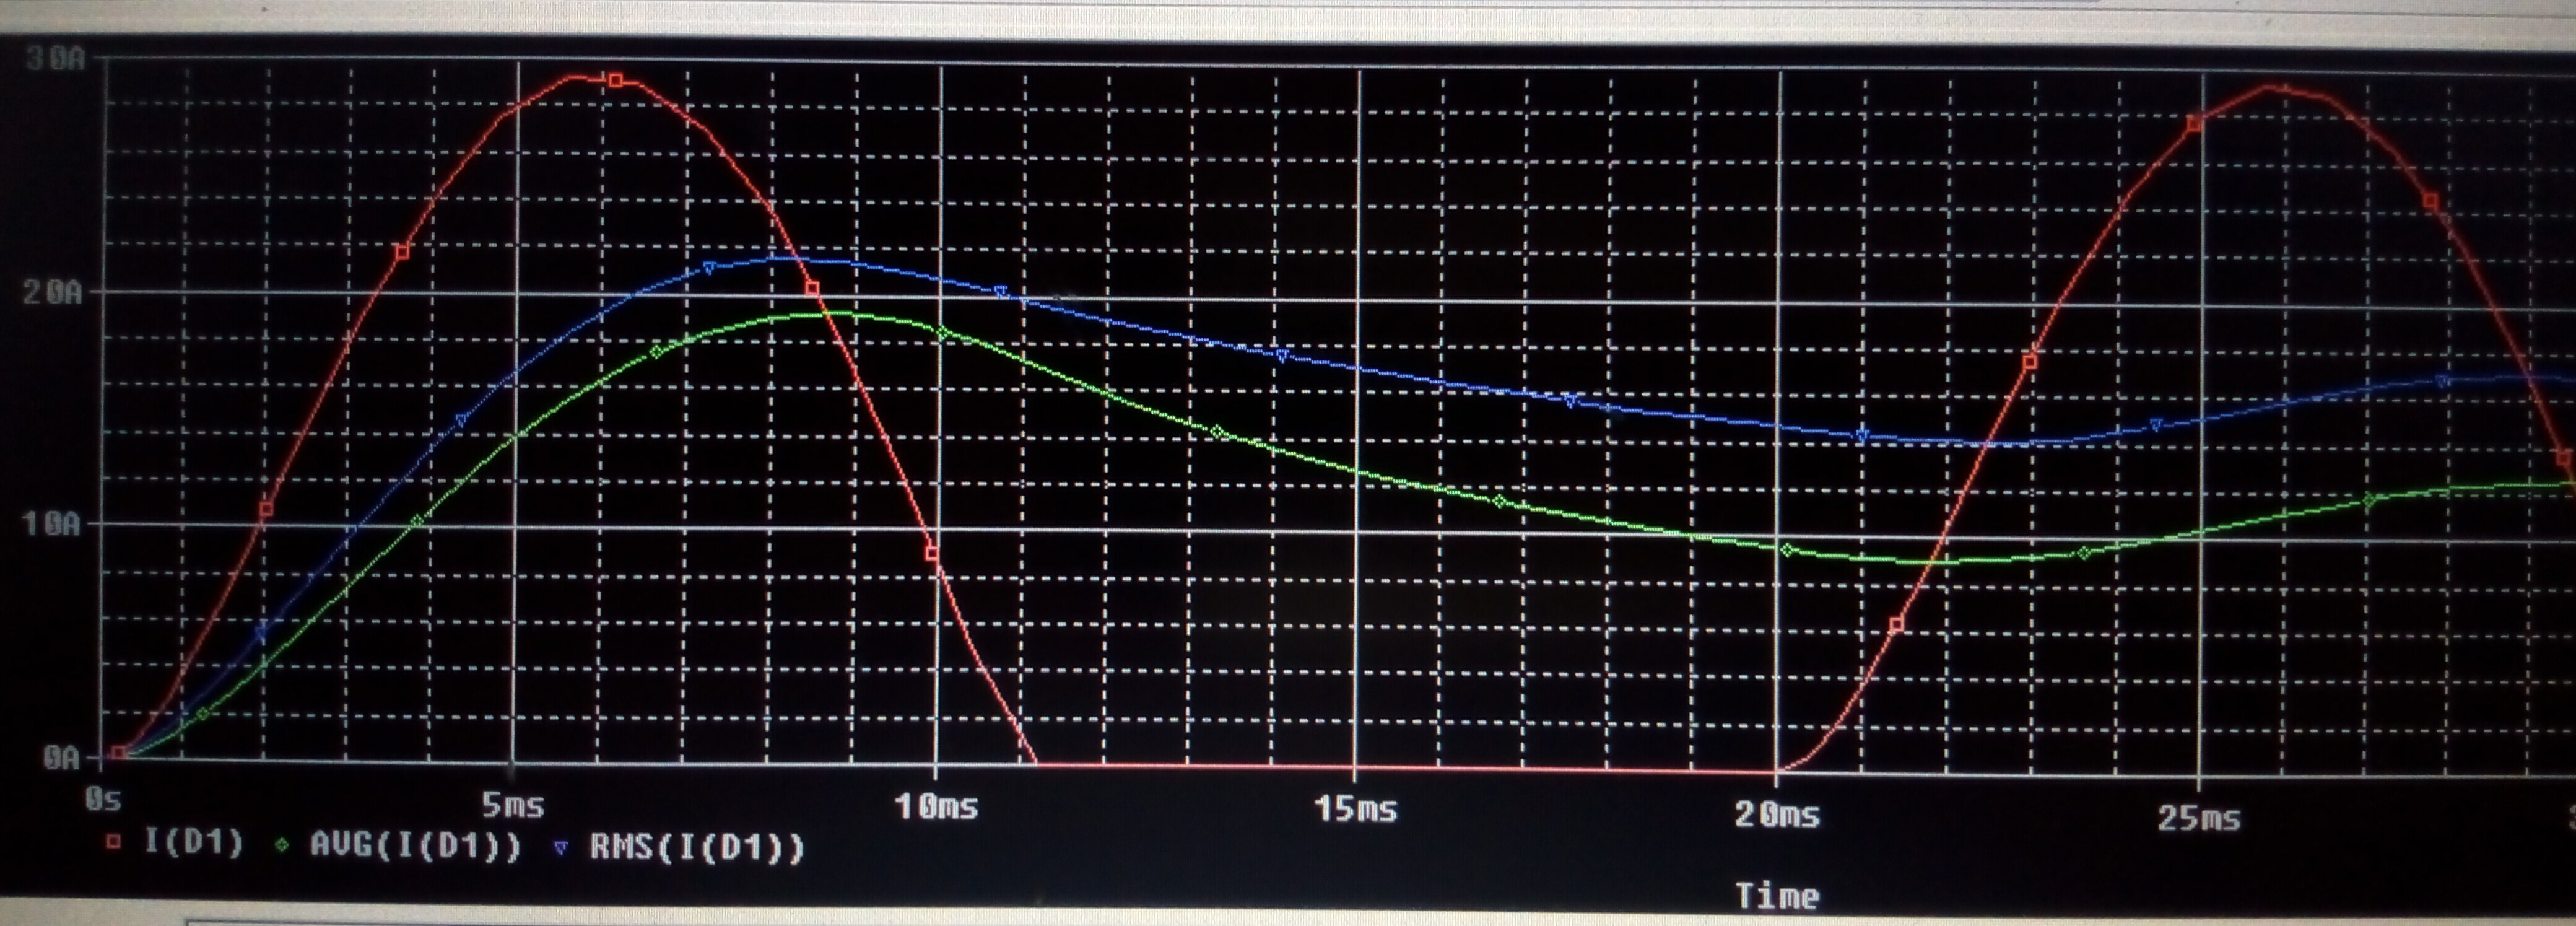
\includegraphics[width=8cm]{Escritorio/Practica 1/3.jpg}
\caption{I(D1)}
\end{figure}

\begin{figure}[hbtp]
\centering
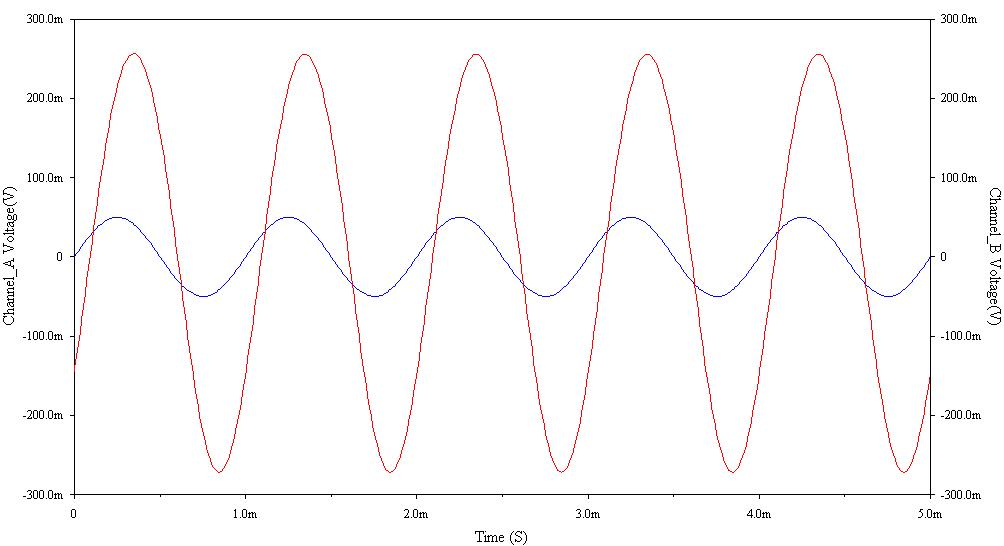
\includegraphics[width=8cm]{Escritorio/Practica 1/4.jpg}
\caption{V(D1:1)-V(D1:2)}
\end{figure}


\begin{figure}[hbtp]
\centering
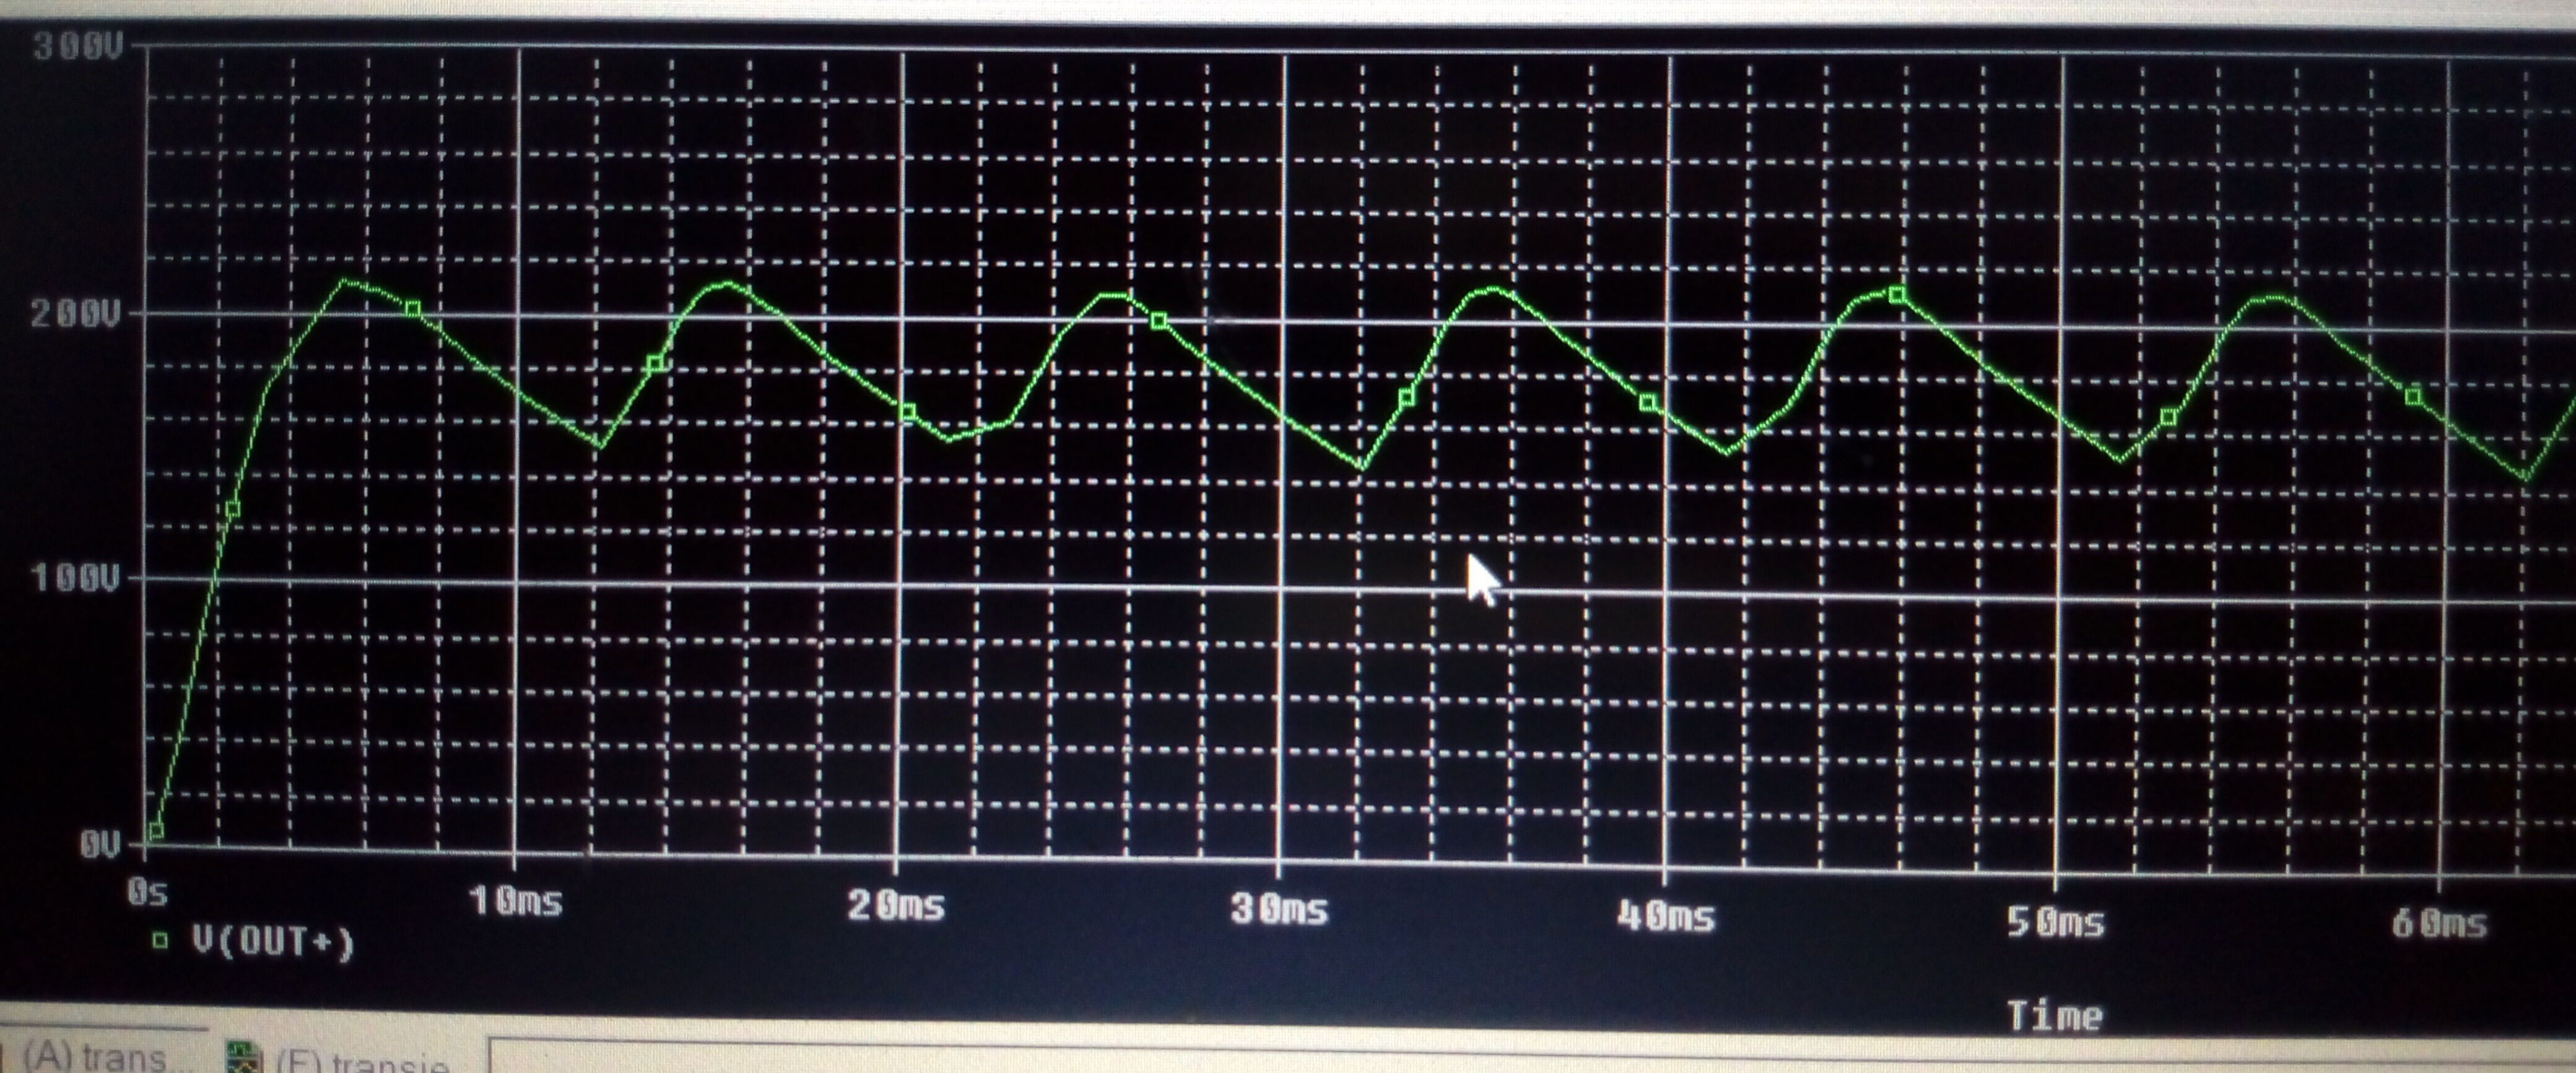
\includegraphics[width=8cm]{Escritorio/Practica 1/5.jpg}
\caption{V(OUT, rectificador monofasico en fuente), R=10}
\end{figure}

\begin{figure}[hbtp]
\centering
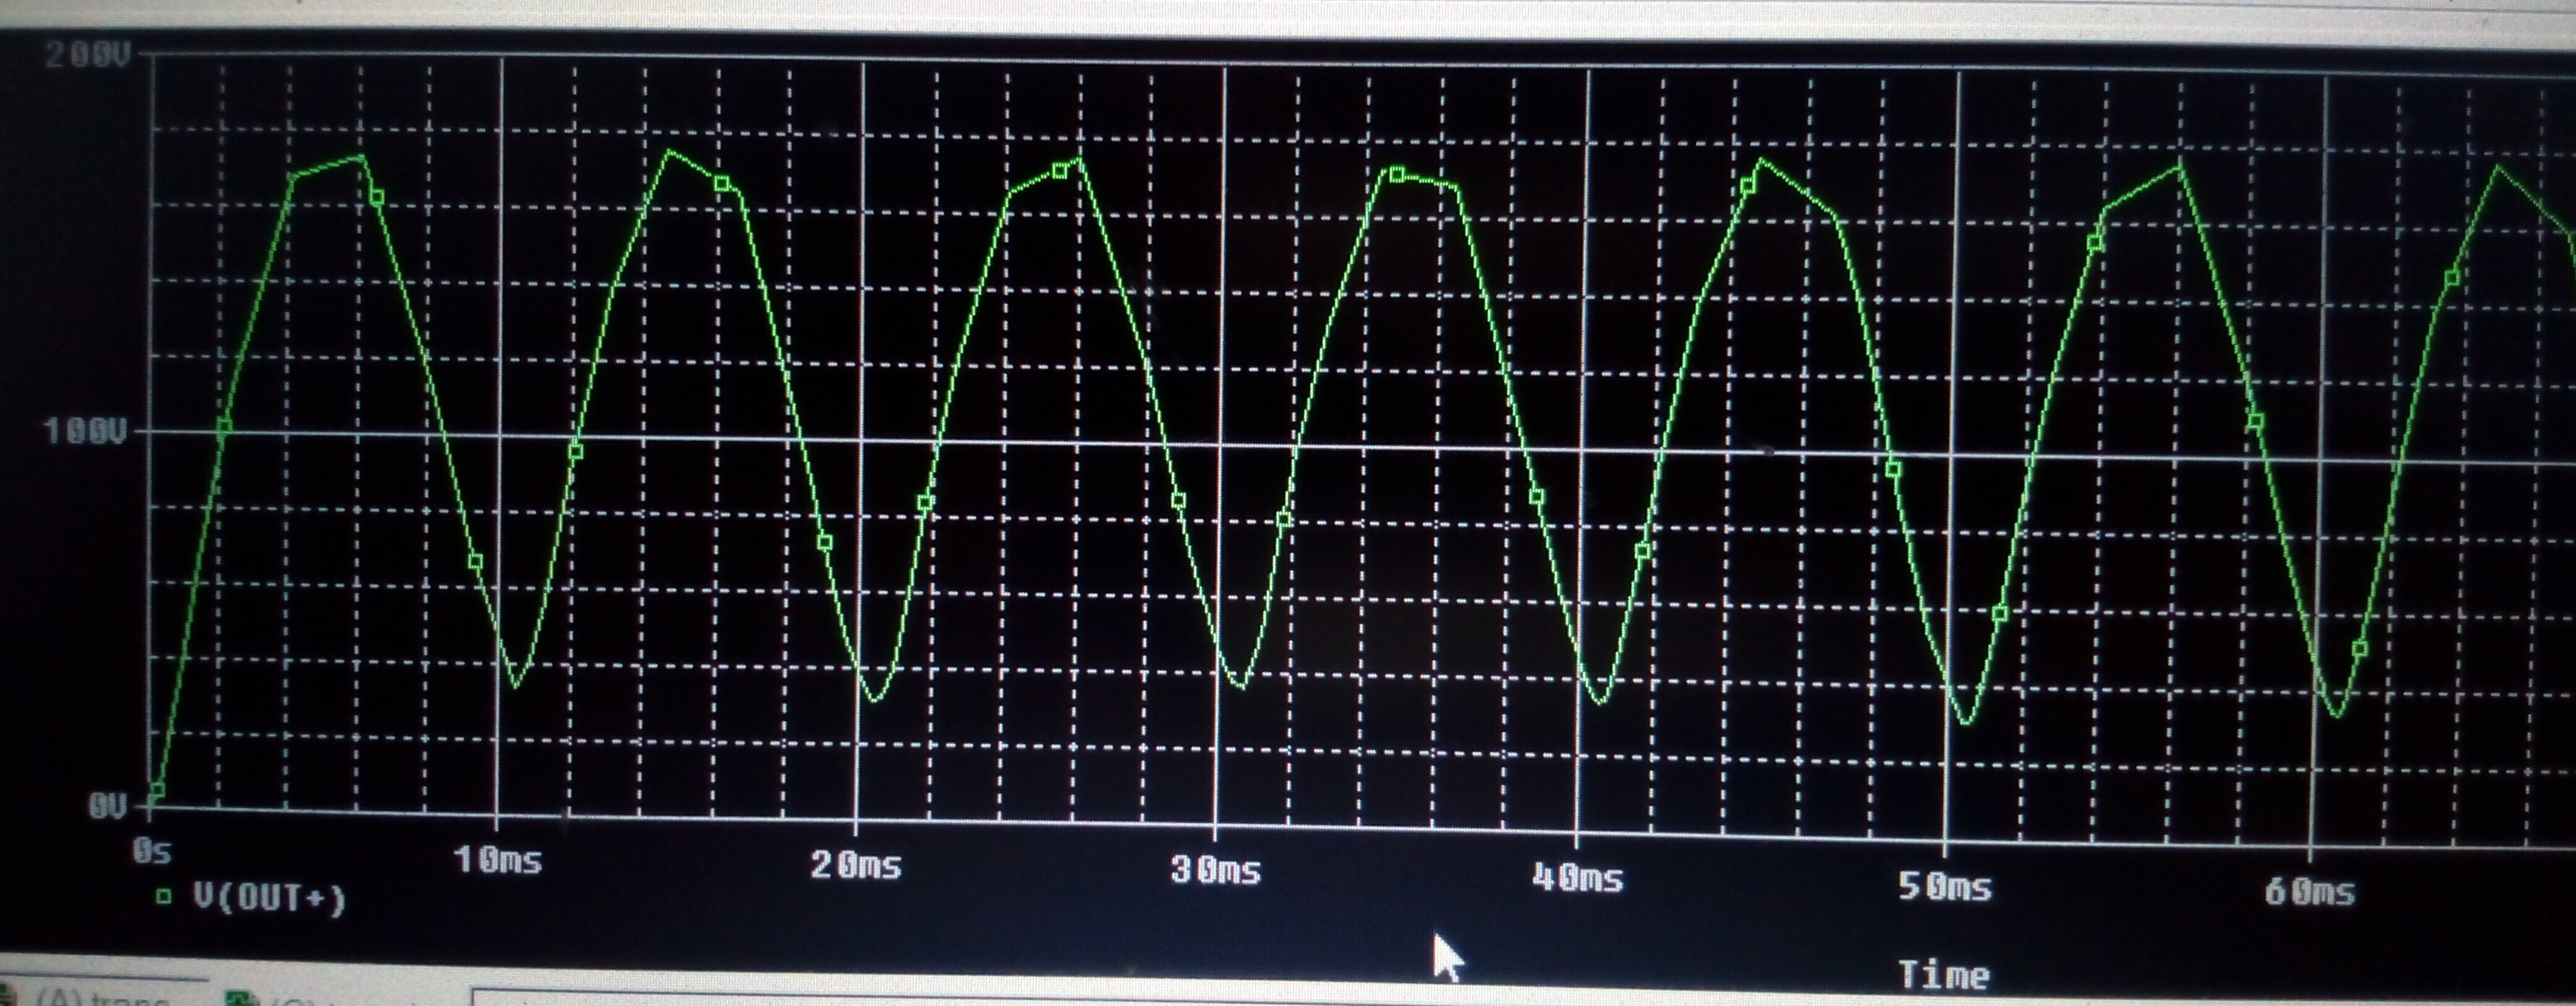
\includegraphics[width=8cm]{Escritorio/Practica 1/6.jpg}
\caption{V(out) en una R=1,rectificador monofasico en fuente}
\end{figure}


\begin{figure}[hbtp]
\centering
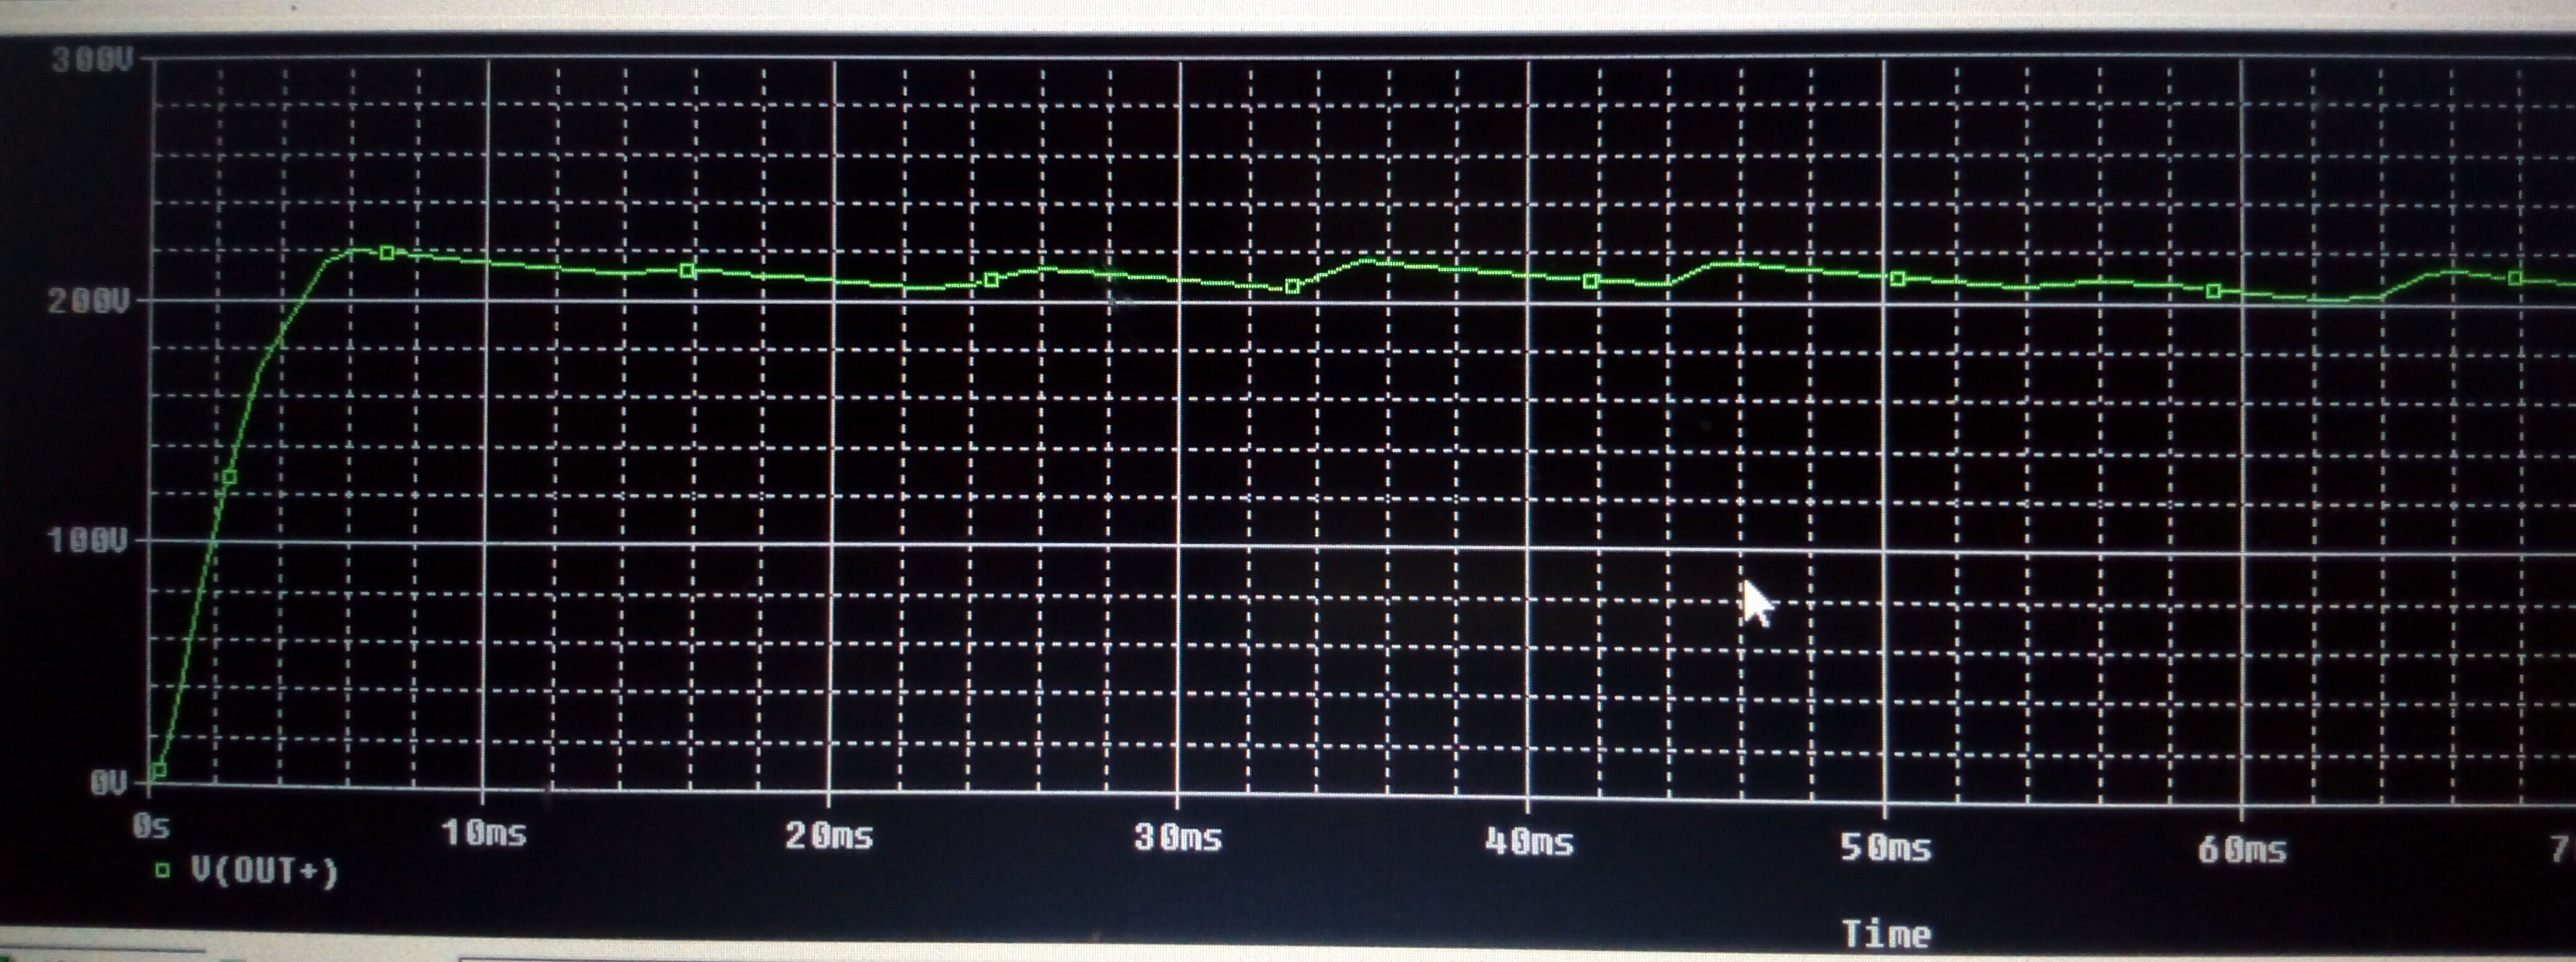
\includegraphics[width=8cm]{Escritorio/Practica 1/7.jpg}
\caption{V(out, rectificador monofasico en fuente), R=100}
\end{figure}


\begin{figure}[hbtp]
\centering
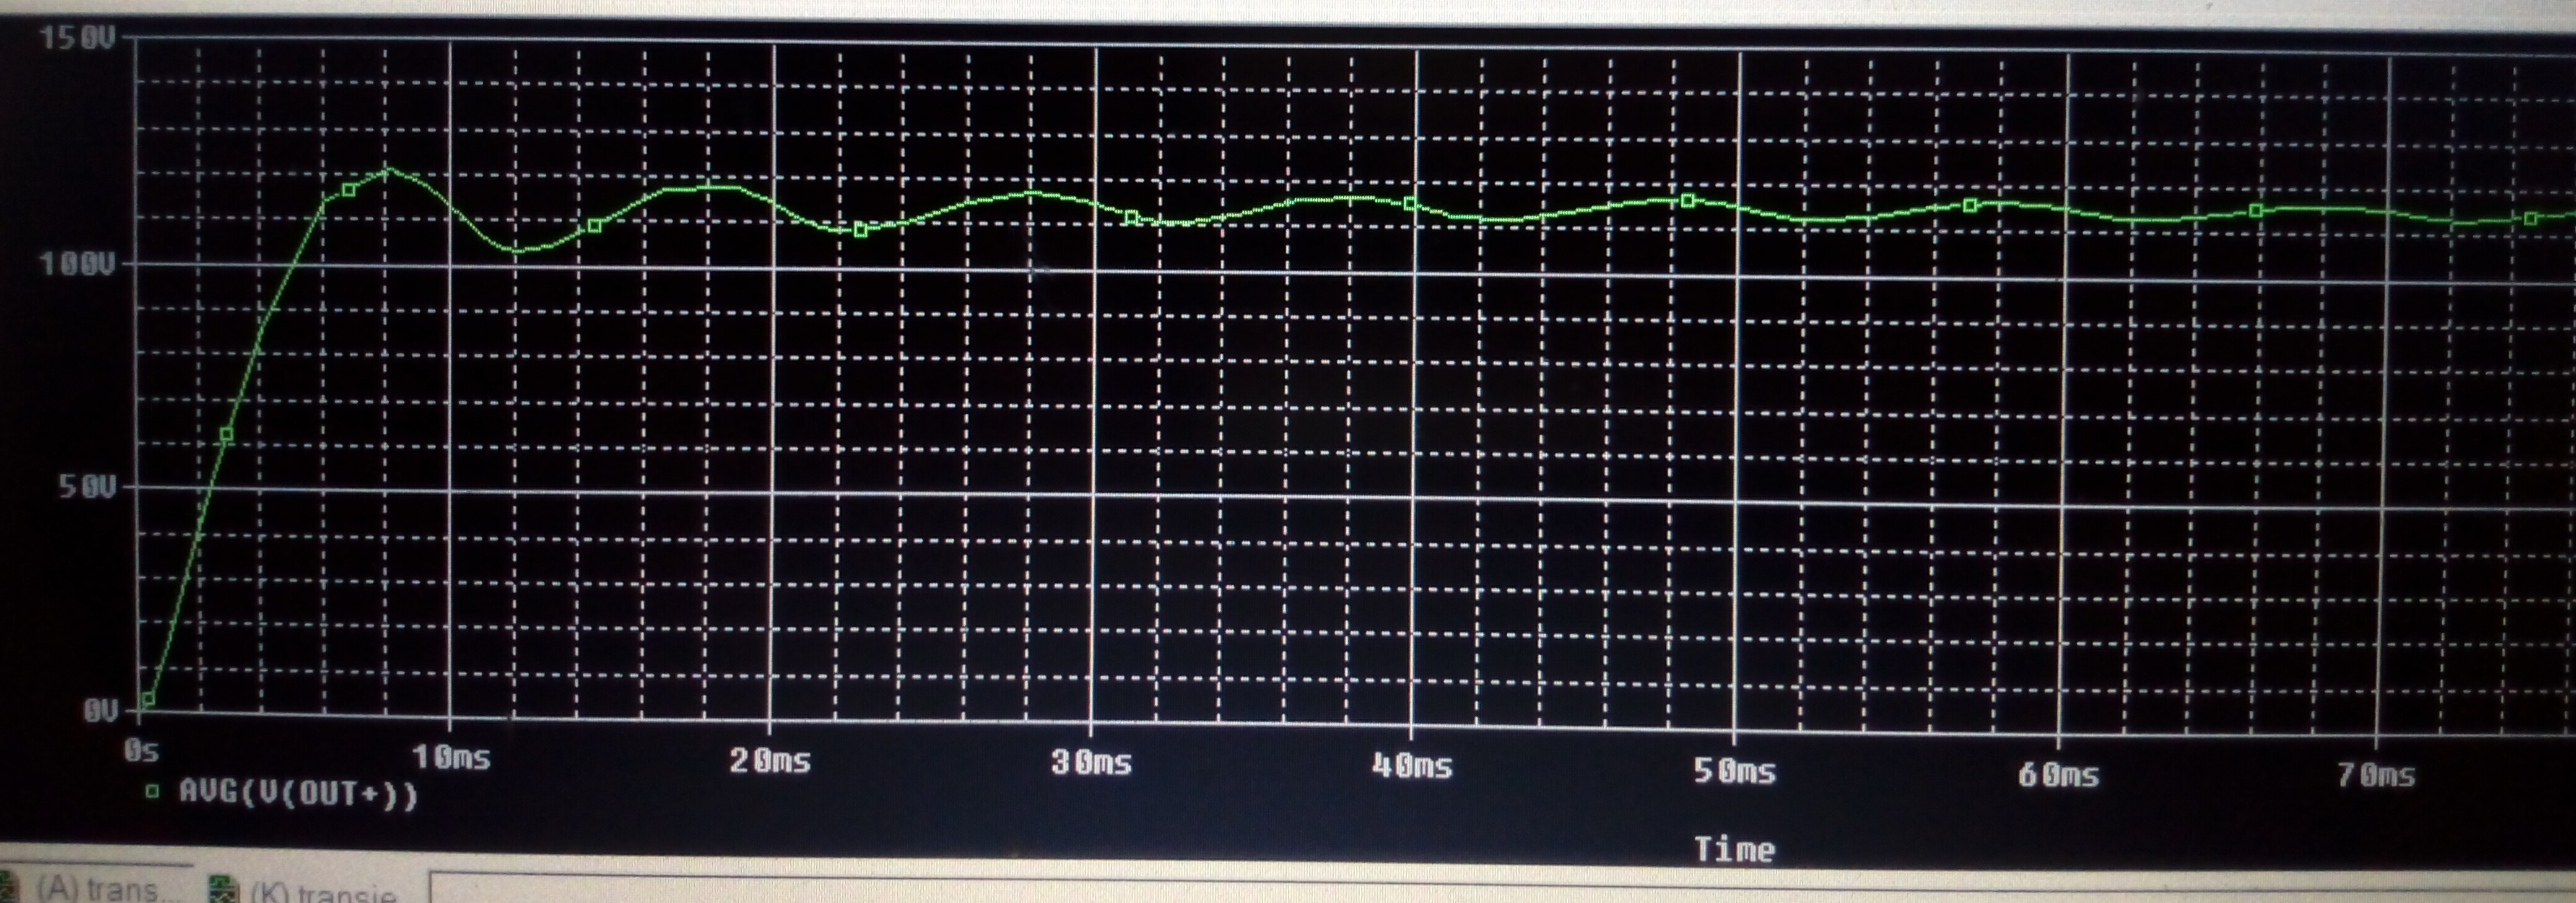
\includegraphics[width=8cm]{Escritorio/Practica 1/9.jpg}
\caption{AVG(Vout), R=1, rectificador monofasico en fuente}
\end{figure}

\begin{figure}[hbtp]
\centering
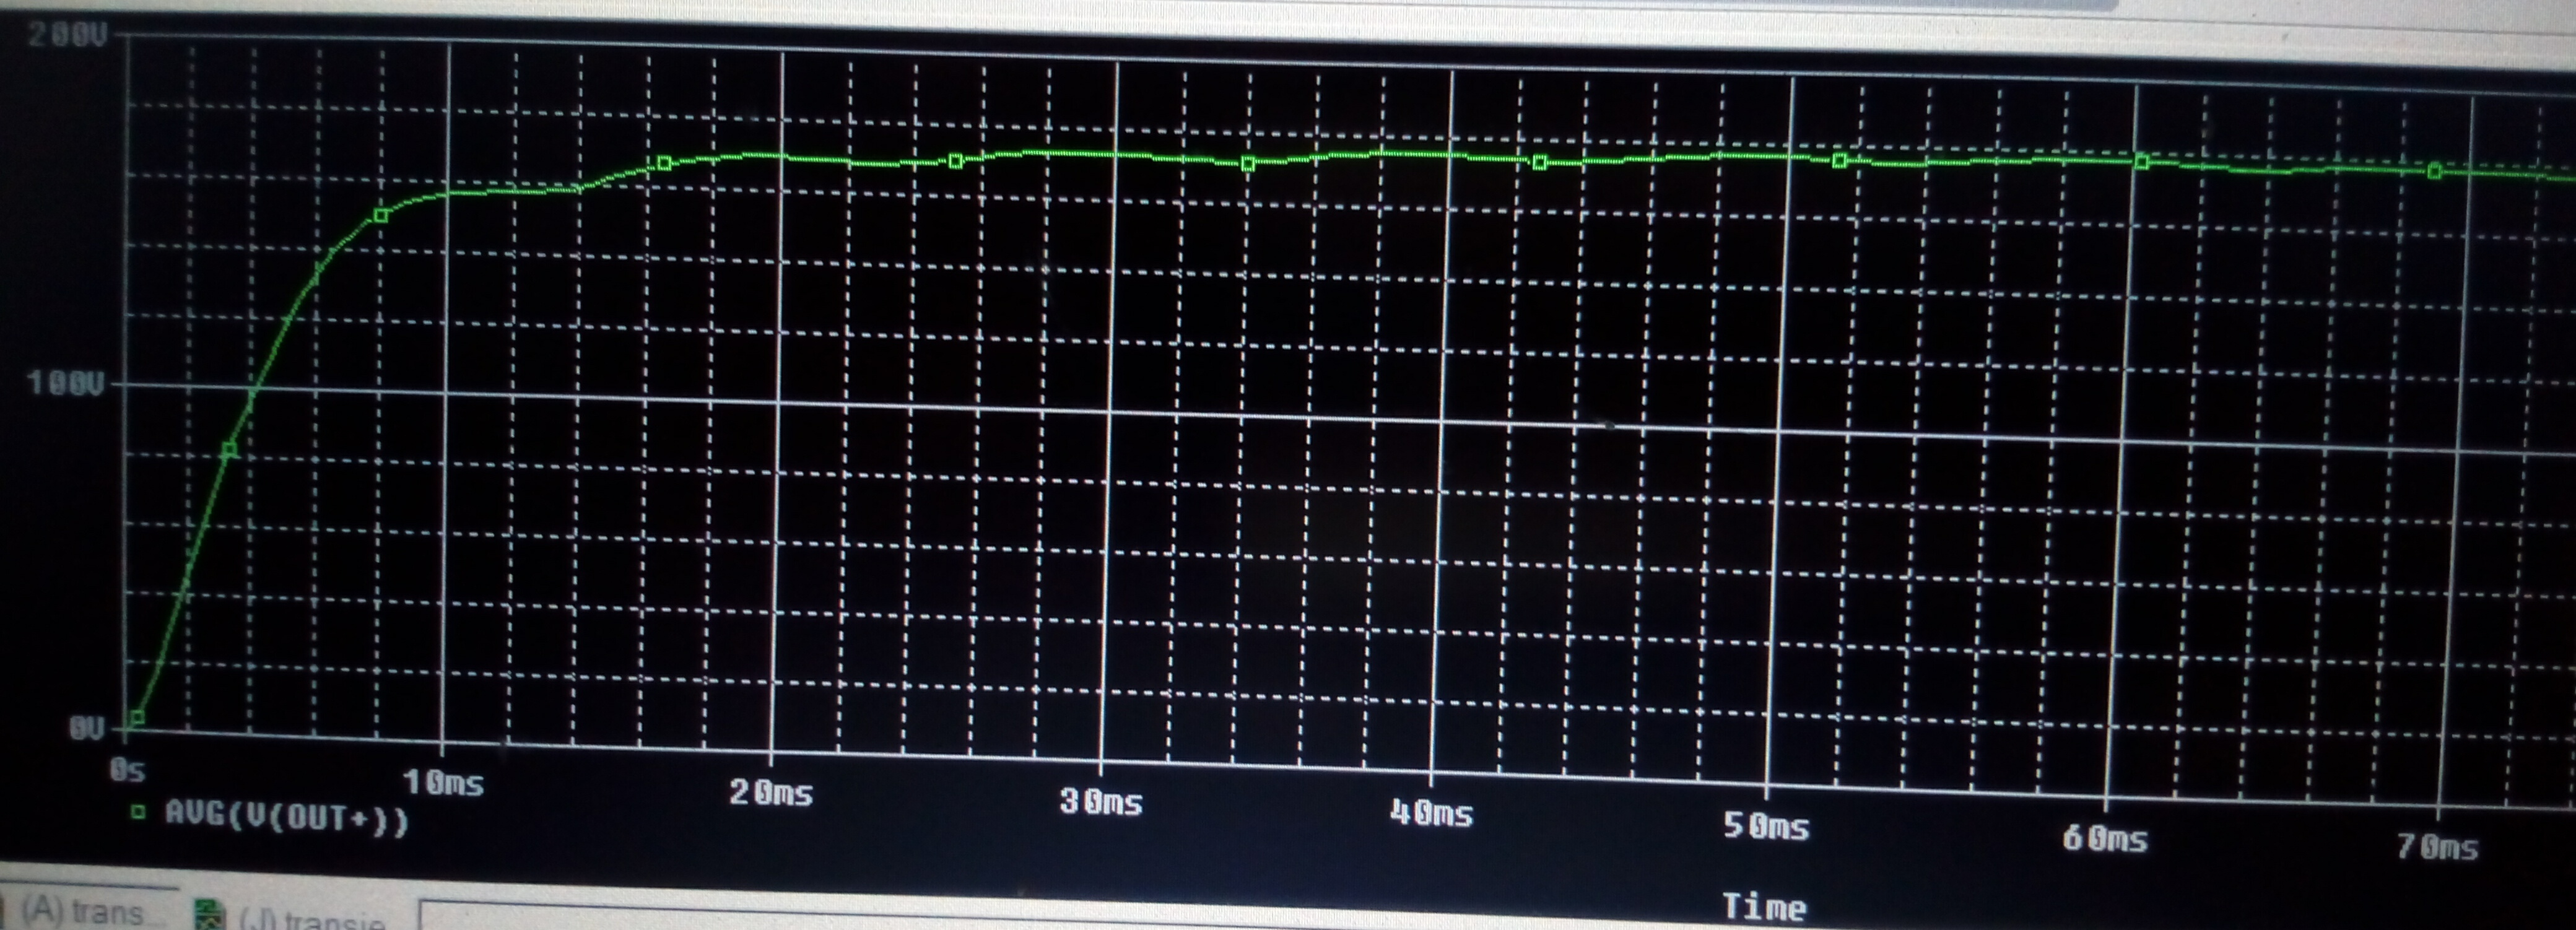
\includegraphics[width=8cm]{Escritorio/Practica 1/8.jpg}
\caption{AVG(Vout), R=10, rectificador monofasico en fuente}
\end{figure}


\begin{figure}[hbtp]
\centering
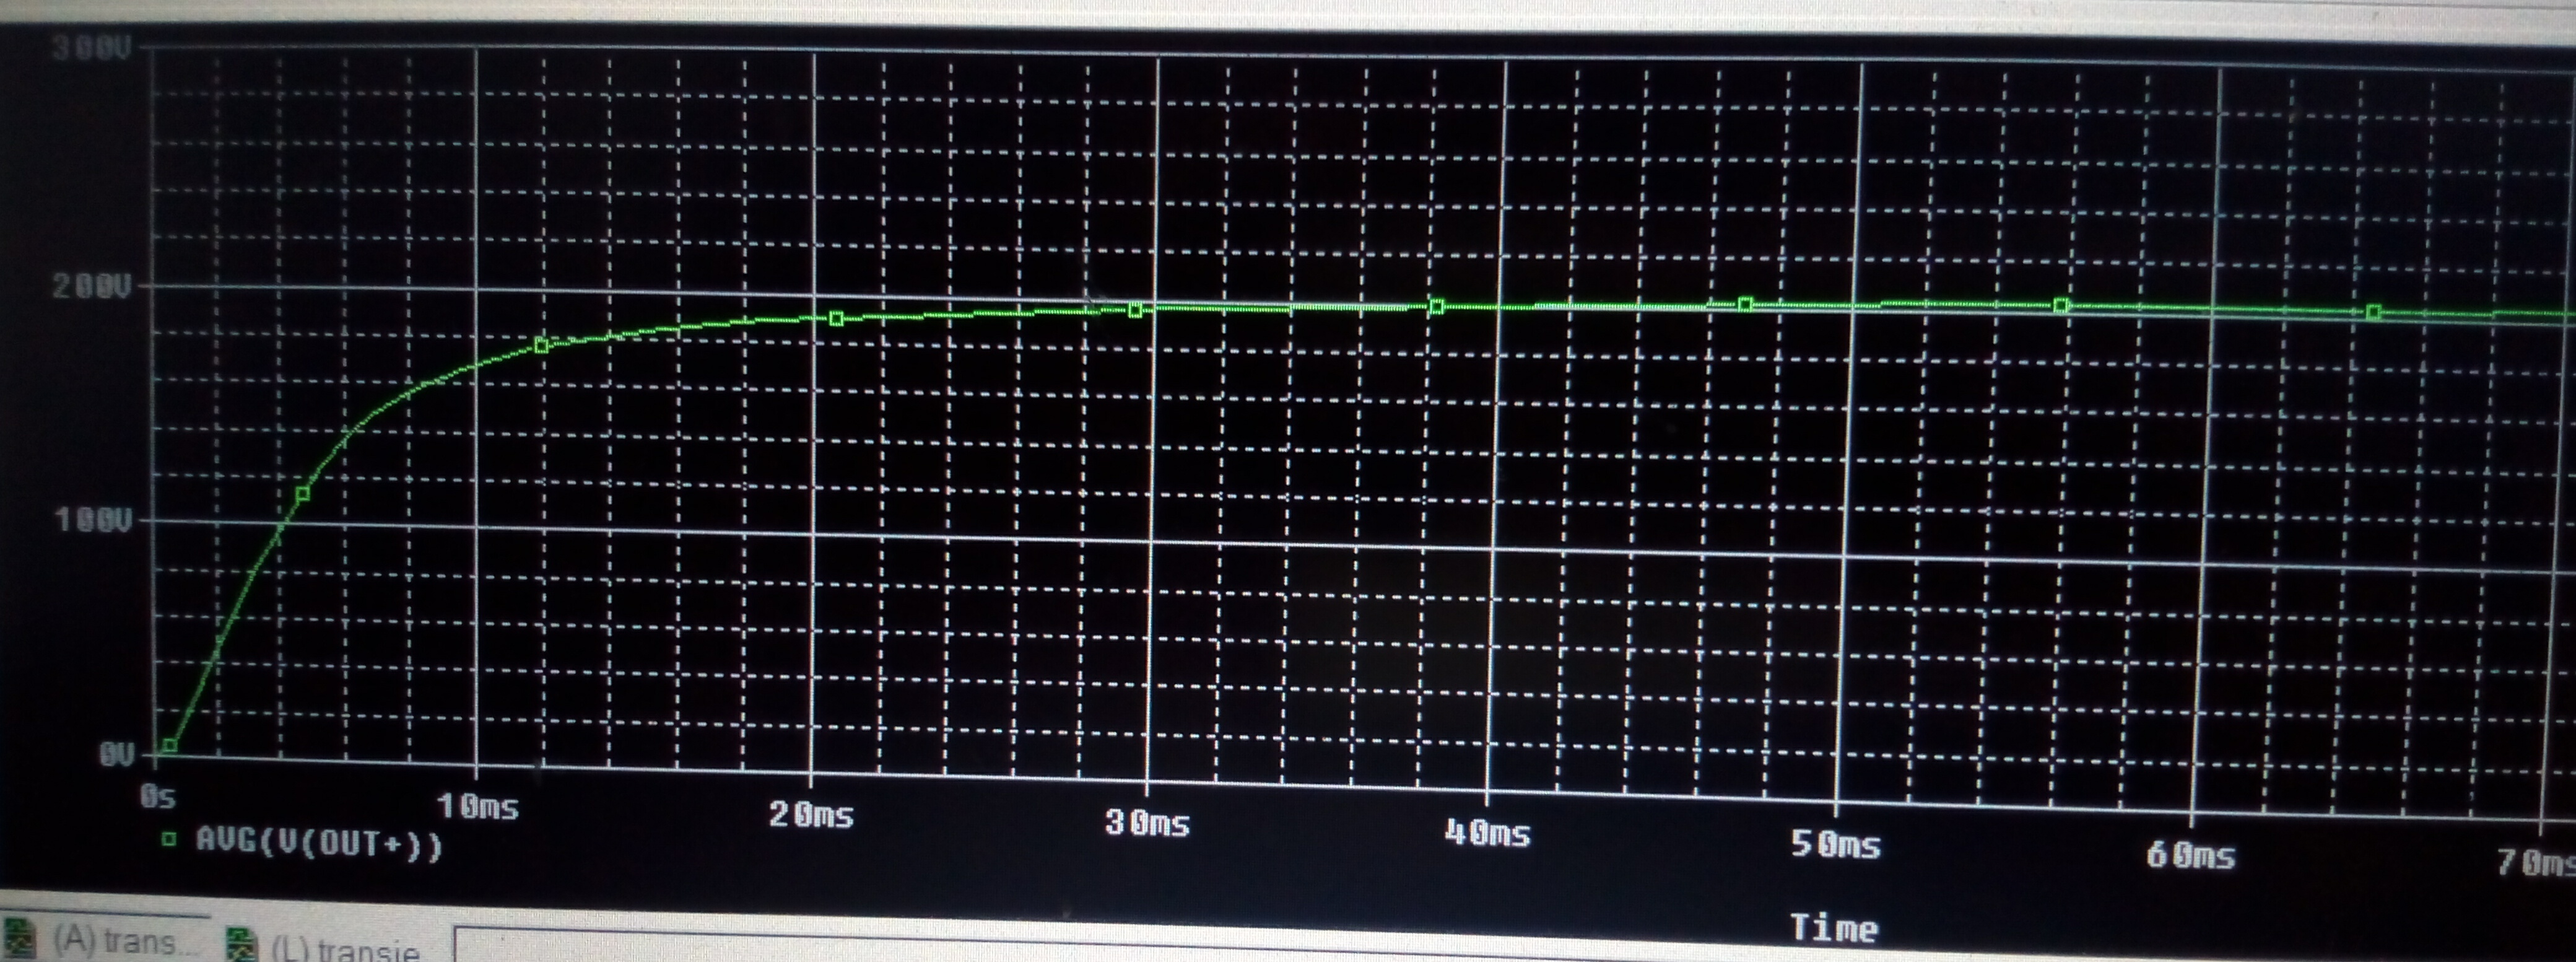
\includegraphics[width=8cm]{Escritorio/Practica 1/10.jpg}
\caption{AVG(Vout), R=100, rectificador monofasico en fuente}
\end{figure}

\begin{figure}[hbtp]
\centering
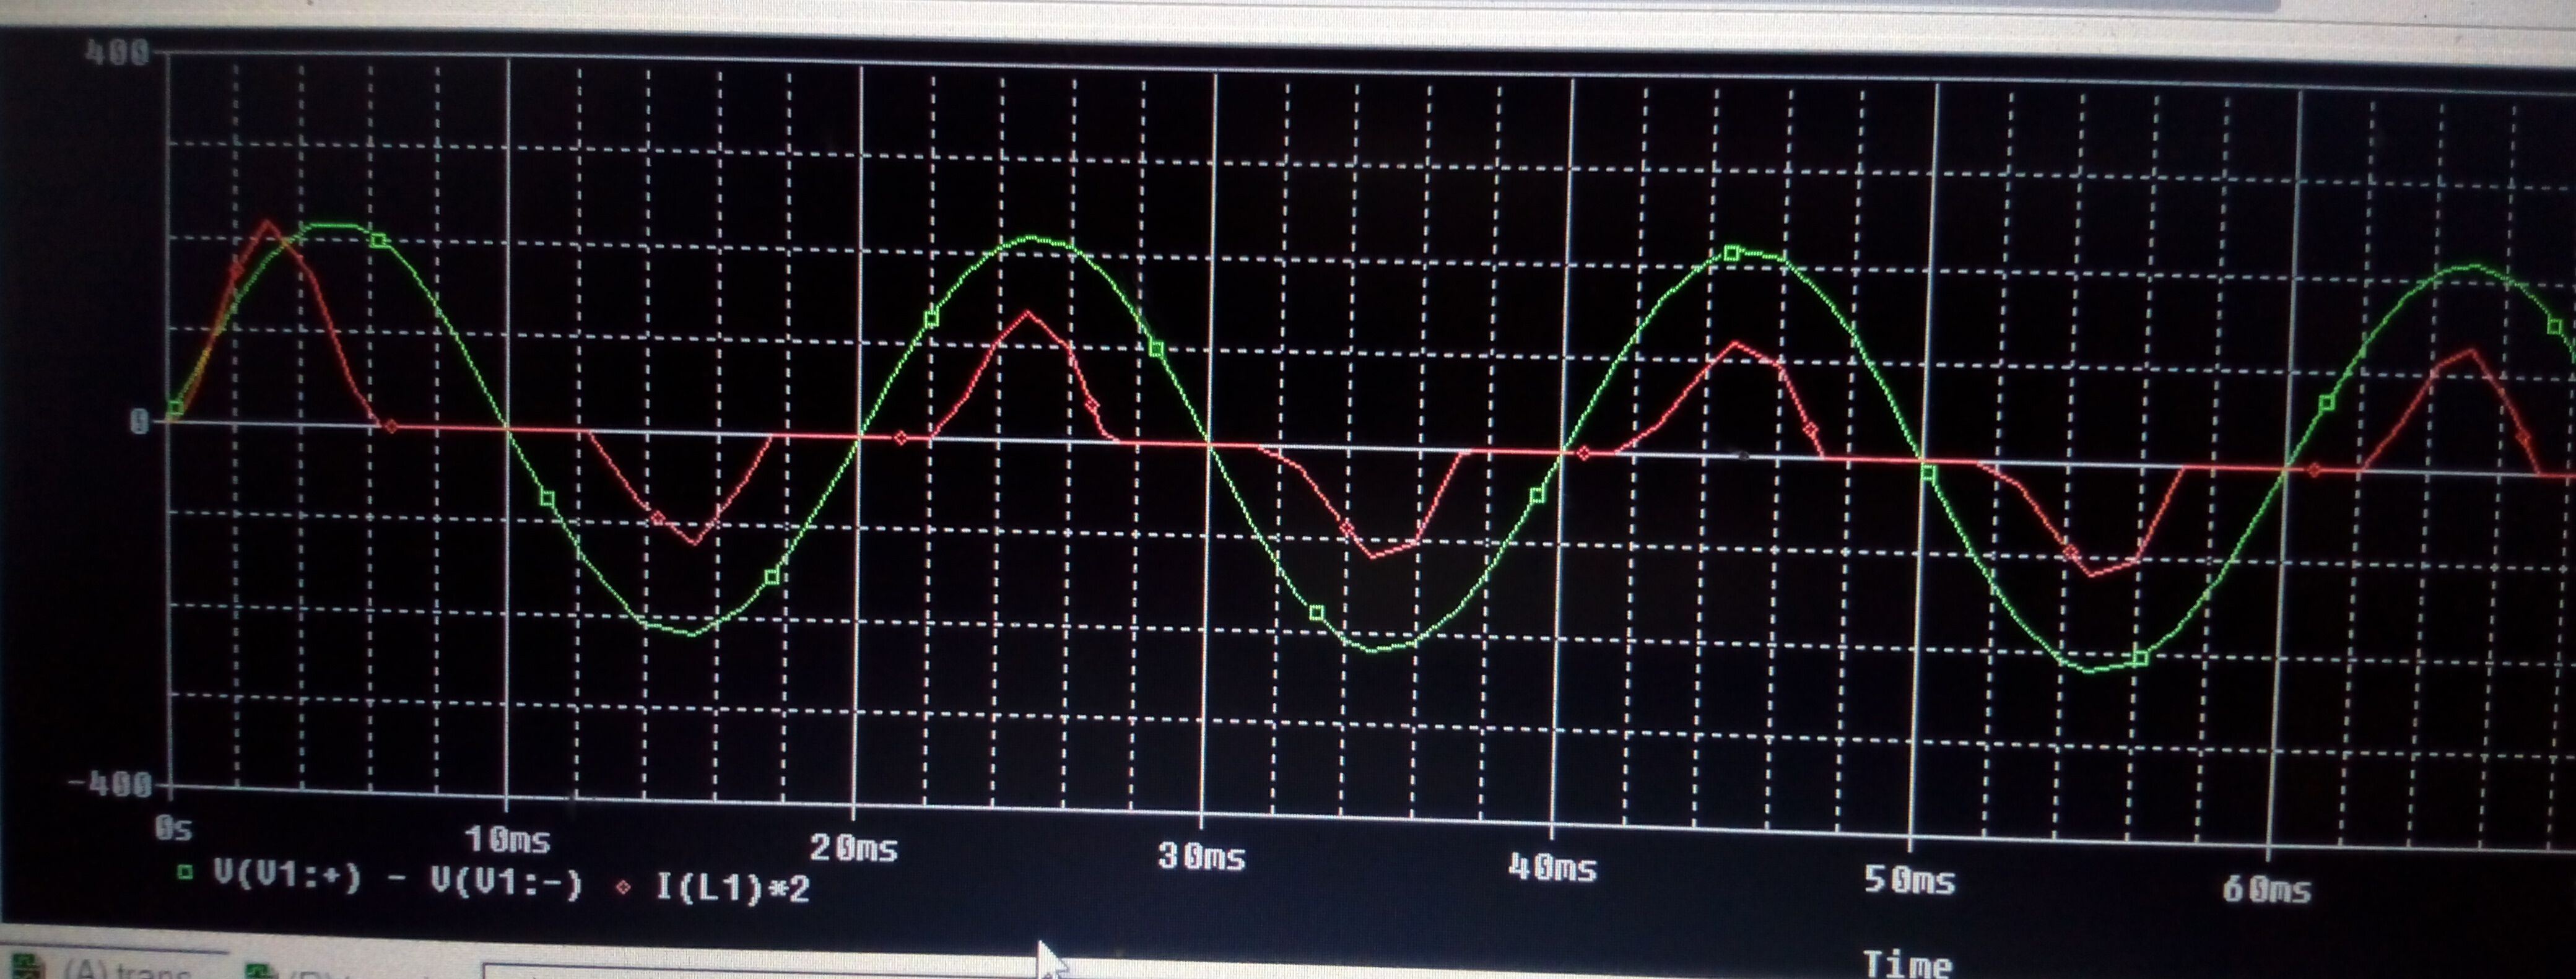
\includegraphics[width=8cm]{Escritorio/Practica 1/11.jpg}
\caption{V(V1:+)-V(V1:-), I(L1), rectificador monofasico en fuente}
\end{figure}


\begin{figure}[hbtp]
\centering
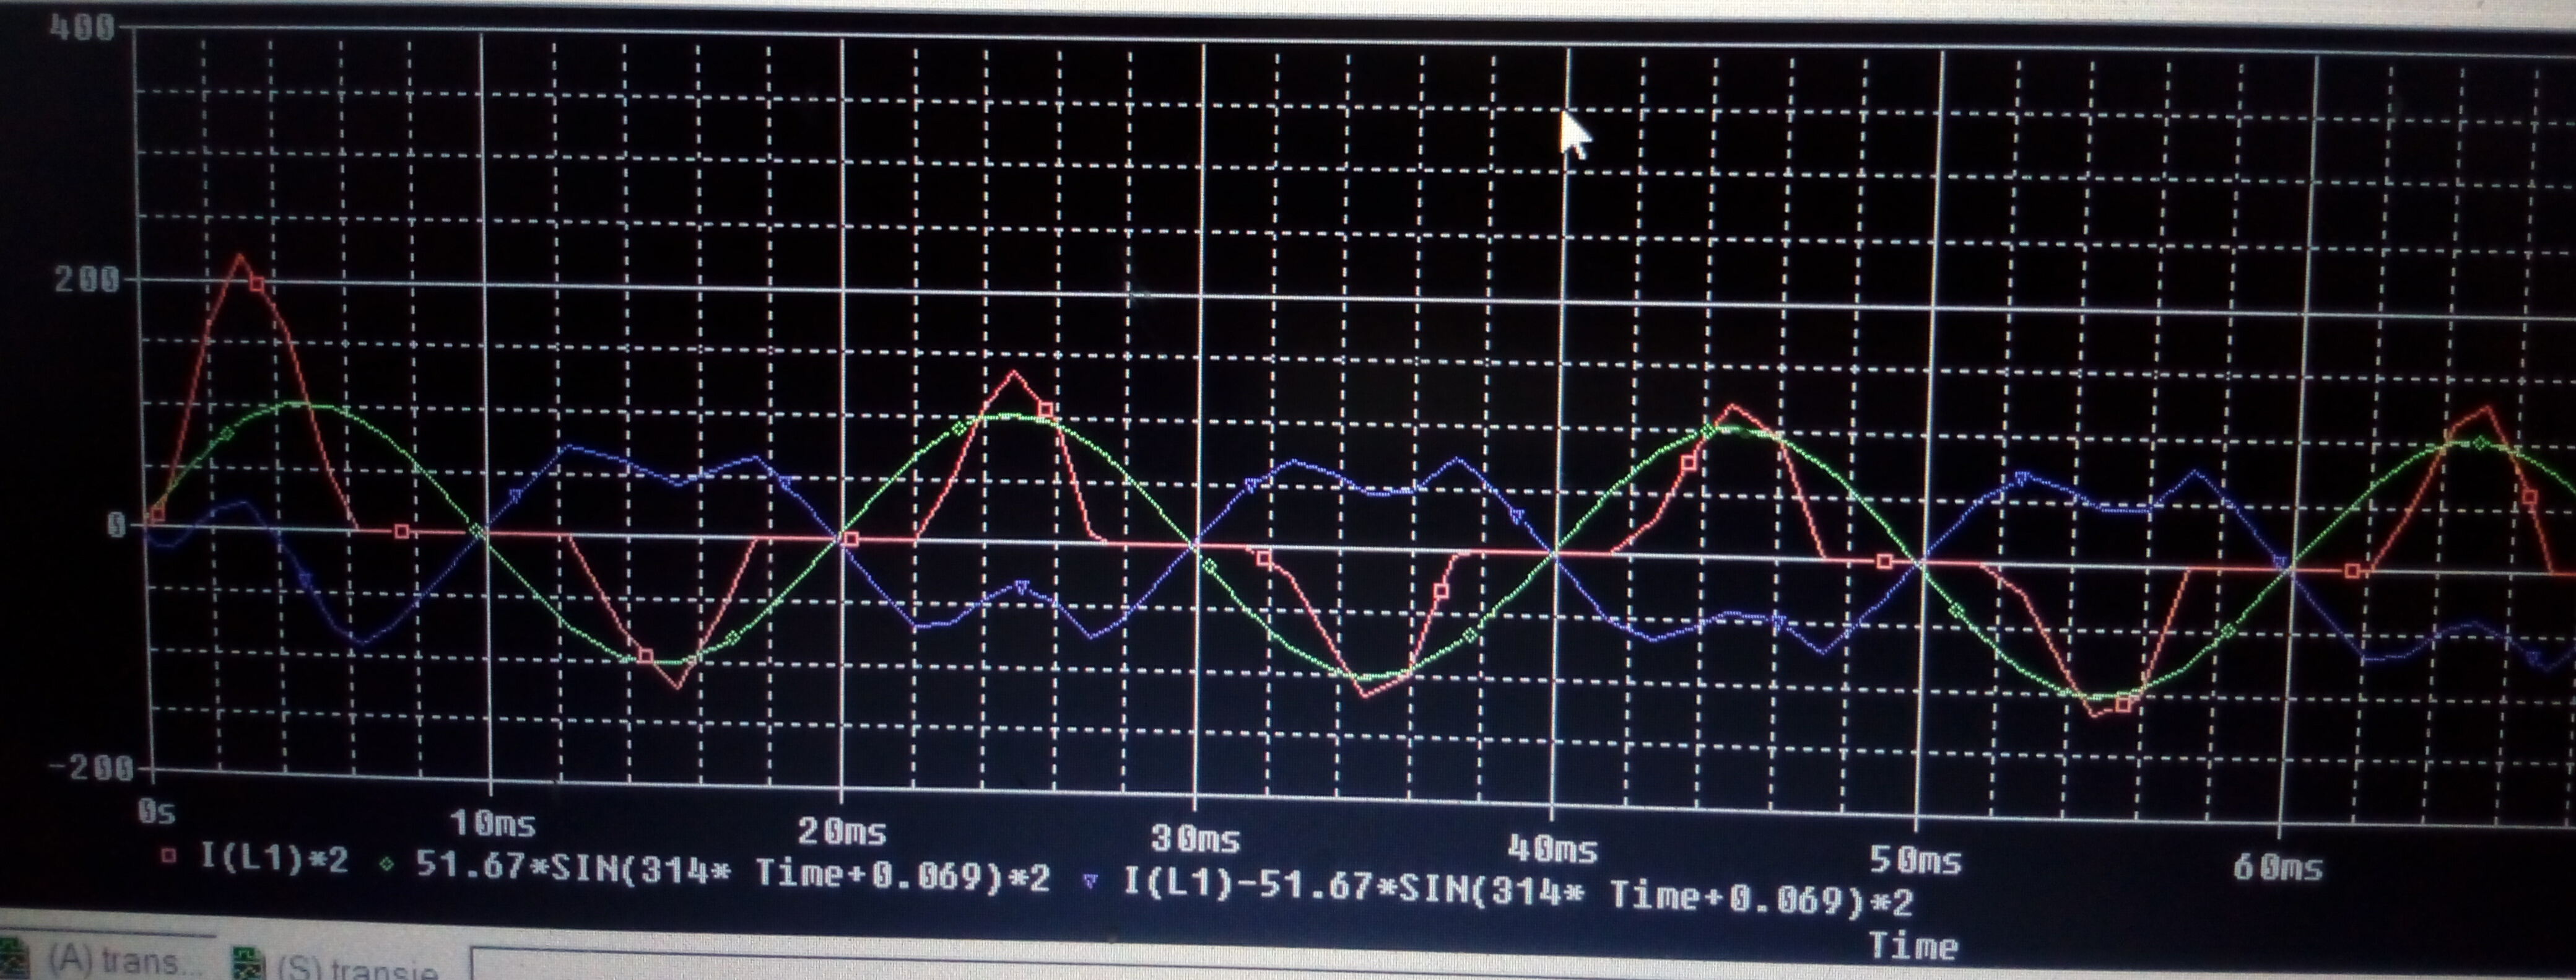
\includegraphics[width=8cm]{Escritorio/Practica 1/12.jpg}
\caption{I(L1)-51.67*sin(314*time+0.069), rectificador monofasico en fuente}
\end{figure}


\begin{figure}[hbtp]
\centering
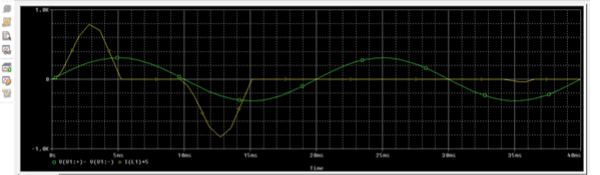
\includegraphics[width=8cm]{Escritorio/Practica 1/31.png}
\caption{V(PCC), I(L1) Estudio de la tension en PCC}
\end{figure}

\begin{figure}[hbtp]
\centering
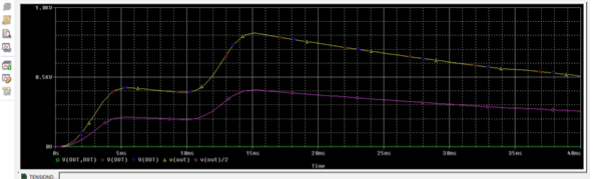
\includegraphics[width=8cm]{Escritorio/Practica 1/33.png}
\caption{V(OUT), Rectificador monofasico duplicador de tension}
\end{figure}

\begin{figure}[hbtp]
\centering
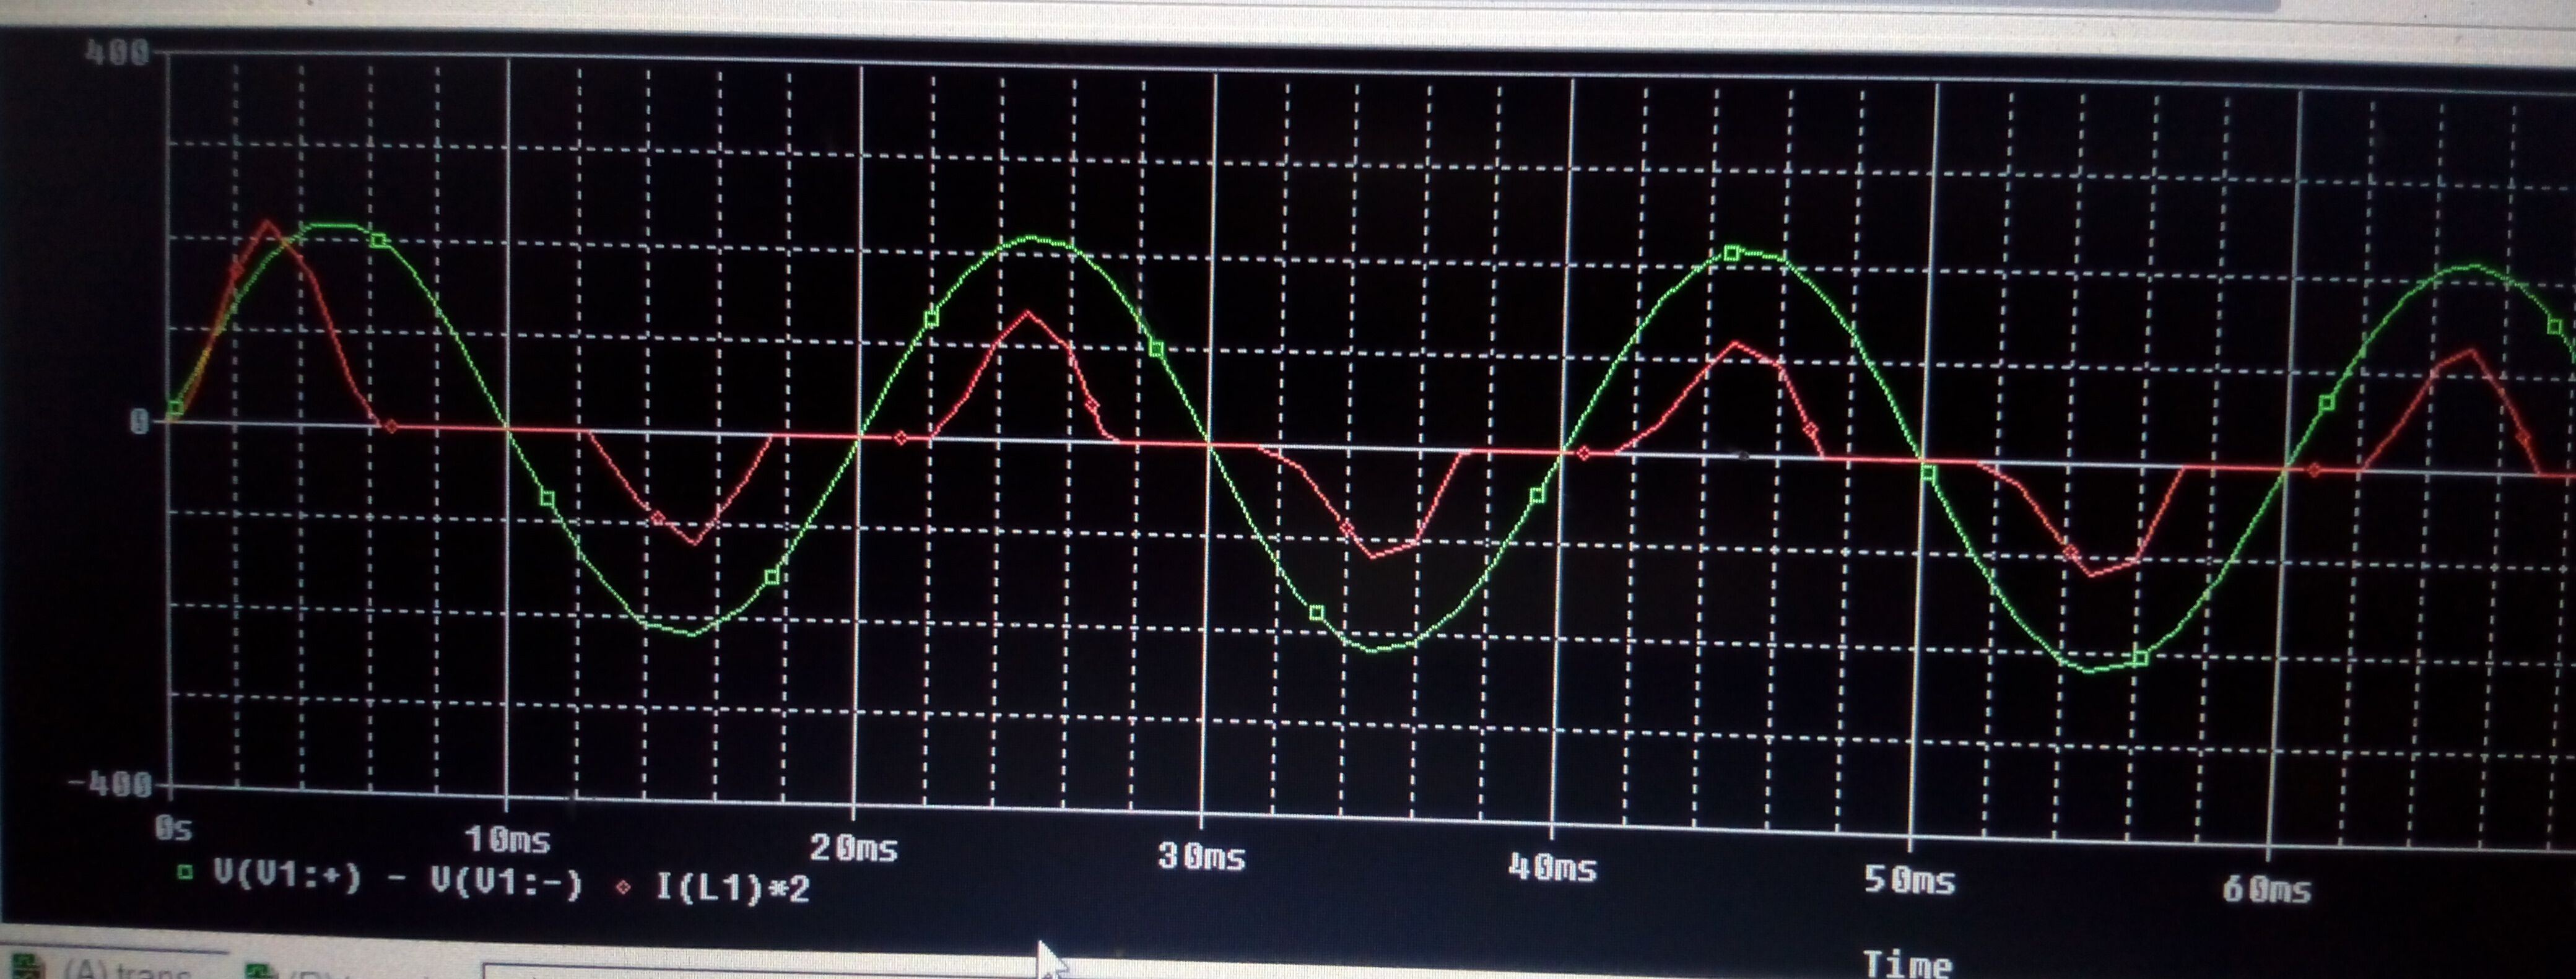
\includegraphics[width=8cm]{Escritorio/Practica 1/35.jpg}
\caption{V(out), I(L1)  Rectificador monofasico duplicador de tension}
\end{figure}

\begin{figure}[hbtp]
\centering
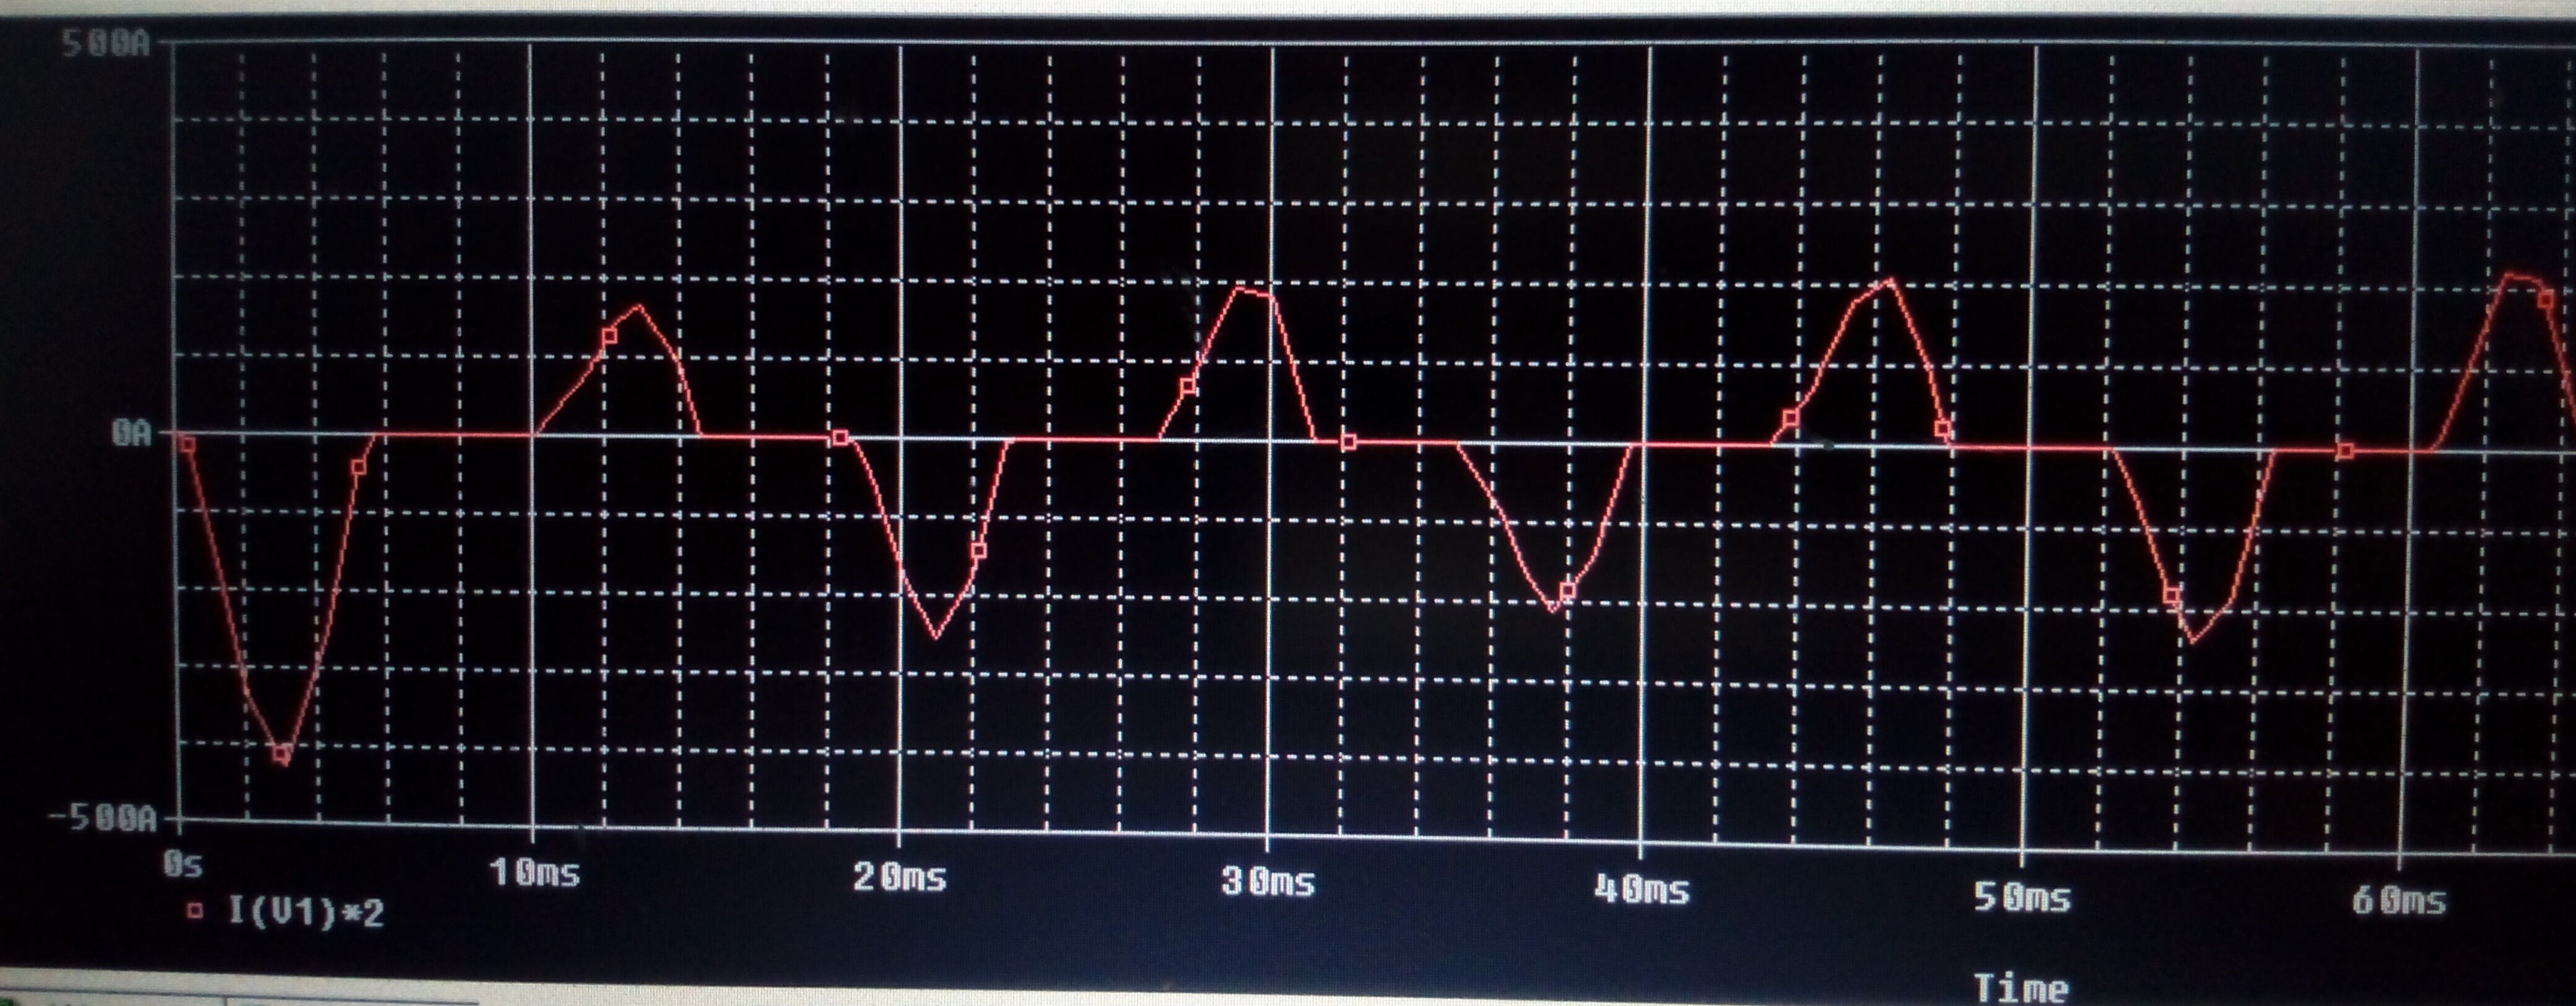
\includegraphics[width=8cm]{Escritorio/Practica 1/13.jpg}
\caption{I(V1), Rectificador monofasico en lineas trifasicas}
\end{figure}


\begin{figure}[hbtp]
\centering
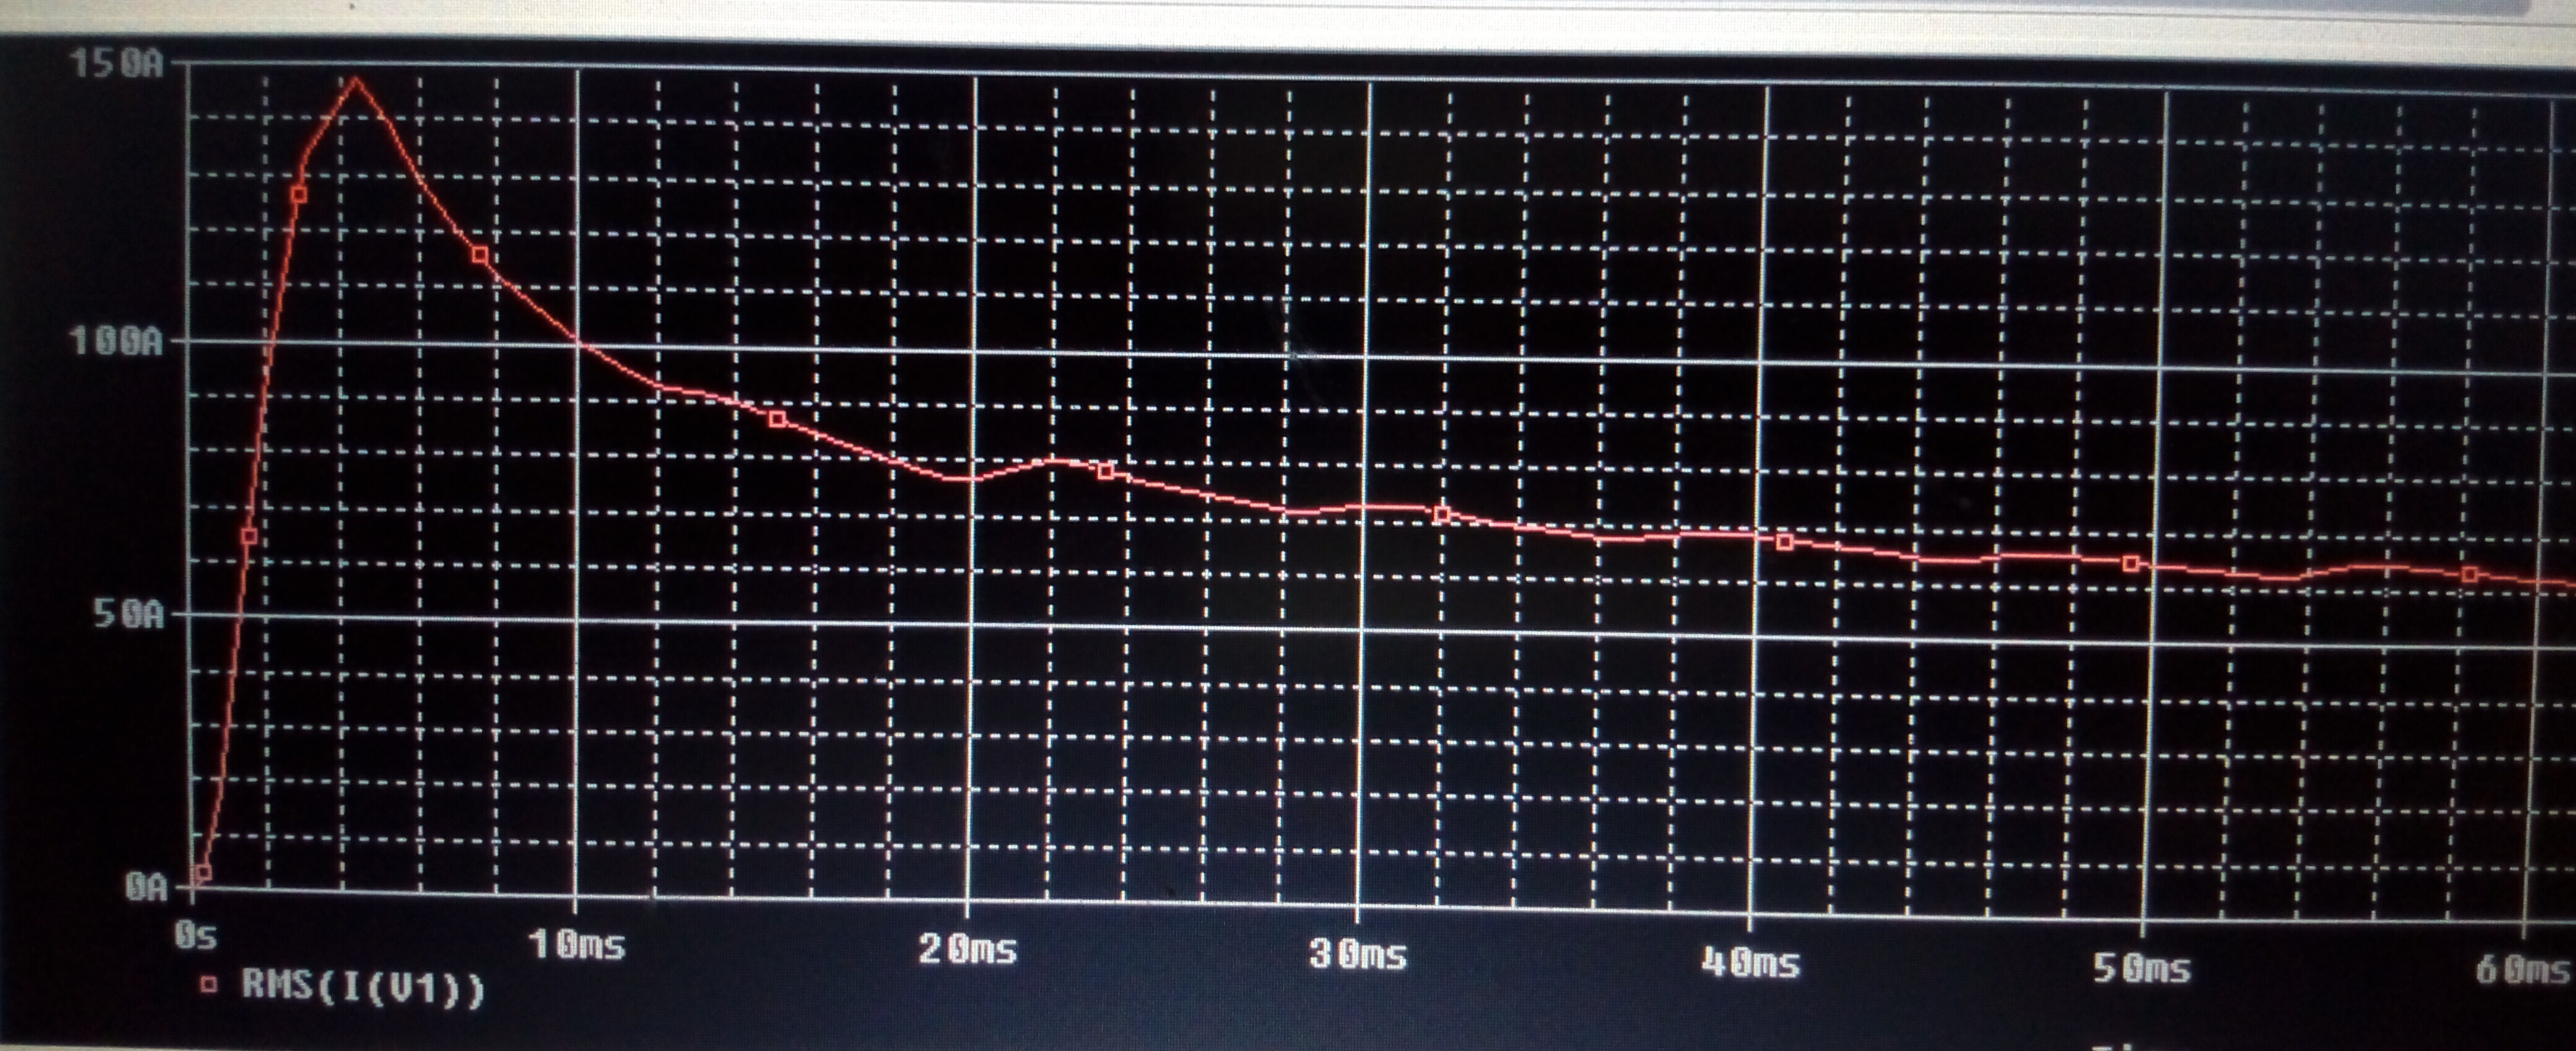
\includegraphics[width=8cm]{Escritorio/Practica 1/14.jpg}
\caption{RMS(I(V1)), Rectificador monofasico en lineas trifasicas}
\end{figure}


\begin{figure}[hbtp]
\centering
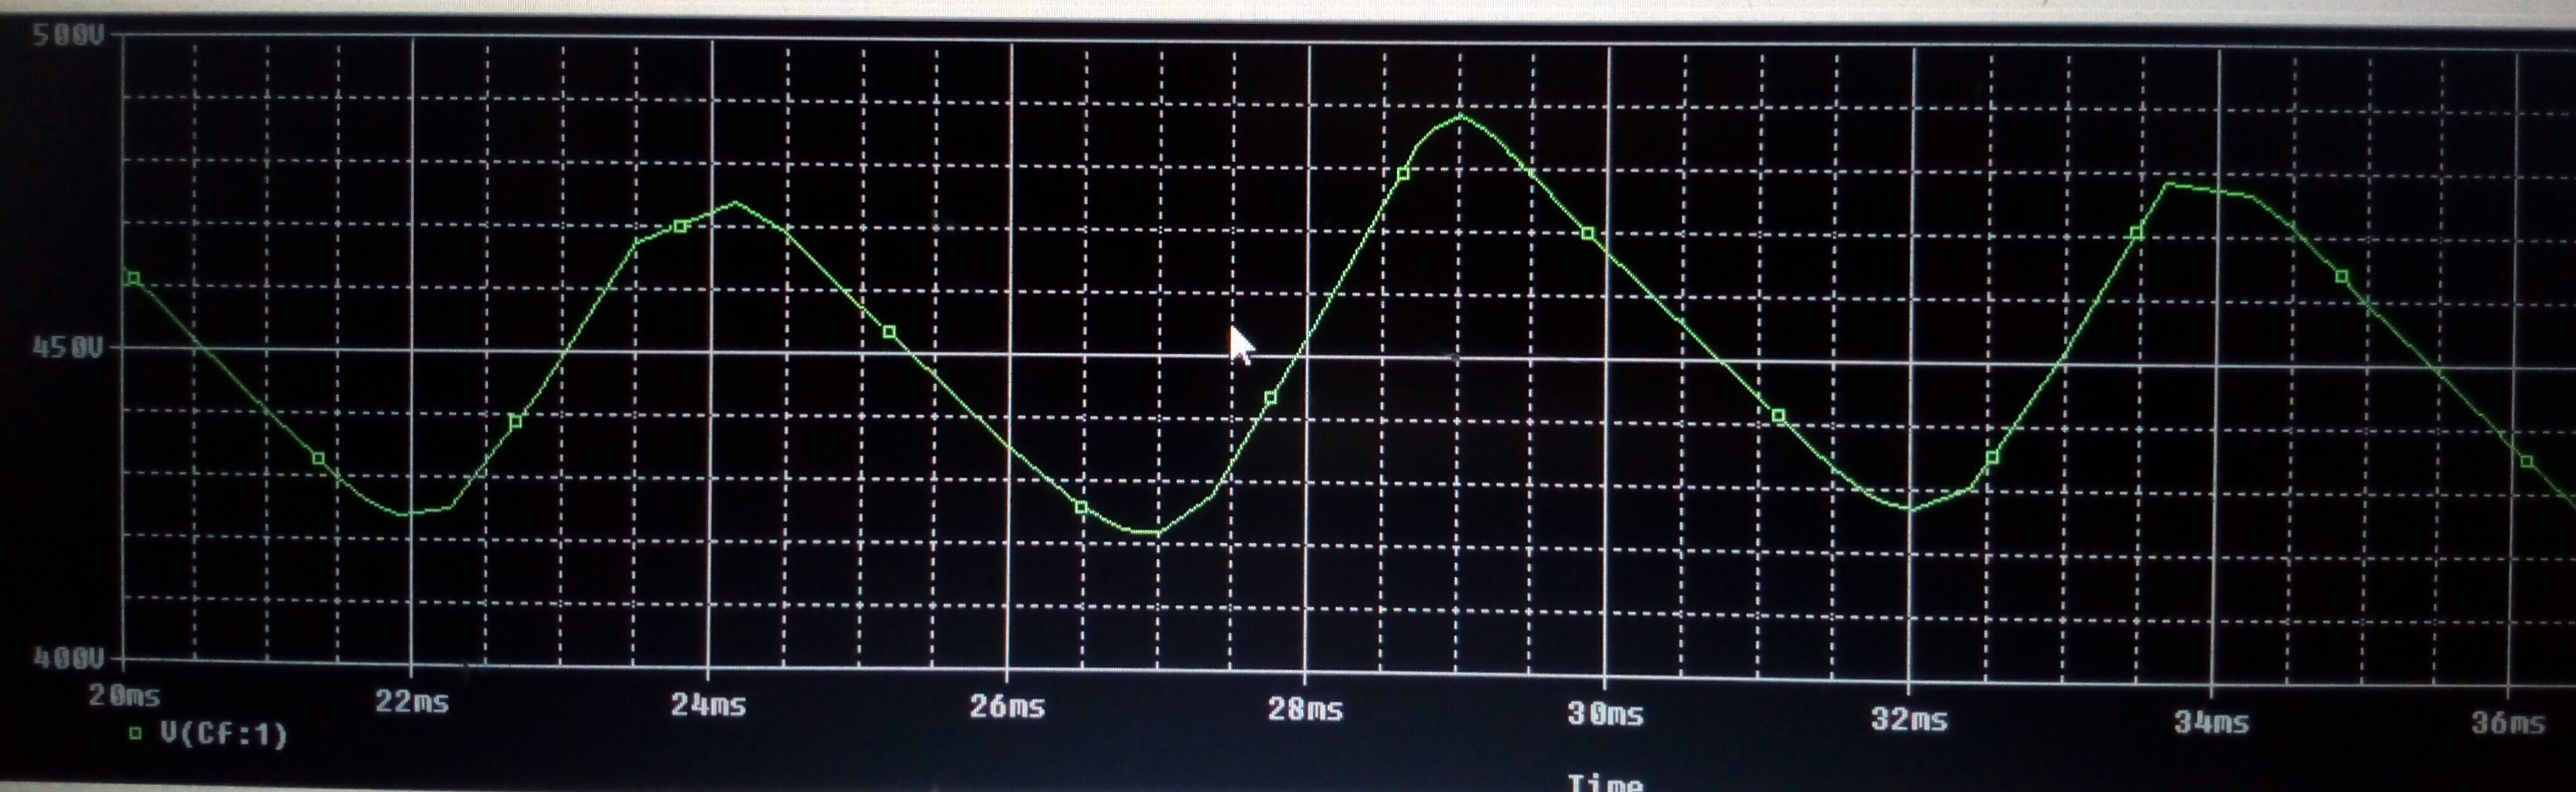
\includegraphics[width=8cm]{Escritorio/Practica 1/17.jpg}
\caption{V(Cf), Rectificador trifasico}
\end{figure}

\begin{figure}[hbtp]
\centering
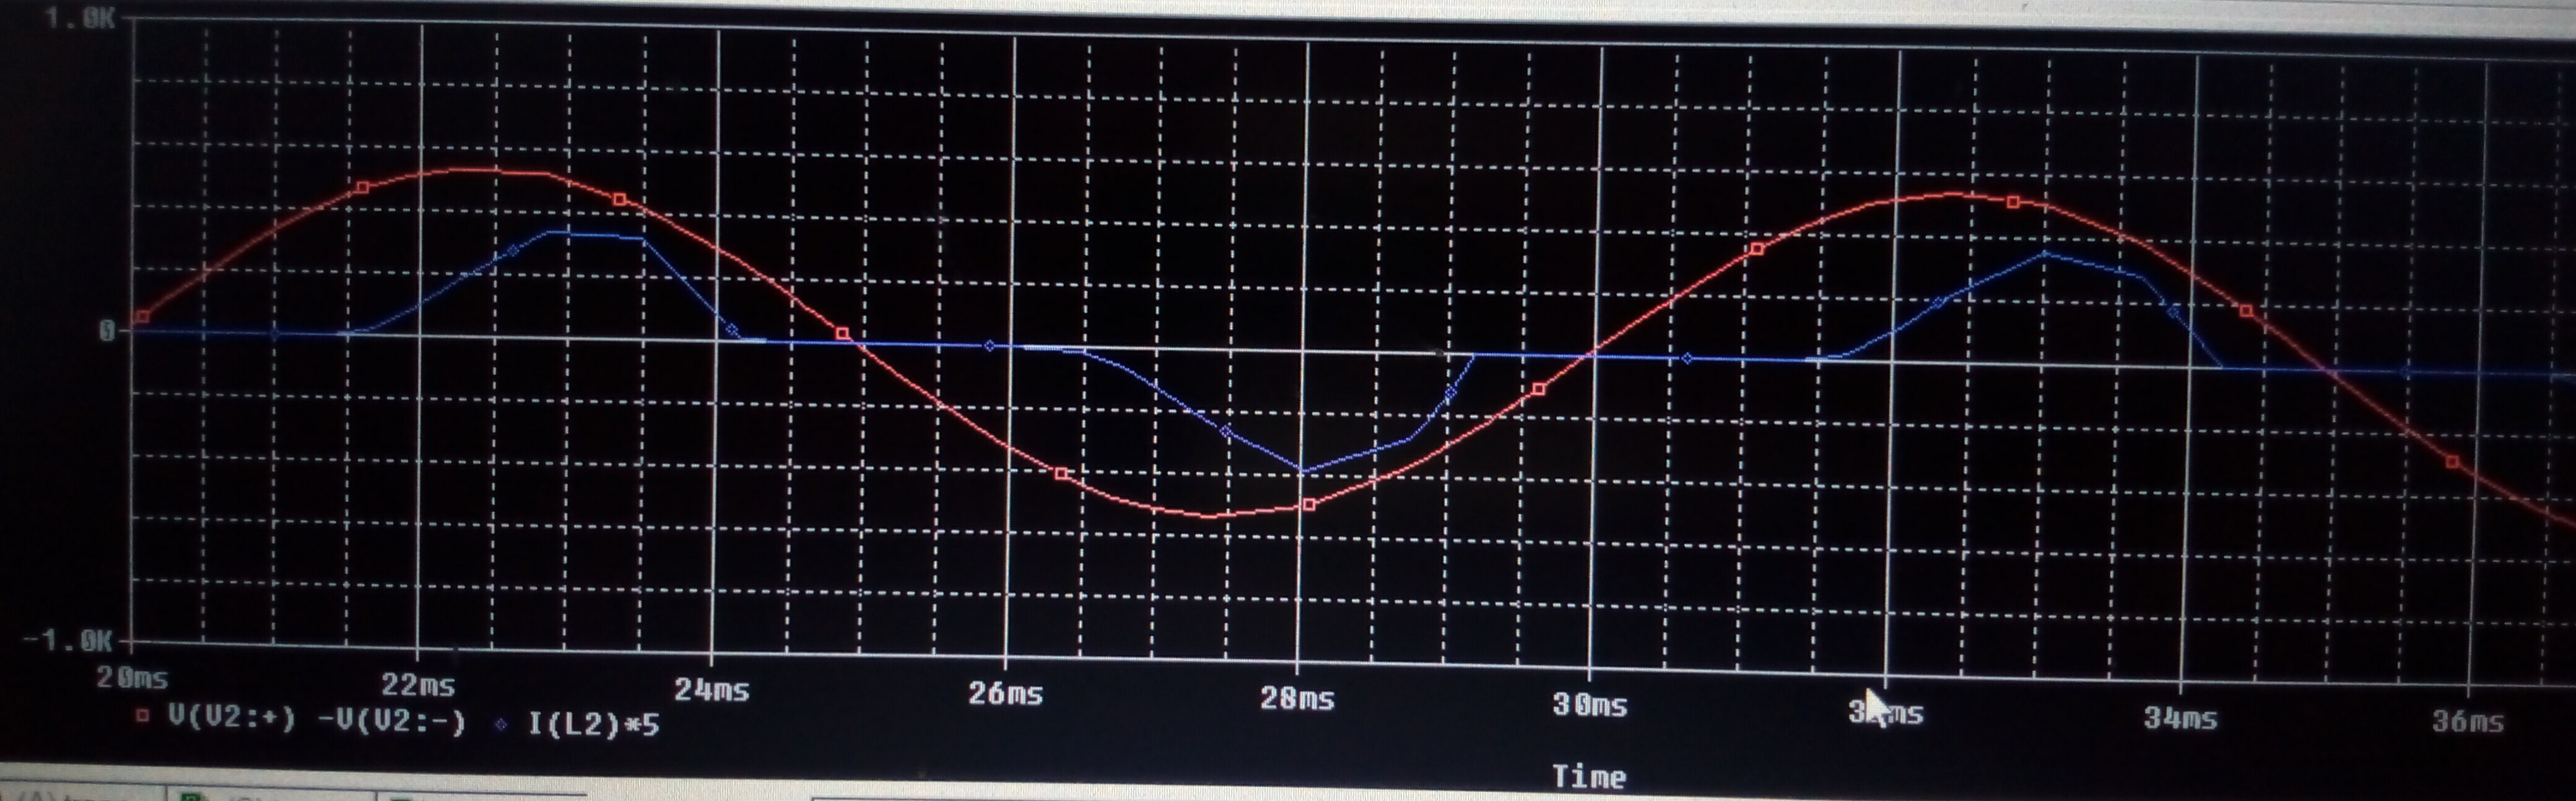
\includegraphics[]{Escritorio/Practica 1/18.jpg}
\caption{V(VL1), (I(L1)*2, tension simple de red de corriente de entrada al rectificador}
\end{figure}


\begin{figure}[hbtp]
\centering
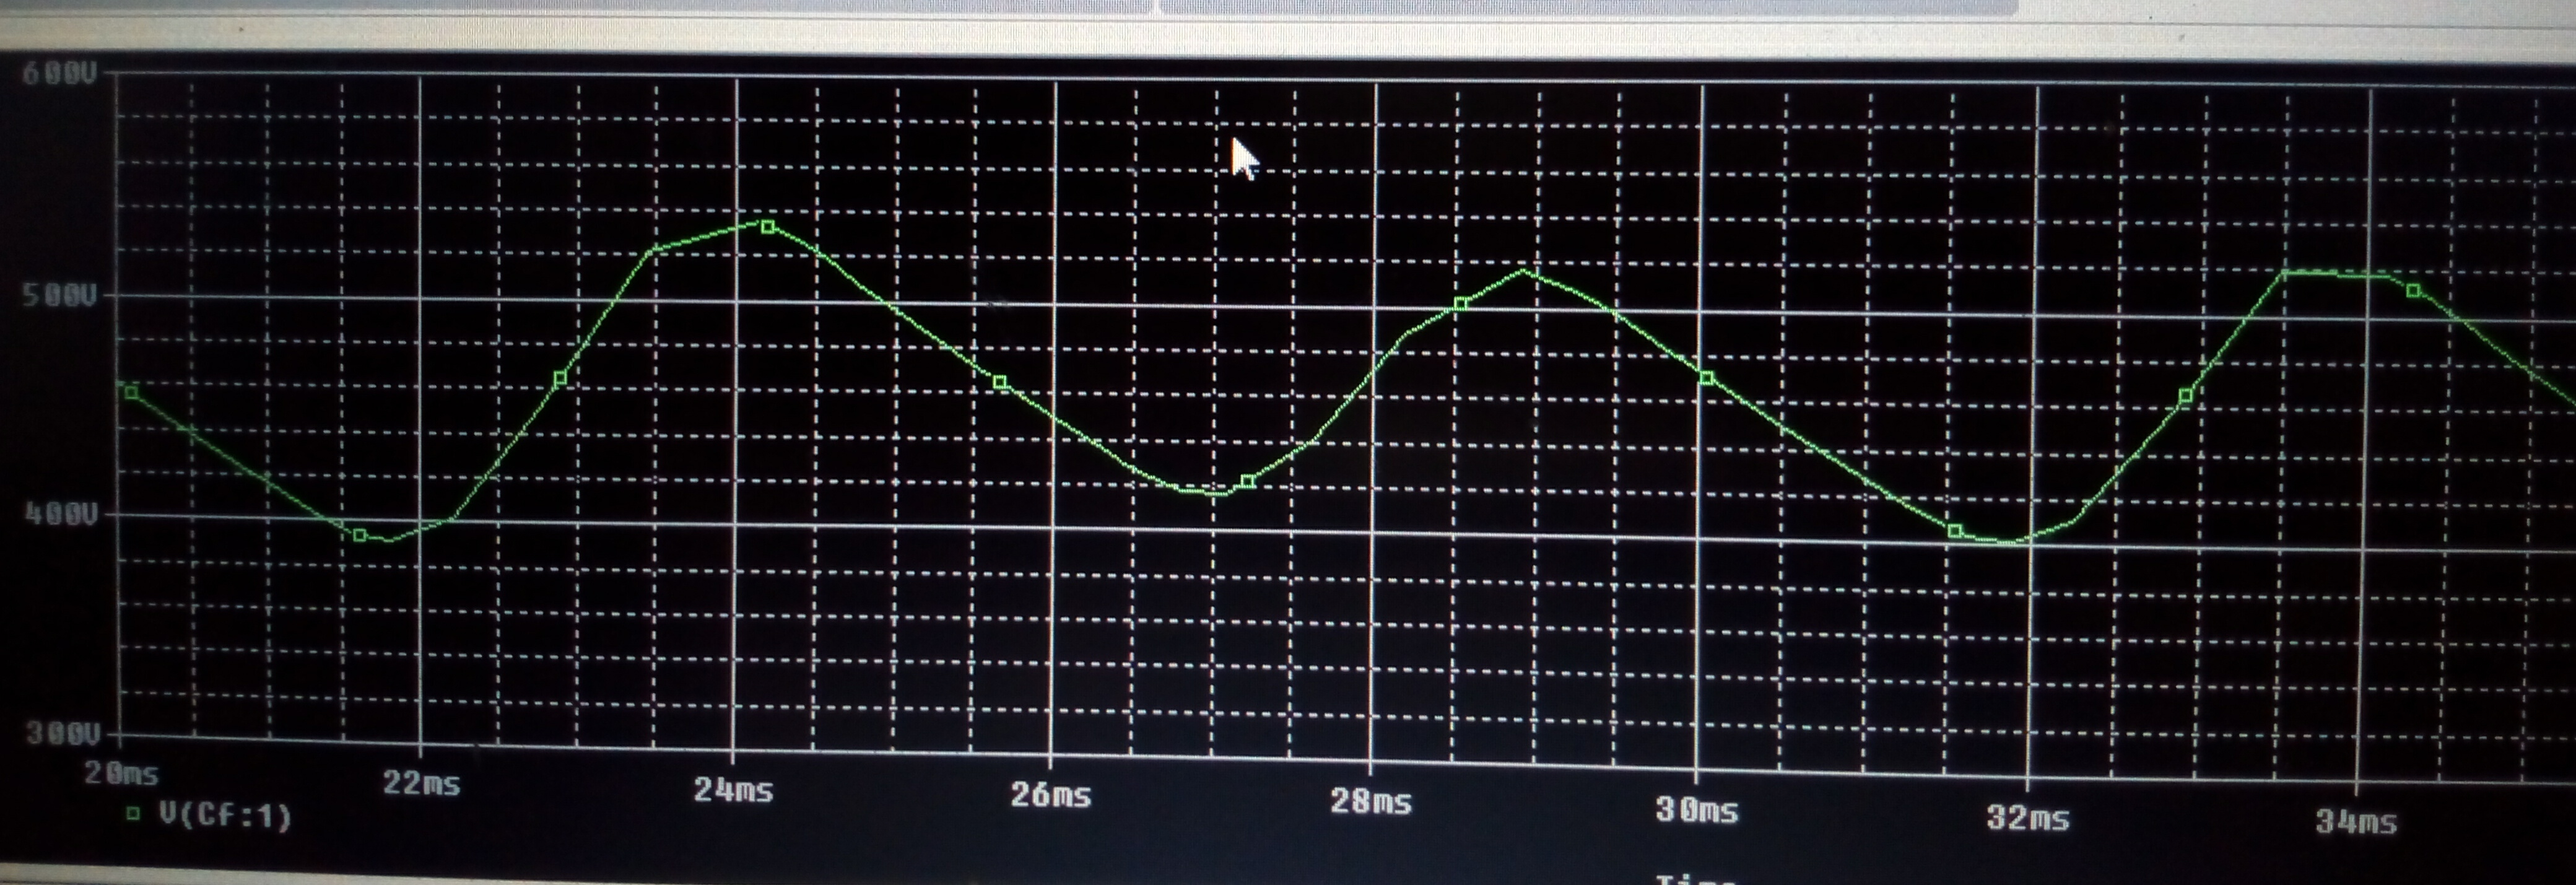
\includegraphics[width=8cm]{Escritorio/Practica 1/19.jpg}
\caption{V(Cf: 0.5mF), Rizado de la tension de salida de la funcion de Cf}
\end{figure}

\begin{figure}[hbtp]
\centering
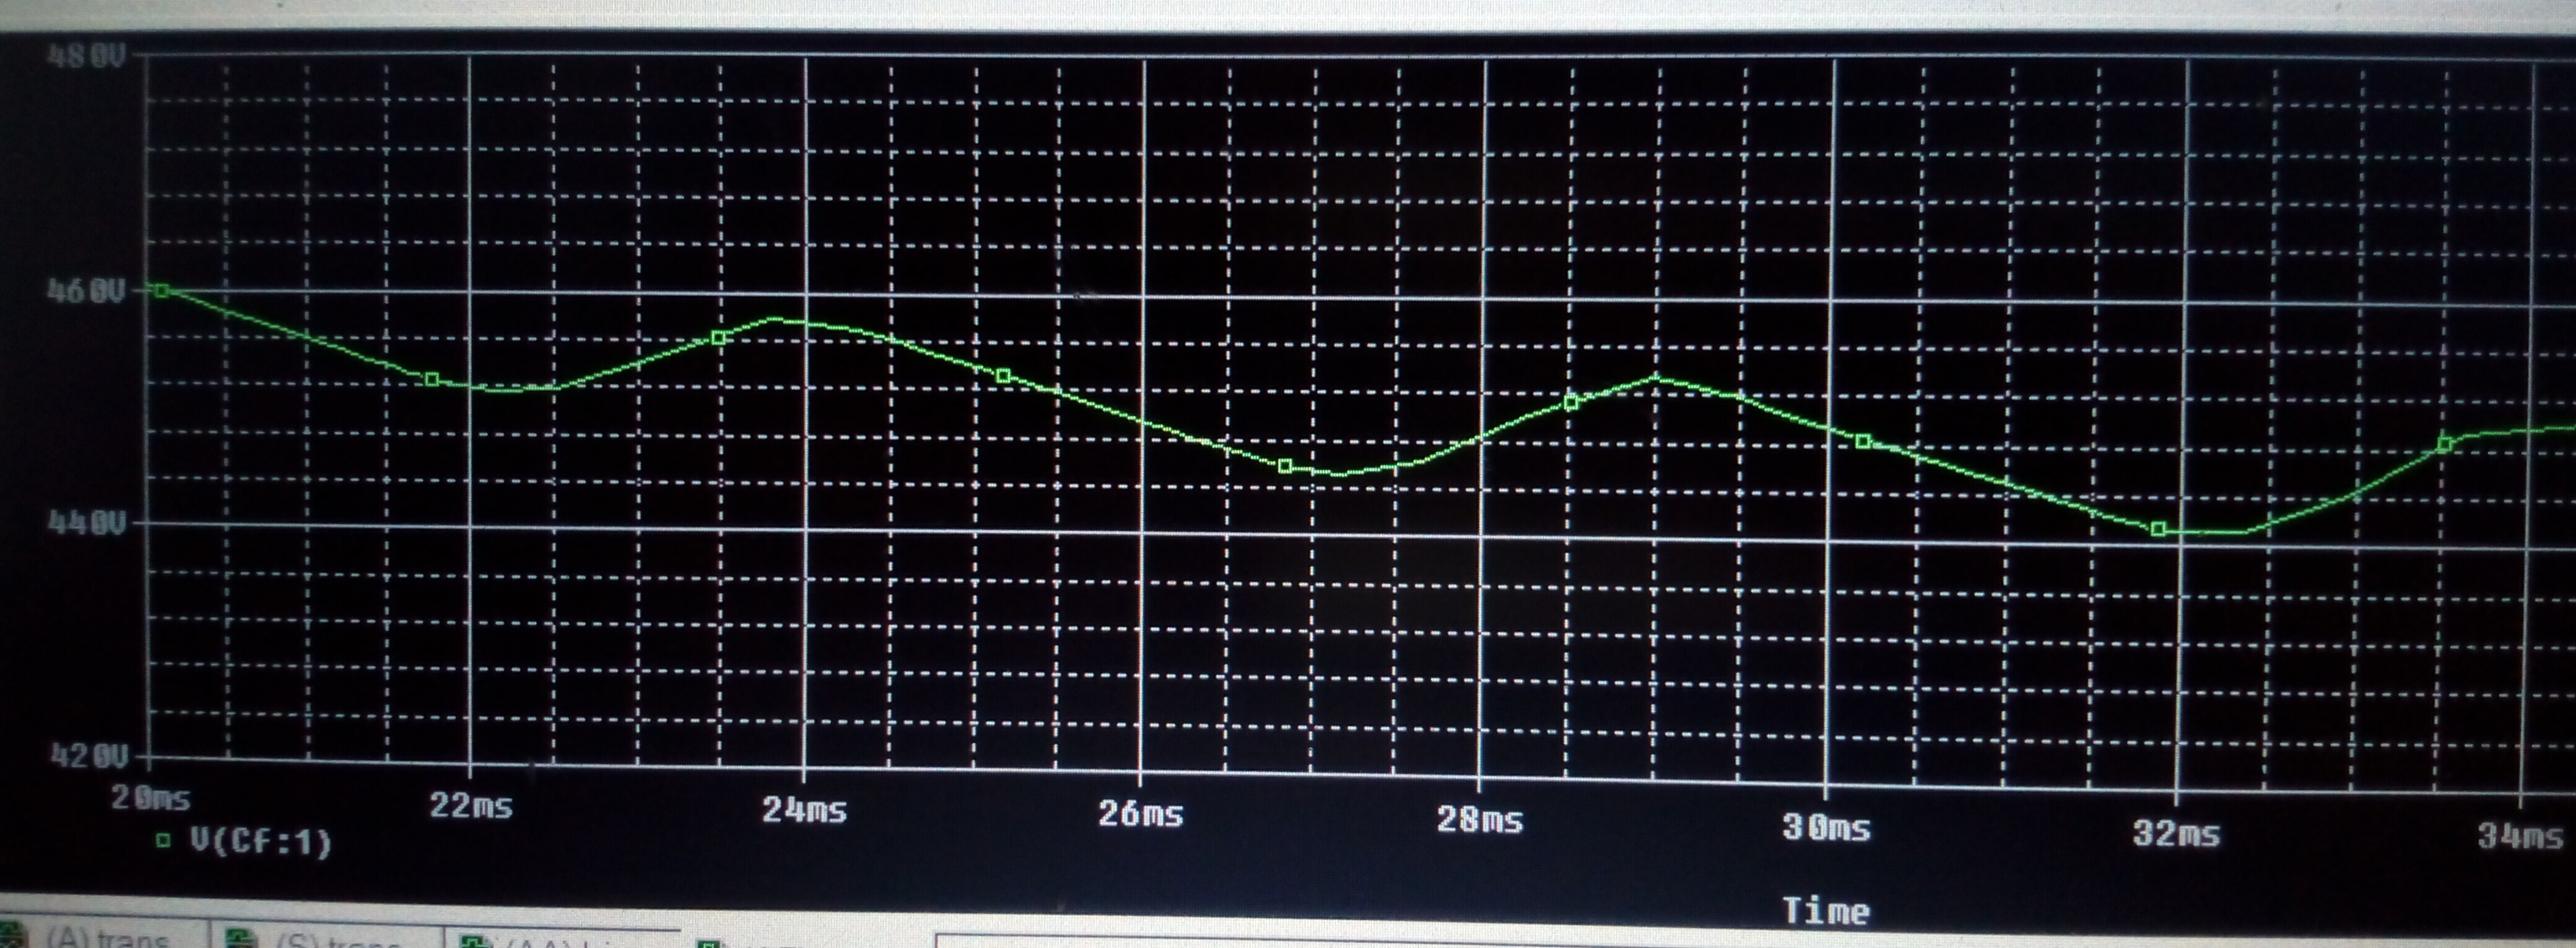
\includegraphics[width=8cm]{Escritorio/Practica 1/20.jpg}
\caption{V(Cf: 5mF), Rizado de la tension de salida de la funcion de Cf}
\end{figure}

\begin{figure}[hbtp]
\centering
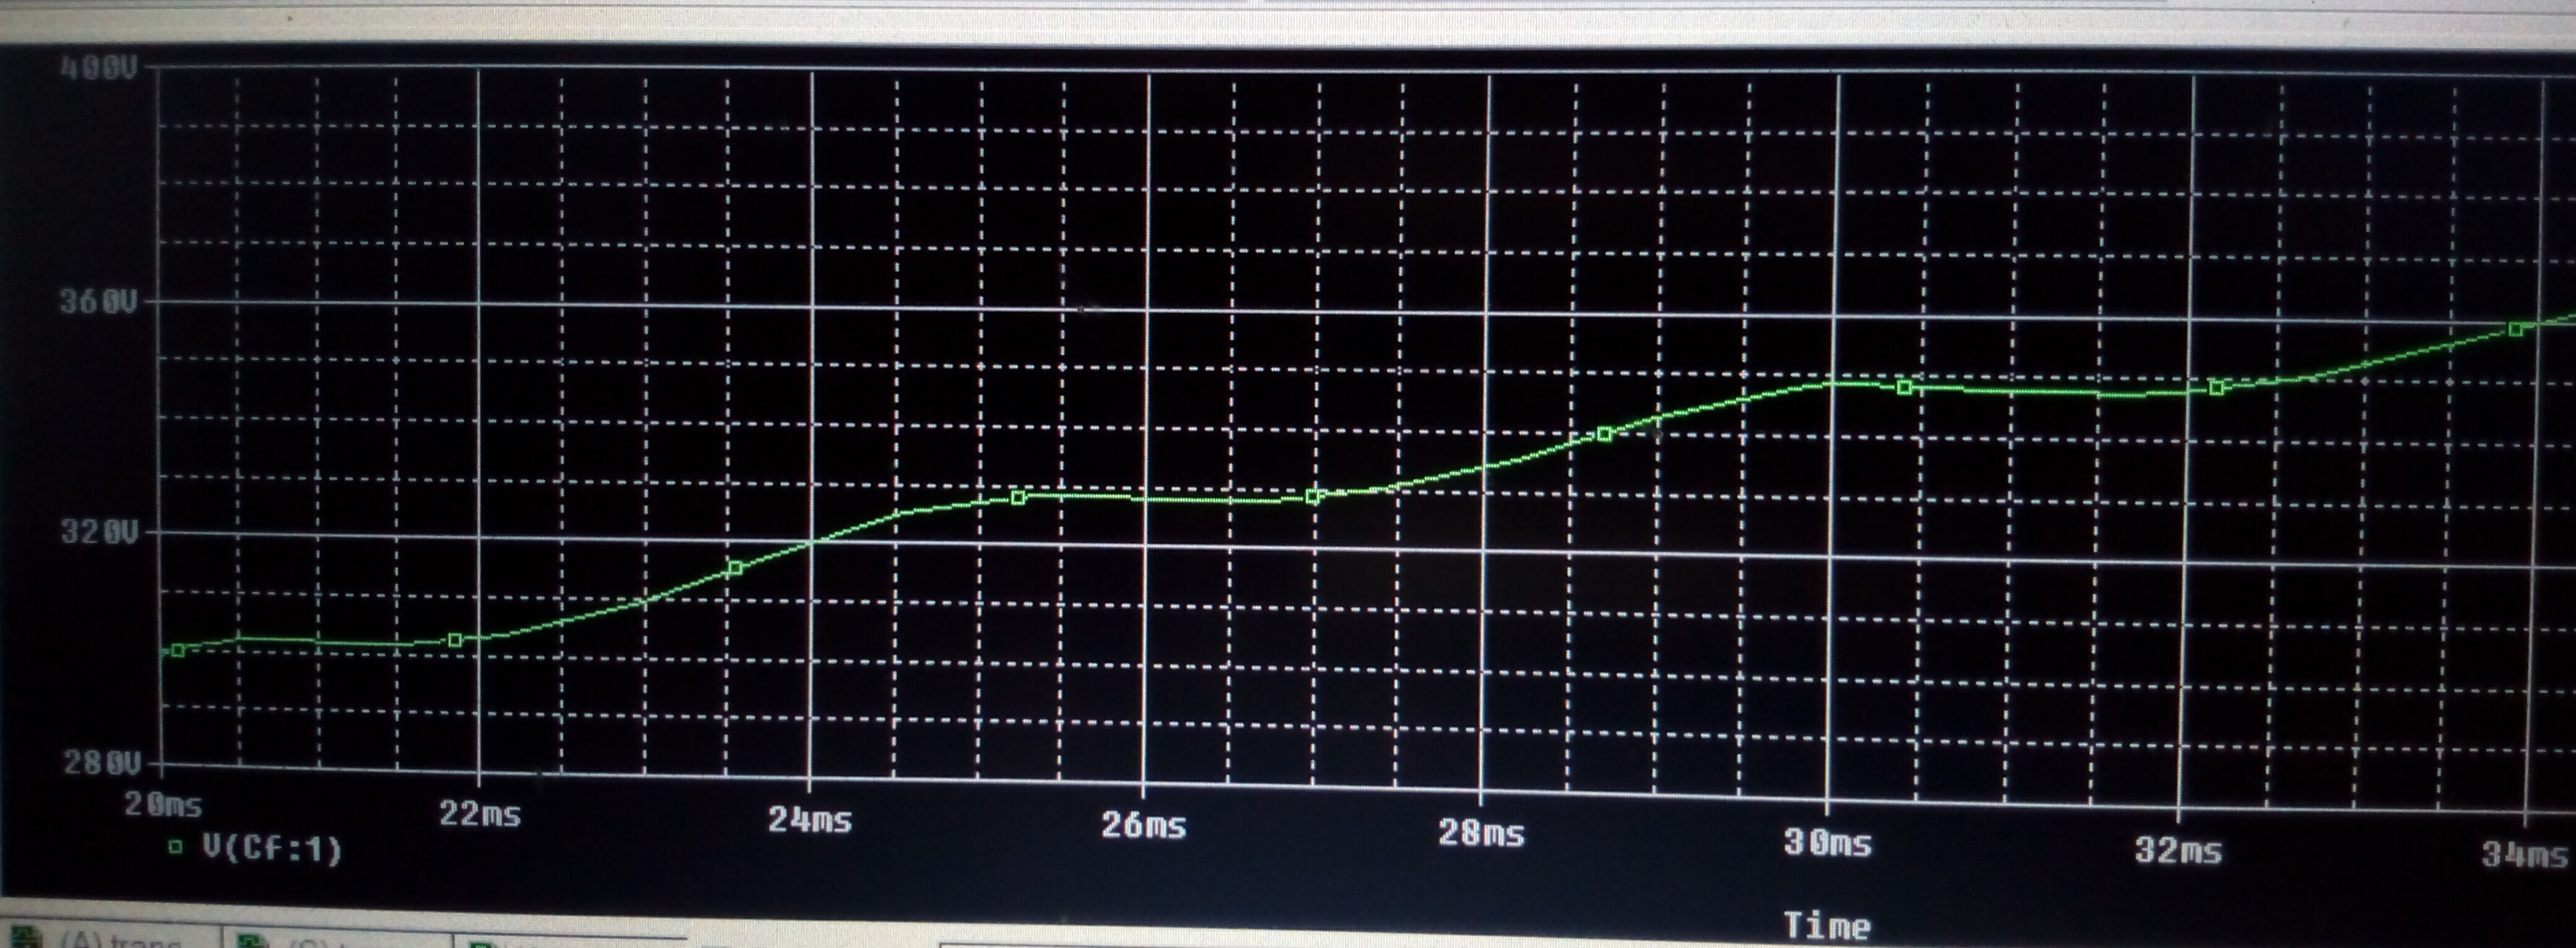
\includegraphics[width=8cm]{Escritorio/Practica 1/21.jpg}
\caption{V(Cf: 20mF), Rizado de la tension de salida de la funcion de Cf}
\end{figure}

\begin{figure}[hbtp]
\centering
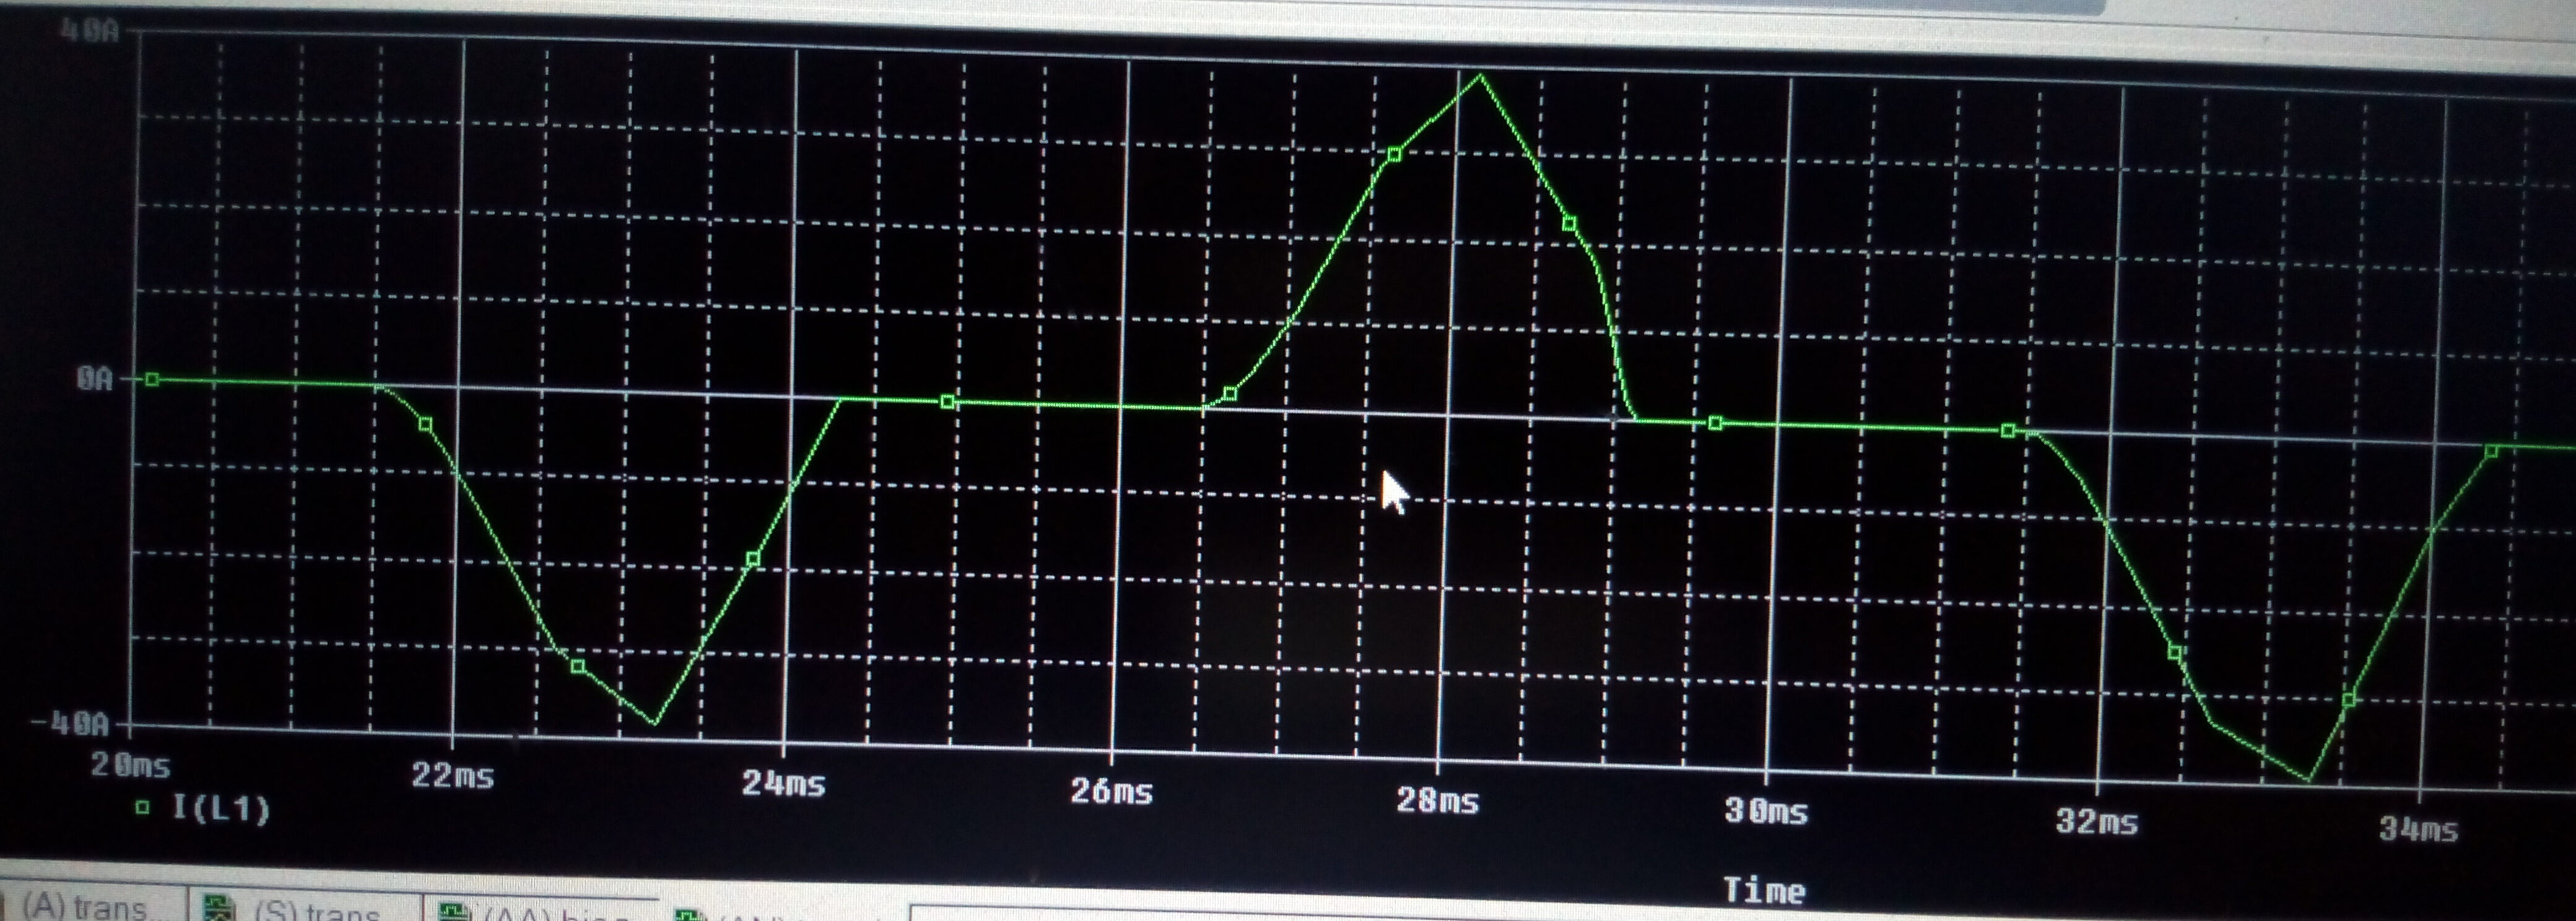
\includegraphics[width=8cm]{Escritorio/Practica 1/22.jpg}
\caption{I(Lr: 0.1mH), corriente del rectificador en funcion Lf}
\end{figure}

\begin{figure}[hbtp]
\centering
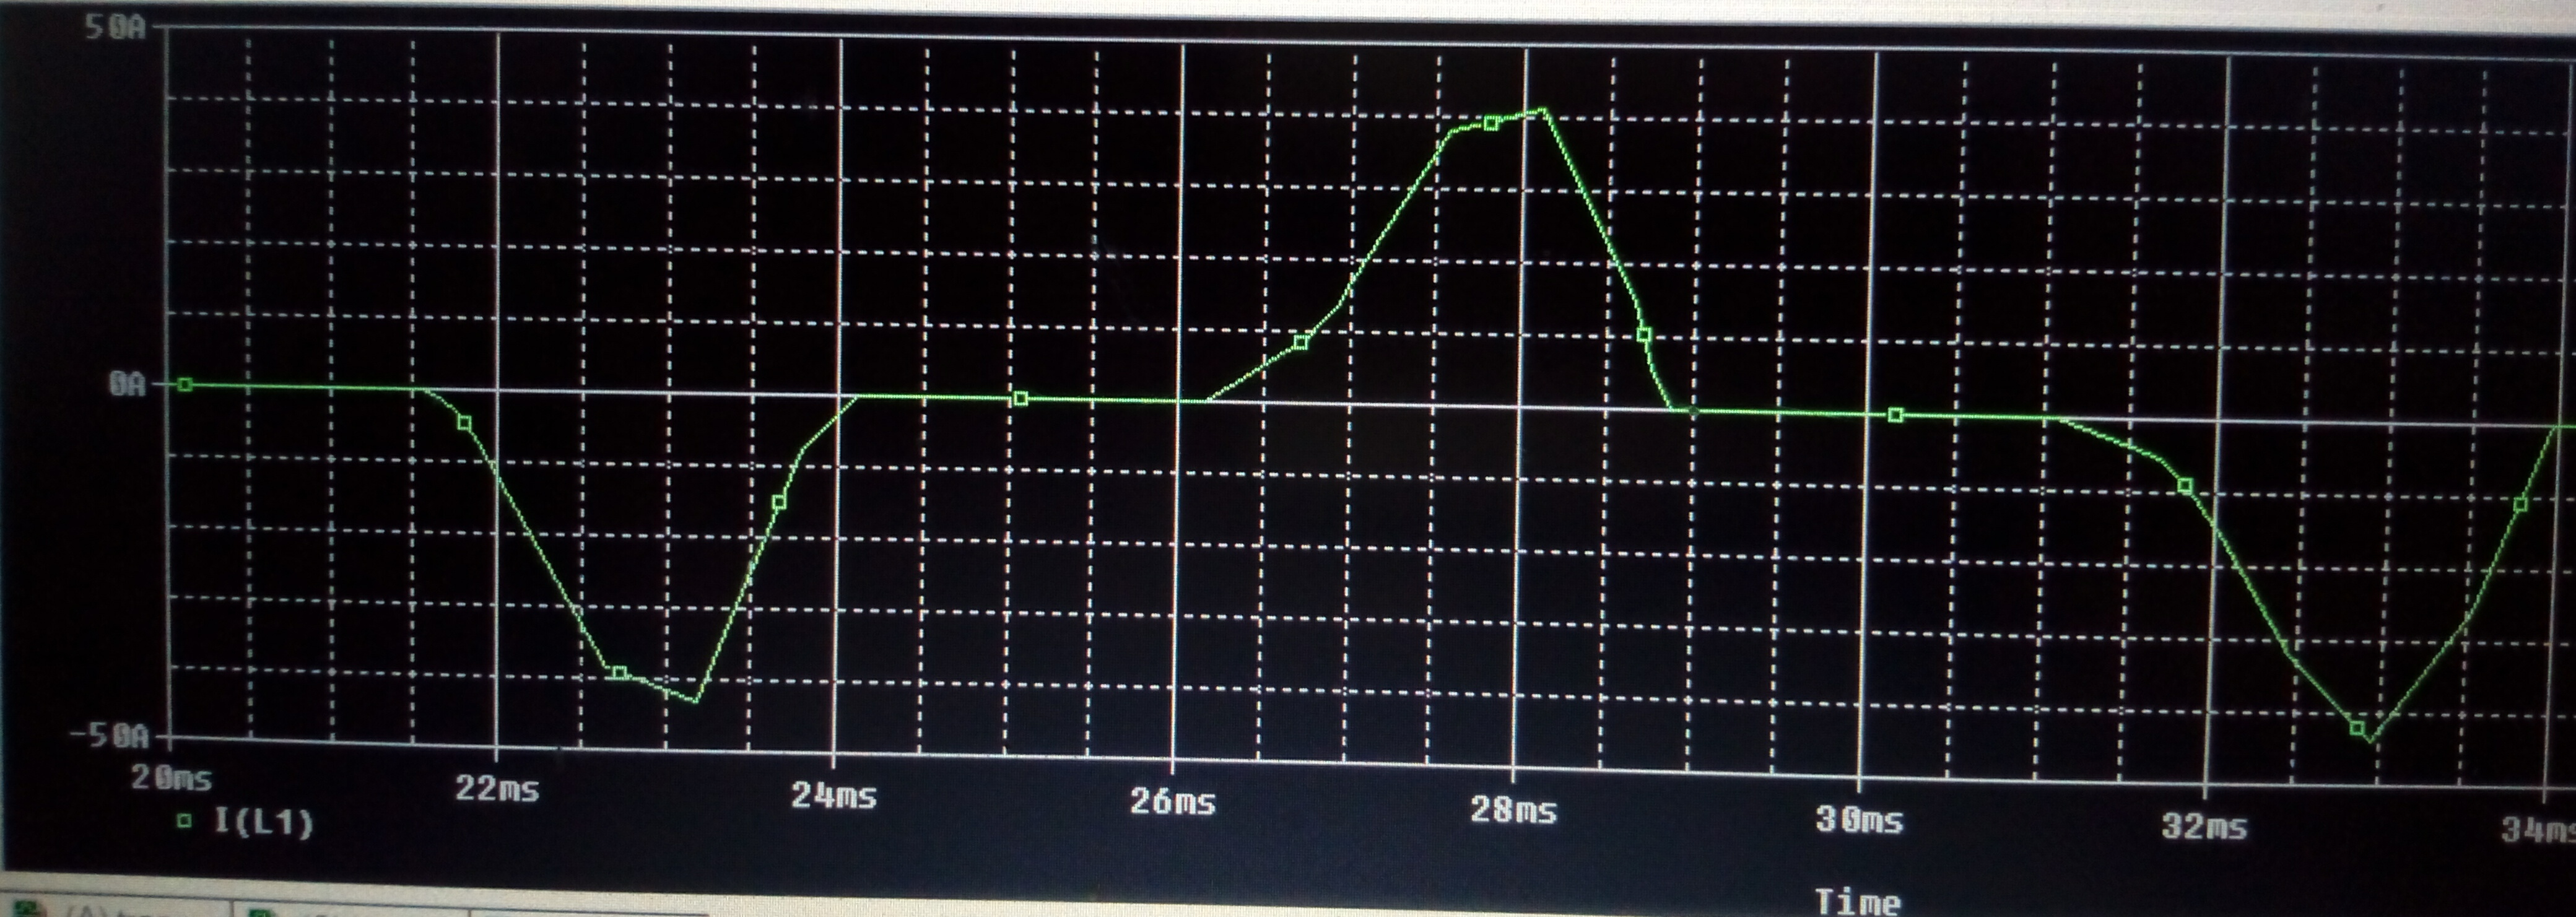
\includegraphics[width=8cm]{Escritorio/Practica 1/24.jpg}
\caption{I(Lr: 0.5mH), corriente del rectificador en funcion Lf}
\end{figure}

\begin{figure}[hbtp]
\centering
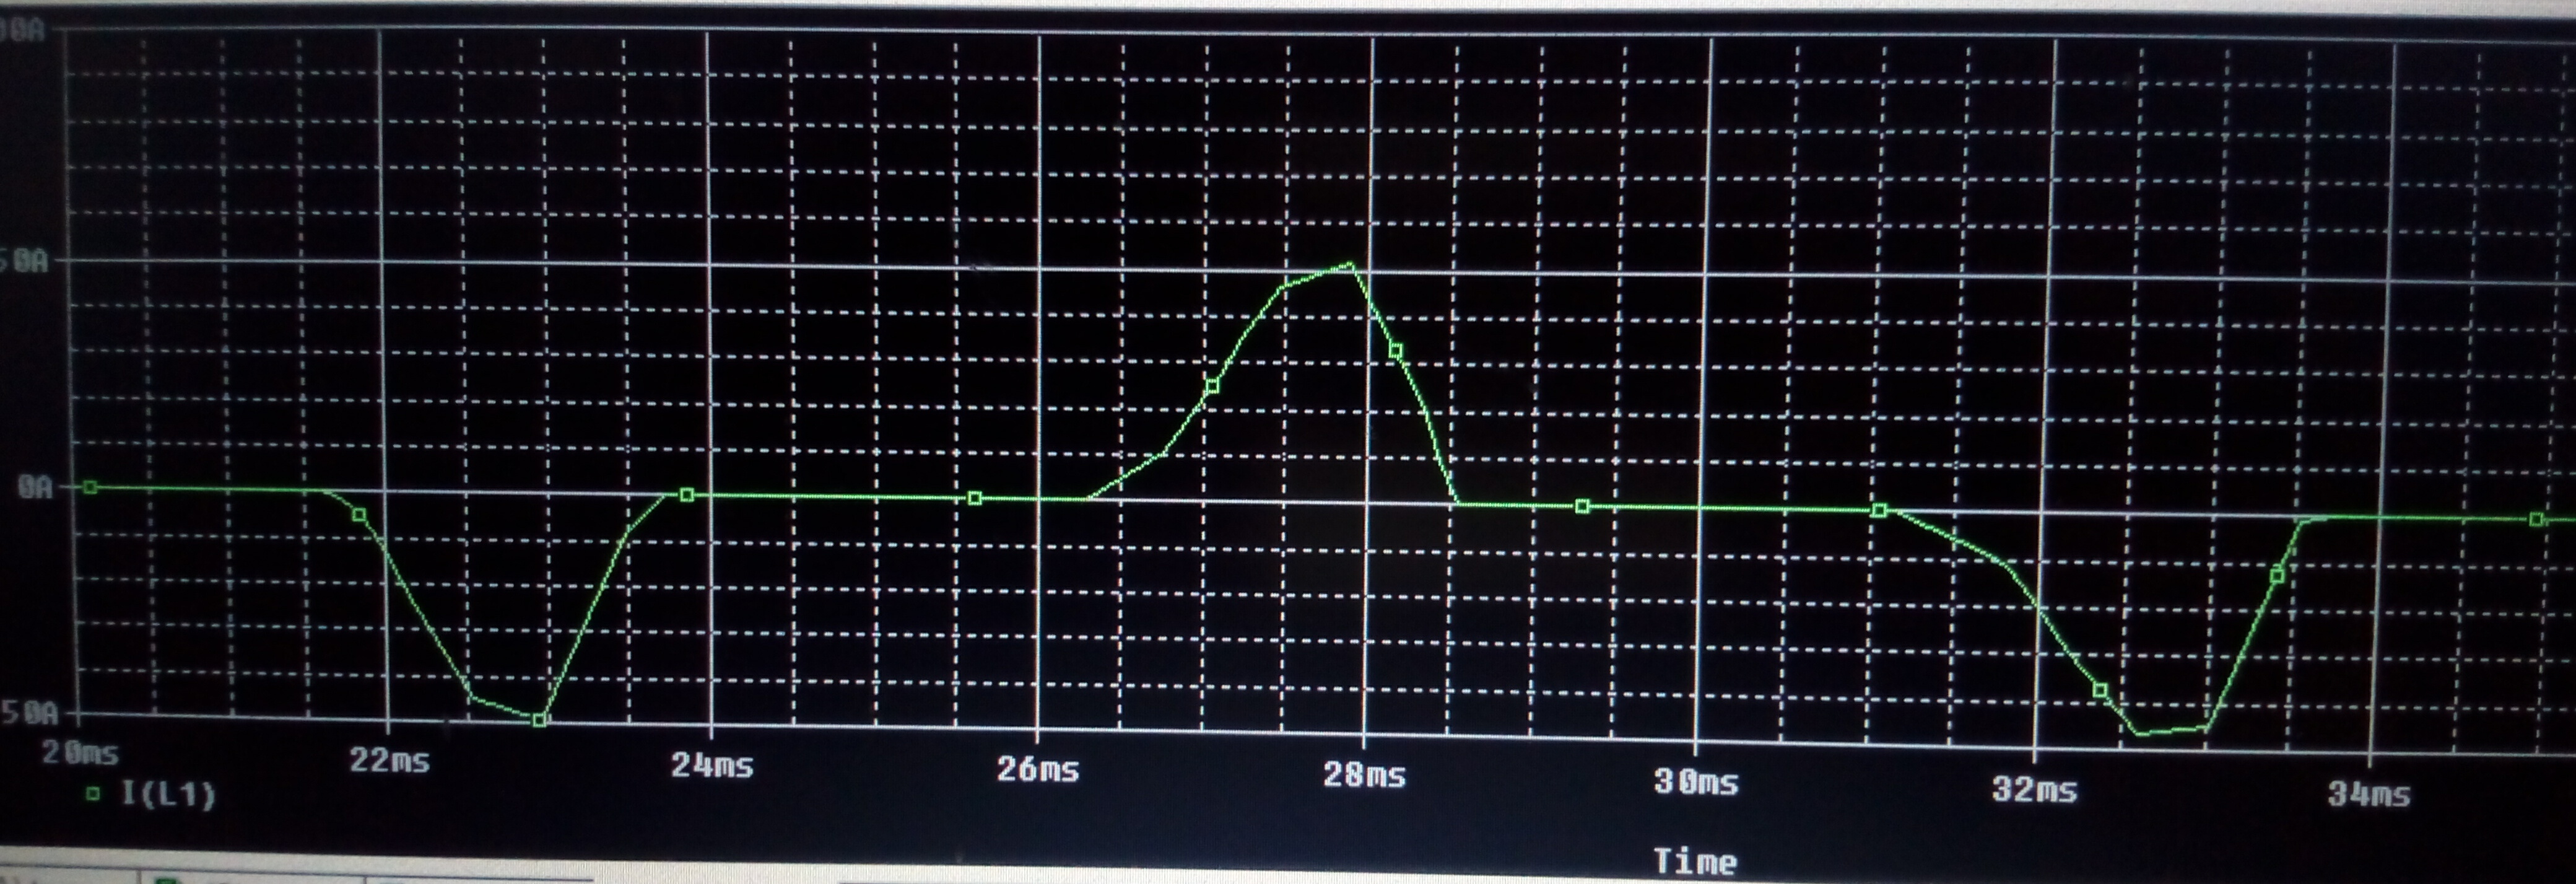
\includegraphics[width=8cm]{Escritorio/Practica 1/25.jpg}
\caption{I(Lr: 1mH), corriente del rectificador en funcion Lf}
\end{figure}

\begin{figure}[hbtp]
\centering
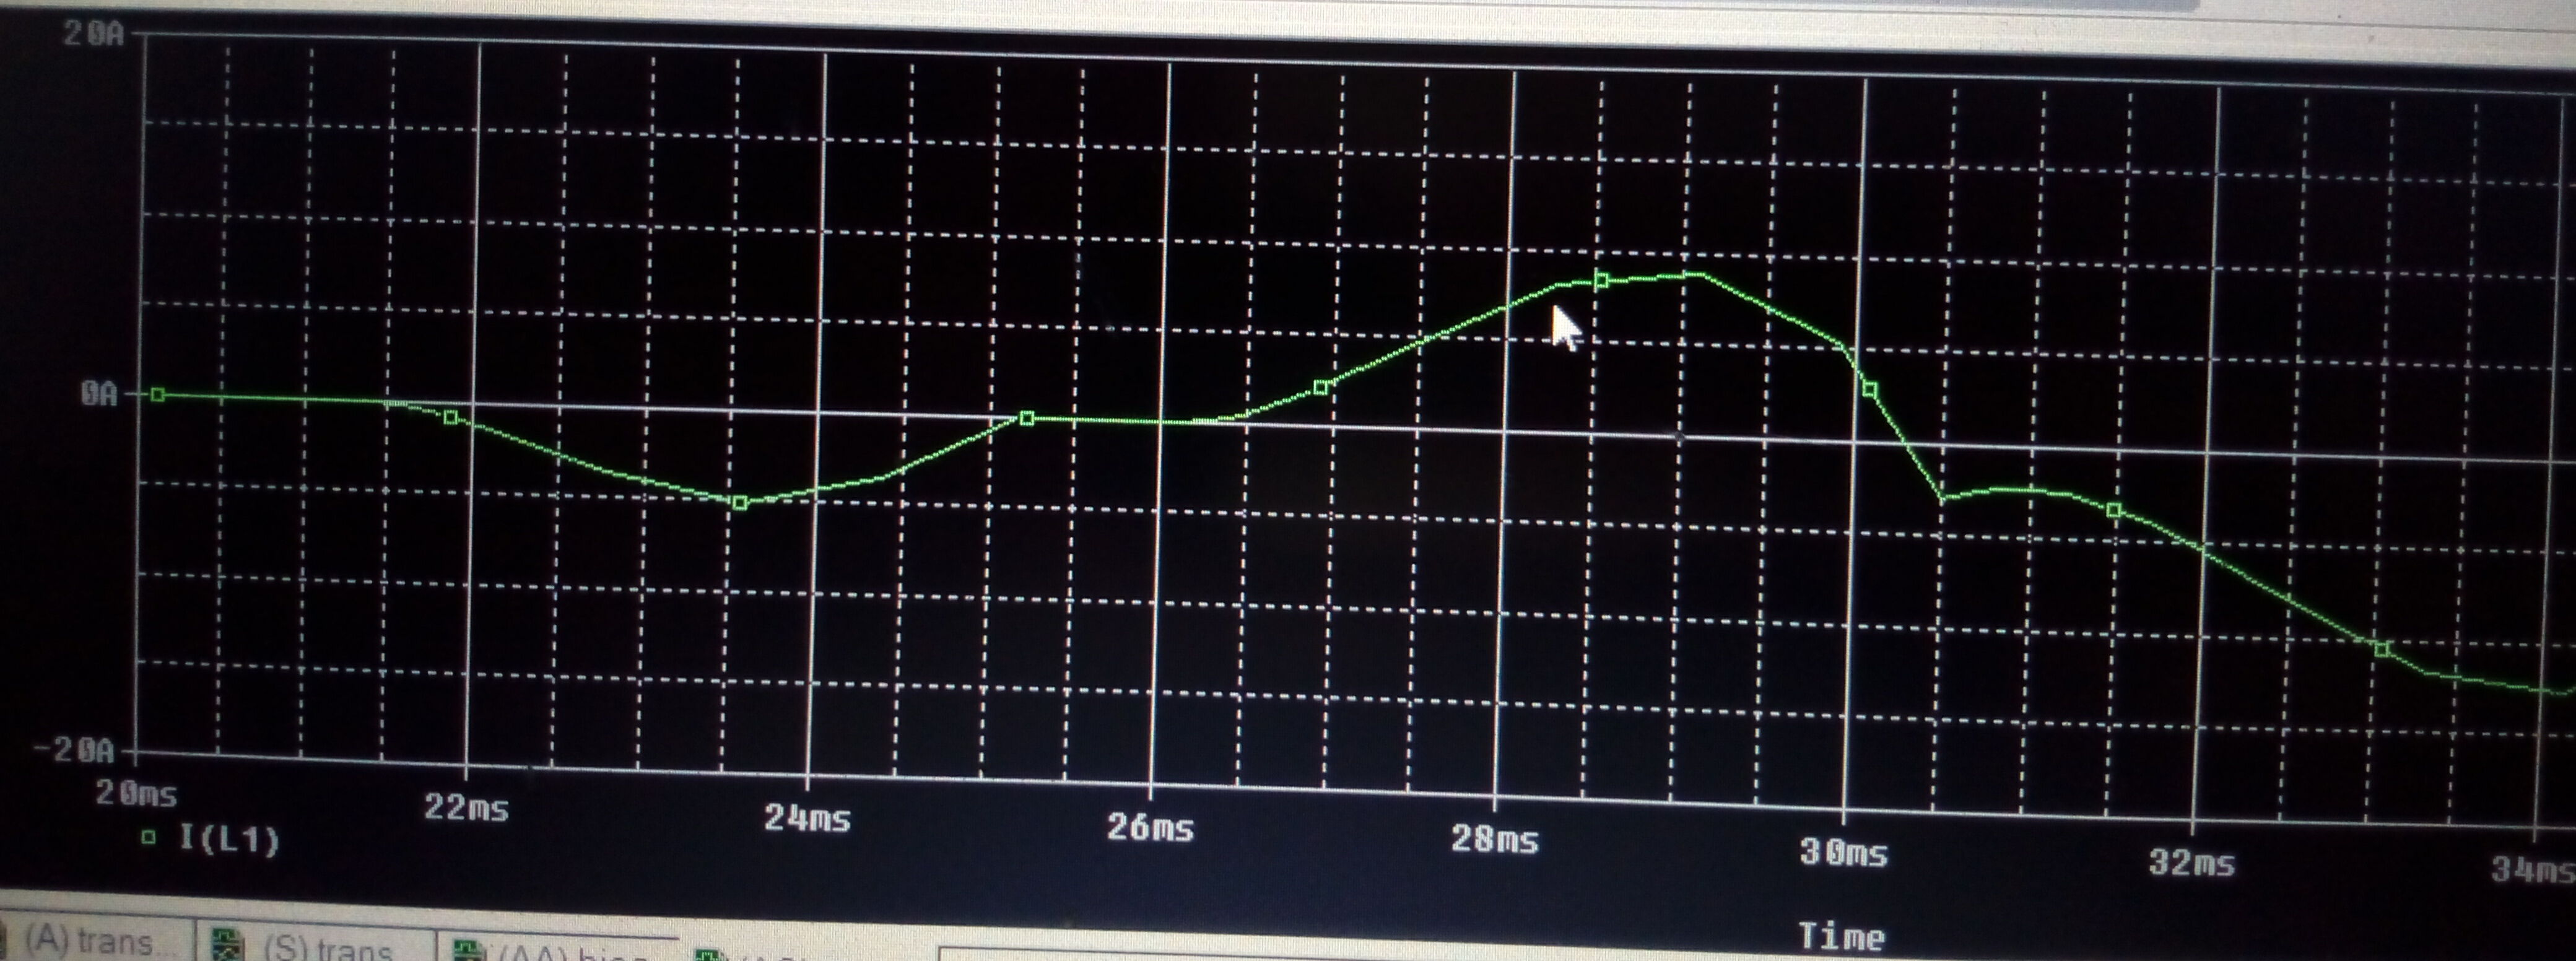
\includegraphics[width=8cm]{Escritorio/Practica 1/23.jpg}
\caption{I(Lr: 20mH)corriente del rectificador en funcion Lf}
\end{figure}


\begin{figure}[hbtp]
\centering
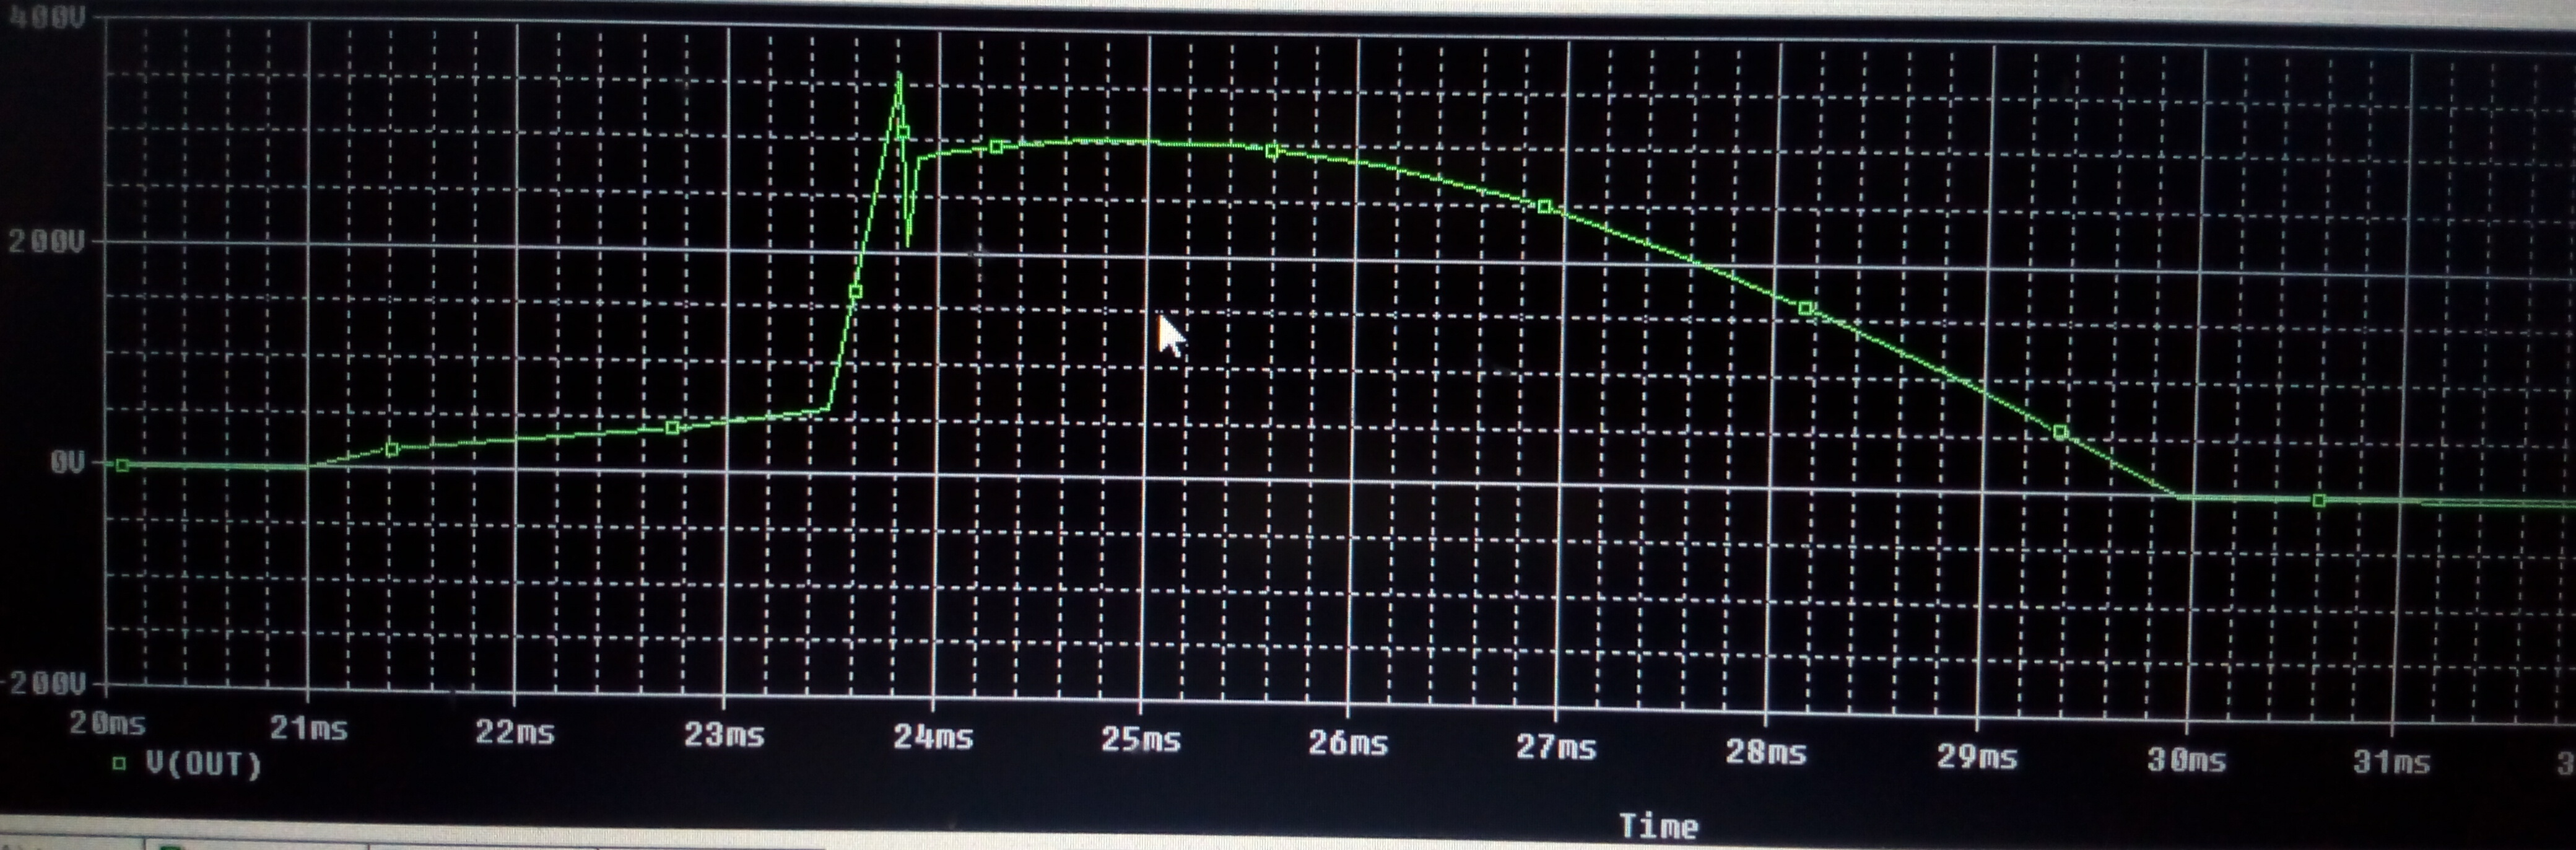
\includegraphics[width=8cm]{Escritorio/Practica 1/26.jpg}
\caption{V(out), Perdida de tension debido a la conmutacion de diodos}
\end{figure}

\begin{figure}[hbtp]
\centering
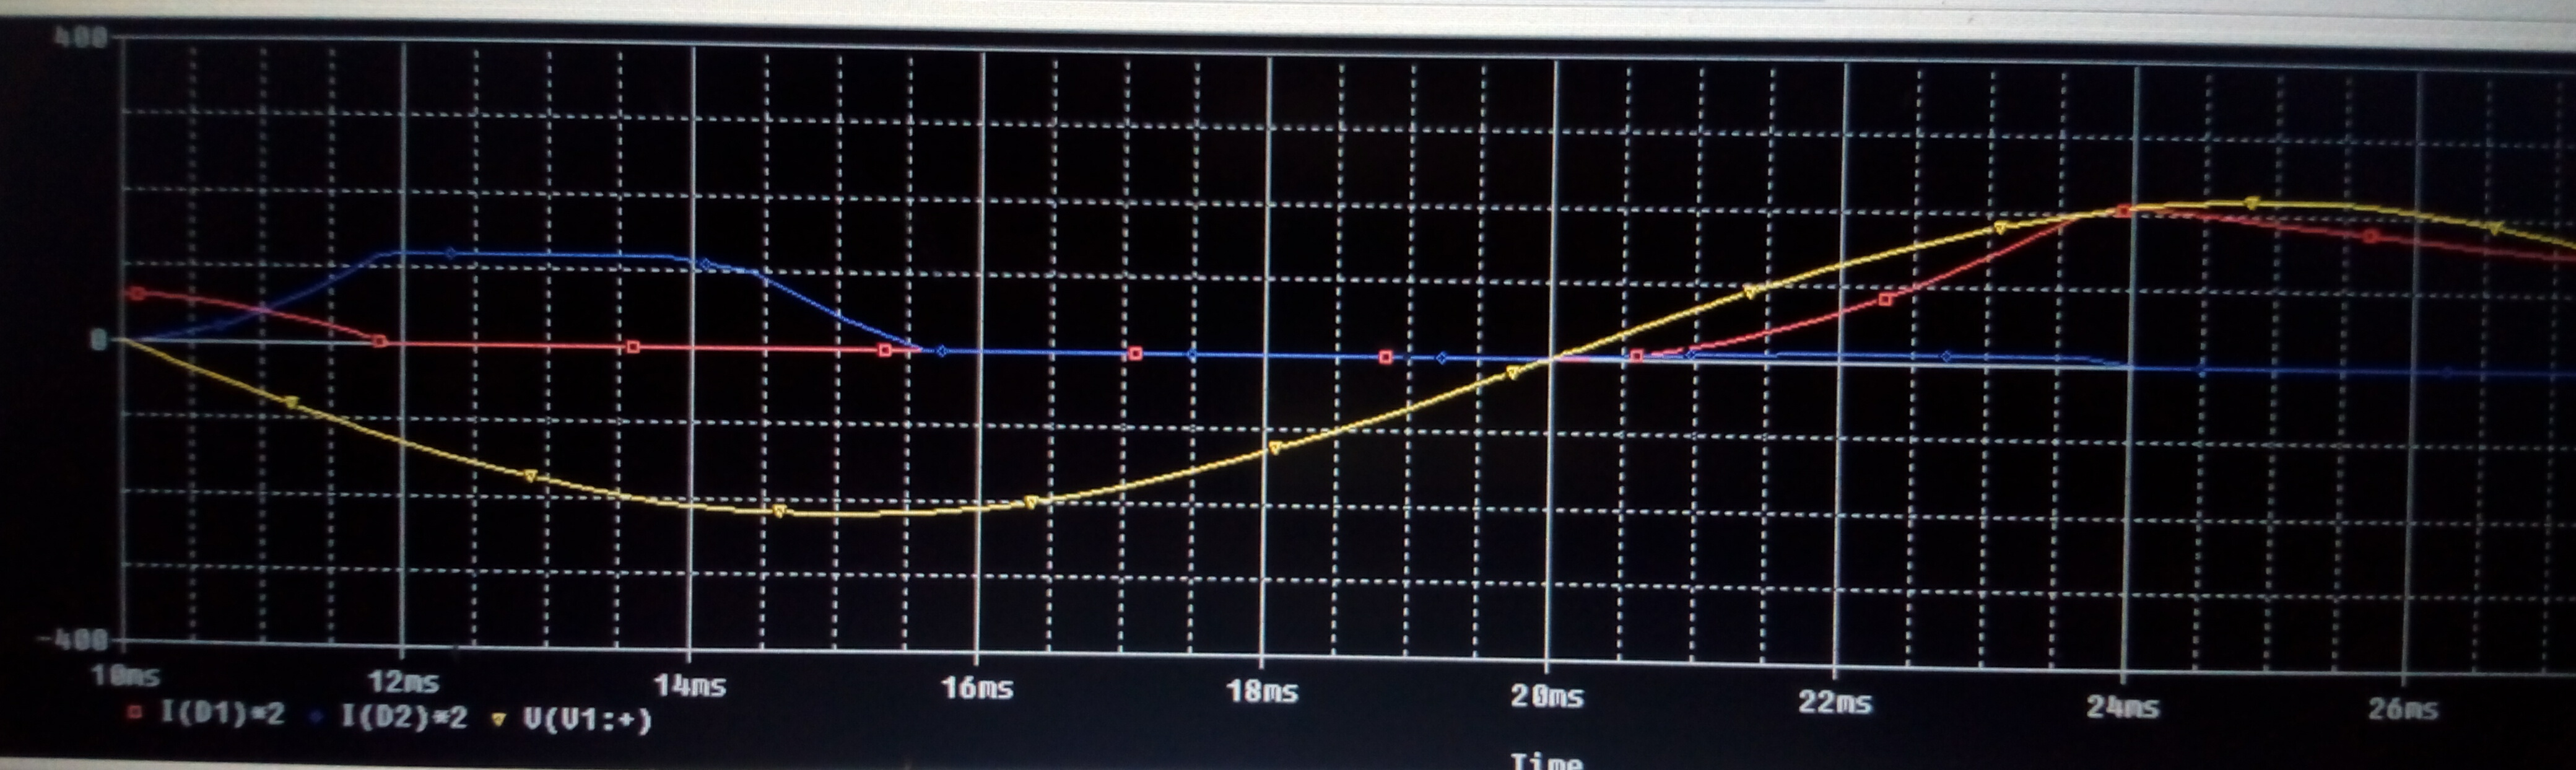
\includegraphics[width=8cm]{Escritorio/Practica 1/27.jpg}
\caption{I(D1), I(D2), V(V1), Perdida de la tension debido a la conmutacion de diodos}
\end{figure}

\begin{figure}[hbtp]
\centering
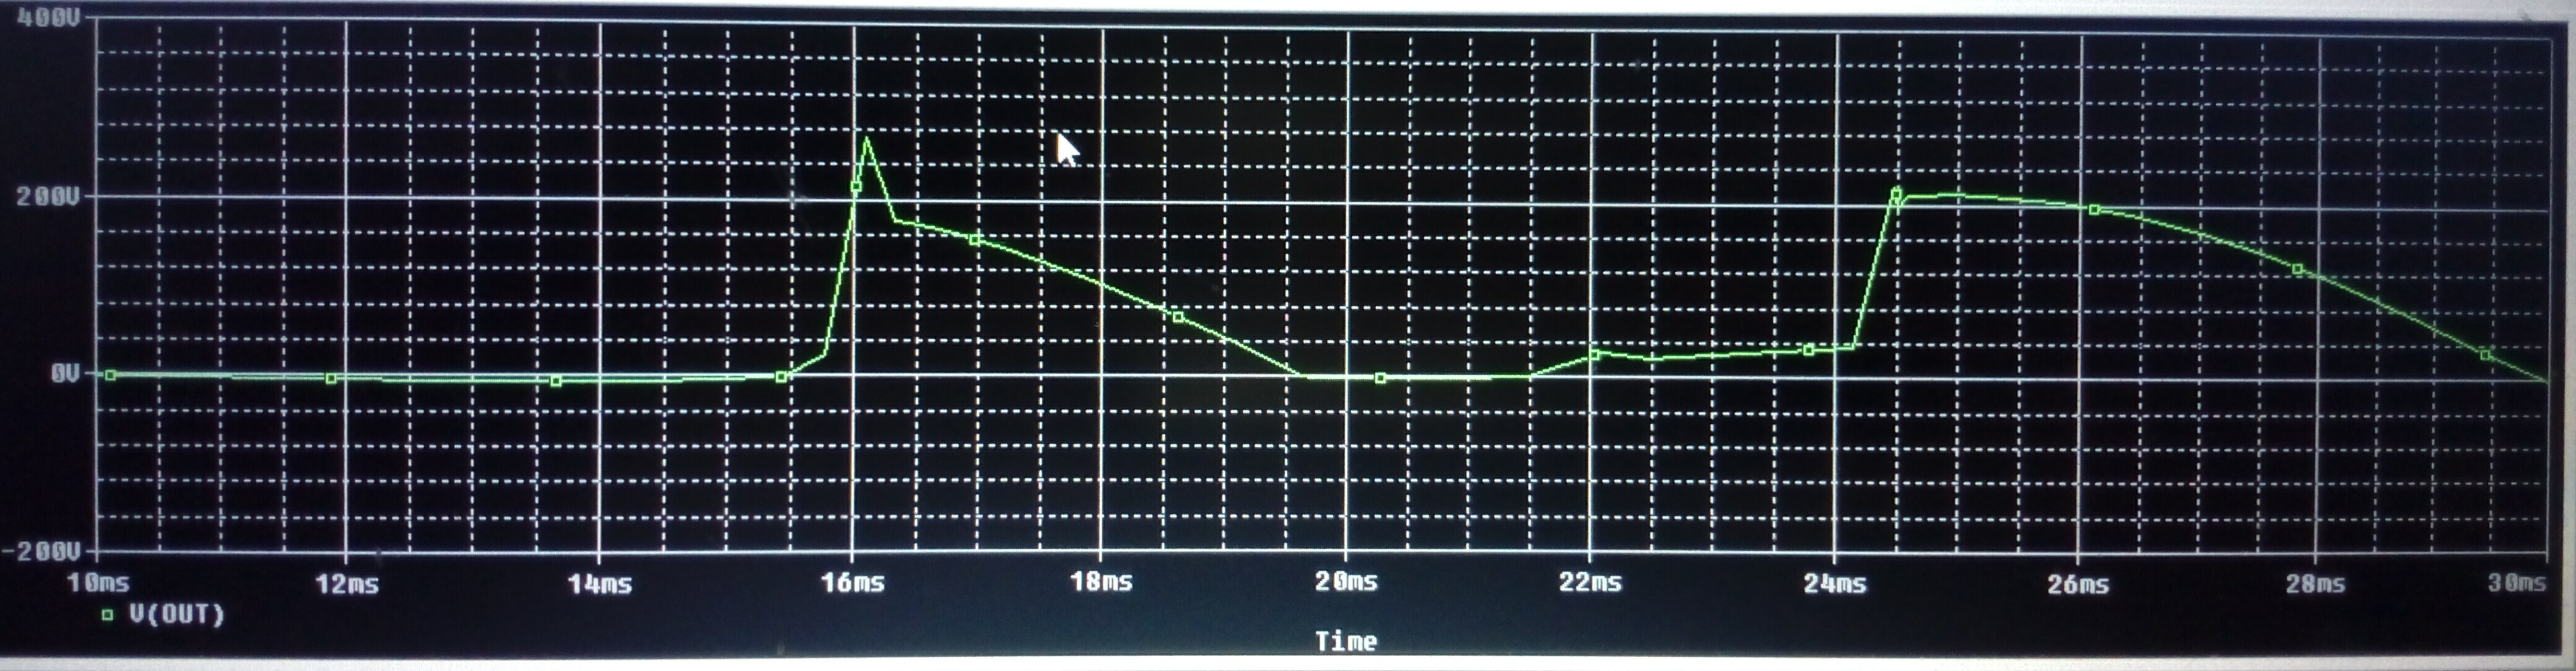
\includegraphics[width=8cm]{Escritorio/Practica 1/28.jpg}
\caption{V(out), efectos de la conmutacion entre diodos en la salida del rectificador monofasico}
\end{figure}

\begin{figure}[hbtp]
\centering
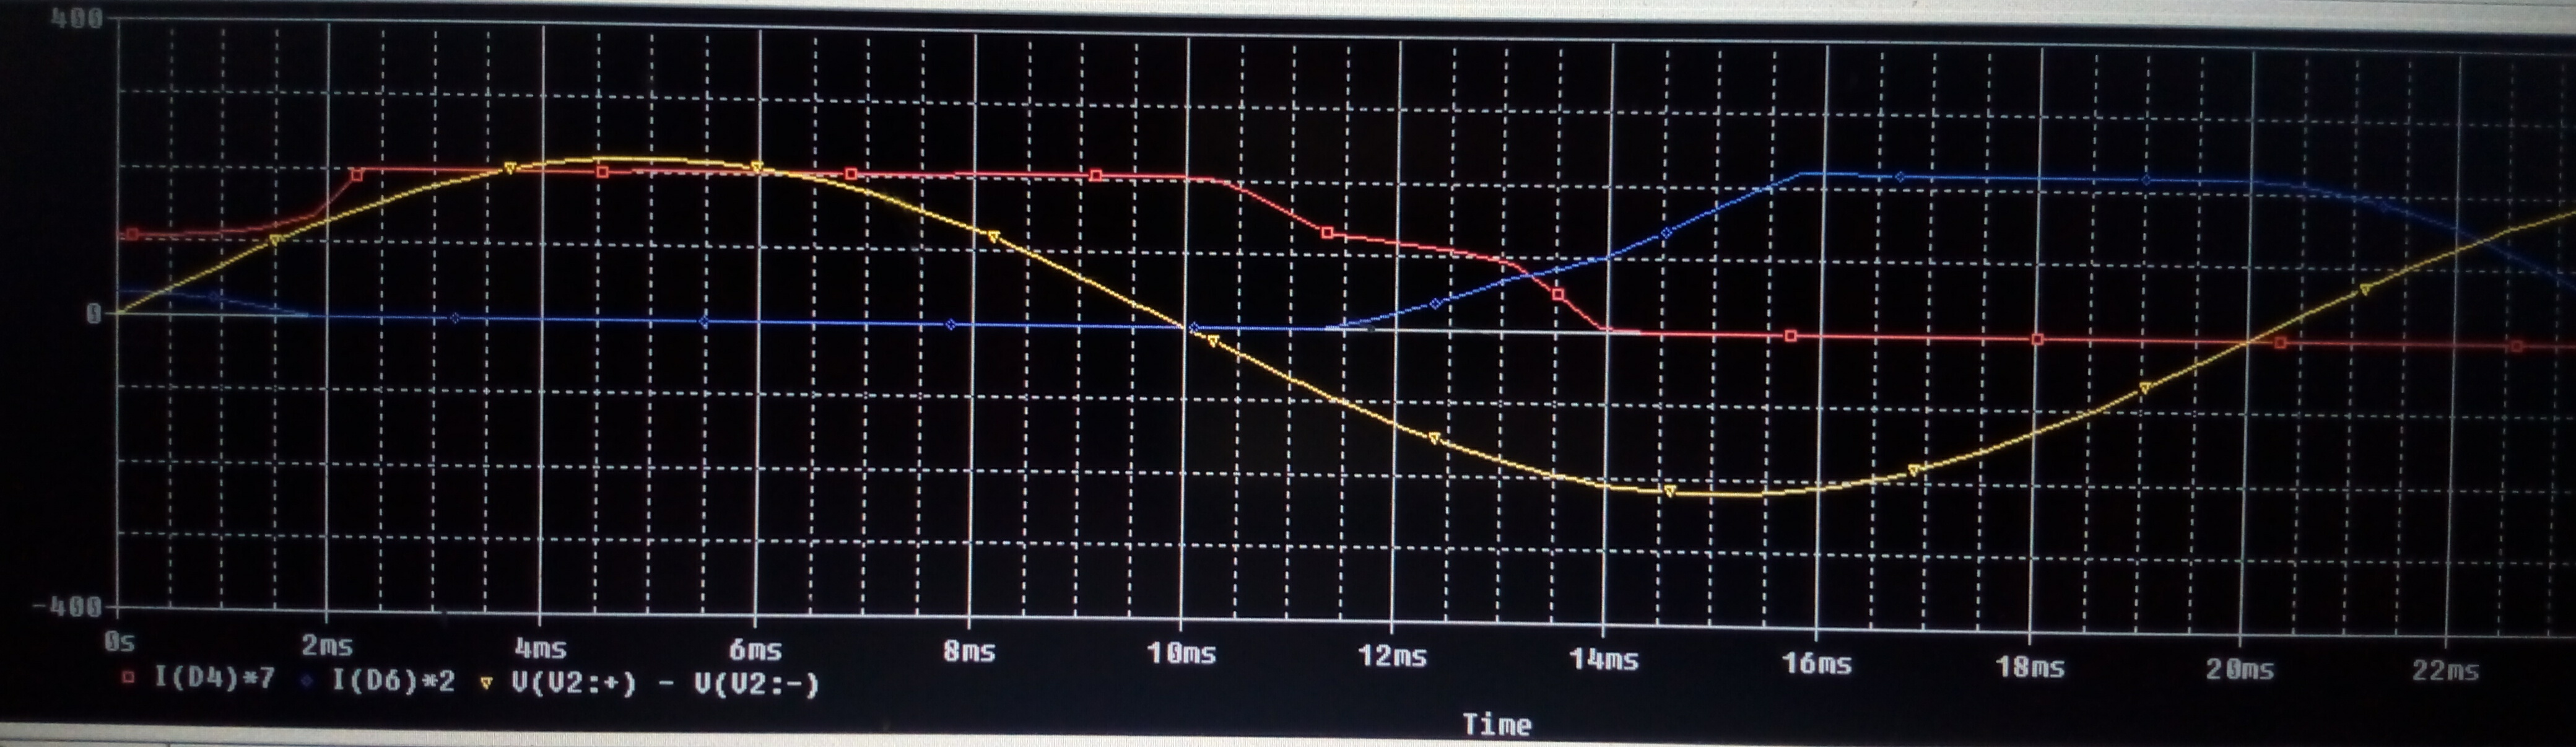
\includegraphics[width=8cm]{Escritorio/Practica 1/29.jpg}
\caption{I(D3)*20, I(D4)*20, V(V1), Efectos de la conmutacion entre diodos en la salida del rectificador monofasico}
\end{figure}

\begin{figure}[hbtp]
\centering
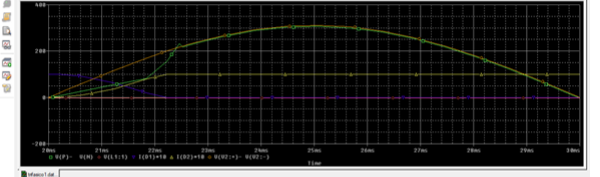
\includegraphics[width=8cm]{Escritorio/Practica 1/30.png}
\caption{V(P)-V(n), I(D3)*2, (V1:+)-V(V1:-), Perdida de tensio en el rectificador trifasico debido a las conmutaciones entre diodos}
\end{figure}

\section{Conclusion:}
\subsubsection{Conclusion:Guzman Jaime.}
En esta practica aprendimos a utilizar el software de ORCAD para realizar
las simulaciones correspondientes en los diferentes circuitos, esto de mi parte
fue algo nuevo ya que nunca habia utilizado este software de diseo sin em-
bargo cumplio las espectativas que se tenian de el, los esquematicos cada uno
cumple una funcion especifica o contiene un tipo de diferente de caracteristica
que lo diferencia de los demas, algunos tenian tres fuente de corriente otros
tenian un puente de diodos adjuntado a una bobina o capacitores y cada
configuracion realiza alguna funcion , algus amplifican la seal de entrada en
la salida y algunos otros retrasan la seal formando un pico desfasado o una
onda desfasada, algunos otros rectifican la onda completa generando de una
corriente alterna a una practicamente directa o incluso algunos otros rectifi-
can solamente la mitad de la onda estos diferentes aspectos de cada circuito,
el realizarlos en pcb al igual que en esquematico y cada una de sus ondas
fue muy interesante ademas de ayudar mucho a la formacion de los alumnos
en cuanto a la electronica de potencia ademas de el software de diseo de
circuitos.\\

\subsection{Conclusion: Francisco Rodriguez}
Los diodos juegan un papel muy importante a la hora de trabajar, con fuentes de potencia alta, ya que estos nos dejan controlar, y seguir a pasos de manera eficiente y correcta lo que hacemos directramente con el voltaje, que consumimos nosotros dia con dia, dejando en margen el error que cometemos en ocasiones, al no medir o no saber utilizar de manera eficiente, nuestro sistema o circuito.\\
En todo caso la buena estructura con los argumentos dados en estos terminos, en practica pueden llegar a ser muy utiles, tanto estos componentes, como la aplicacion y utilidad que tienen, dejando asi una buena enseñanza, para el estudiante, y para el empresario, o cientifico a futuro.

\end{document}